\documentclass[12pt, dvipsnames]{article}

\usepackage[utf8]{inputenc}
\usepackage{xcolor}
\usepackage[a4paper, left=3cm, right=3cm, top=4cm]{geometry}
\usepackage{graphicx}
\usepackage[sorting=none]{biblatex}
\usepackage[english,german]{babel} 
\usepackage{minted}
\usepackage{csquotes}
\usepackage{svg}
\usepackage{amsmath}
\usepackage{datetime}
\usepackage{hyperref}
\usepackage[font={small,it}]{caption}
\usepackage{acronym}
\usepackage{listings}
\usepackage[T1]{fontenc}
\usepackage{subfig}

\usepackage{CJKutf8}

\usepackage{amssymb}
\usepackage{pifont}
\usepackage{wasysym}

\usepackage{tikz}
\usepackage{tkz-euclide}
\usetikzlibrary{automata, positioning, arrows}

\usepackage{pgfplots}

% example texts
\usepackage{blindtext}
\usepackage{lipsum}

% Table
\usepackage{tabularx}
\usepackage{longtable}





\selectlanguage{german}
%\selectlanguage{english}

%%%%%%%%% Line Thickness %%%%%%%%% 
\newcommand{\HRule}{\rule{\linewidth}{0.5mm}}

\addbibresource{bib/books.bib}

\pagenumbering{gobble}

\begin{document}
\begin{titlepage}
\centering
%%%%%%%%% Heading %%%%%%%%%
\title{Bachelorarbeit}
\vspace{2cm}
\vspace{1cm}
\textsc{\LARGE \\ Universität Kassel}\\[0.5cm] % Major heading
\textsc{\large Bachelorarbeit im Fachgebiet}\\[0.5cm] % Small heading
\textsc{\large Gender/Diversity in Informatiksystemen}\\[0.5cm] % Small heading

%%%%%%%%% Title %%%%%%%%%
\vspace{1.4cm}
\line(1,0){200}
\vspace{0.4cm}
{ \huge \bfseries \\ Konzeption und Entwicklung eines Rollenspiels}\\[0.2cm]
\line(1,0){200}
\vspace{1.5cm}\\

%%%%%%%%% Author %%%%%%%%%
\vspace{5cm}
\begin{minipage}{0.4\textwidth}
\begin{flushleft}
\large\emph{Author:}\\
Julian Holfeld\\
\end{flushleft}
\end{minipage}~
\begin{minipage}{0.4\textwidth}
\begin{flushright}
\large\emph{Erstprüfer:}\\
Prof. Dr. phil. Claude Draude\\
\large\emph{Zweitprüfer:}\\
Prof. Dr. rer. nat. Albert Zündorf
\end{flushright}
\end{minipage}\\[2cm]

%%%%%%%%% Date %%%%%%%%%
{\large \today}\\[2cm]

\vfill % Fill the rest of the page with whitespace
\end{titlepage}

\section*{Eidesstattliche Erklärung}

Hiermit erkläre ich, dass ich die vorliegende Arbeit selbstständig und nur mit den nach der Prüfungsordnung der Universität Kassel zulässigen Hilfsmitteln angefertigt habe.
Die verwendete Literatur ist im Literaturverzeichnis angegeben.
Wörtlich oder sinngemäß übernommene Inhalte habe ich als solche kenntlich gemacht.
Hiermit versichere ich, dass diese Version inhaltlich mit dem vorab elektronisch übersandten Exemplar übereinstimmt.

\vspace{1cm}



\begin{flushright}
  \underline{\hspace{7cm}} \\
  Kassel, 16.11.2021, Julian Holfeld
\end{flushright}
\newpage

\thispagestyle{empty} % remove number

\vspace*{1cm}
\begin{center}
    {\Huge \bf Zusammenfassung}
\end{center}
\vspace*{1.4cm}

Das Ziel in der vorliegenden Arbeit ist es, ein Videospiel zu konzipieren und zu entwickeln, welches sich an Digimon World anlehnt.
Dieses Spiel liegt innerhalb eines wenig erforschten Videospielgenres.
Dabei liegt die Forschungsfrage darin, herauszufinden, welche Probleme Digimon World aufweist und wie diese behoben werden können.
Um die Forschungsfrage zu beantworten, werden die Probleme mit empirischen Methoden zunächst näher konkretisiert.
Danach wird eine quantitative Studie durchgeführt, um die ermittelten Hypothesen zu validieren.
Anhand dieser Daten werden Konzepte entwickelt, um die Probleme zu lösen.
Ebenfalls werden diese implementiert, damit die Ergebnisse getestet werden können.
Das Ergebnis dieser Arbeit zeigt, dass Digimon zwar einige Probleme aufweist, diese allerdings mithilfe von Methoden der nutzungsorientierten Gestaltung behoben werden können.


\tableofcontents\newpage
\pagenumbering{roman}

\section*{Abkürzungsverzeichnis}
\addcontentsline{toc}{section}{Abkürzungsverzeichnis}
\begin{acronym}[Bash]
 \acro{CSV}{Comma-separated values}
 \acro{FPS}{Frames per second}
 \acro{GOOL}{Game oriented object lisp}
 \acro{GUI}{Graphical user interface}
 \acro{HUD}{Head-up-Display}
 \acro{INVEST}{Independent, negotiable, valuable, estimable, small and testable}
 \acro{MIPS}{Microprocessor without interlocked pipeline stages}
 \acro{MVP}{Minimum viable product}
 \acro{NPC}{Non-player character}
 \acro{NTSC}{National television standards committee}
 \acro{PAL}{Phase-Alternating-Line}
 \acro{PSX}{Playstation}
 \acro{RITE}{Rapid iterative testing and evaluation method}
\end{acronym}
 \newpage
\listoffigures
\addcontentsline{toc}{section}{Abbildungsverzeichnis}
\newpage
\listoftables
\addcontentsline{toc}{section}{Tabellenverzeichnis}
\newpage
\renewcommand\listoflistingscaption{Quelltextverzeichnis}
\listoflistings
\addcontentsline{toc}{section}{Quelltextverzeichnis}
\newpage

\pagenumbering{arabic}

\section{Einleitung}
Inspiriert durch das Videospiel Digimon World entstand die Idee, ein ähnliches Rollenspiel zu konzipieren.
Digimon ist eine Merchandising-Reihe, welche oftmals mit Pokémon verglichen wird\cite{ign}\cite{digimon-reflections}.
Beide Spiele thematisieren Wesen, welche Partner von menschlichen Charakteren sind.
Diese können mehrere Entwicklungsstufen durchlaufen, wobei Digimon stark verzweigte und Pokémon lineare Entwicklungsstufen besitzen.
Ebenfalls ist ein Unterschied, dass Digimon mit ihrem menschlichen Partner auf derselben Sprache sprechen können.
Digimon und Pokémon besitzen mehrere Spielereihen, in denen Rollenspielelemente, wie zum Beispiel Kämpfe, enthalten sind.
Allerdings hebt sich das Spiel Digimon World nicht nur stark von Pokémon, sondern vom gesamten Videospielmarkt ab.
Die Kombination zwischen einem virtuellen Haustiersystem und echtzeitbasierten Rollenspielelementen ist einzigartig.
Aus diesem Grund thematisiert die Arbeit die Konzeption und Entwicklung eines Rollenspiels in diesem Videospielgenre. \\

Aus persönlicher Erfahrung mit dem Spiel Digimon World wird klar, dass das Videospiel einige Mängel aufweist.
Die vorliegende Arbeit beschäftigt sich primär mit diesen und versucht die Bedürfnisse an den aktuellen Videospielmarkt anzupassen.
Dies geschieht mithilfe von Analysen und Methoden der nutzungsorientierten Gestaltung, um Probleme identifizieren und beheben zu können.
Diese sollen helfen, das entwickelte Spiel für eine große Nutzergruppe zugänglich zu machen.
Dabei soll an dieser Stelle betont werden, dass die Arbeit kein fertiges Produkt, sondern nur die Konzeption und einen kleinen Teil der Entwicklung abbildet.
Dies geschieht in Form eines Prototypen als vertikaler Schnitt.
Das bedeutet, dass mehrere Komponenten des Rollenspiels präsentiert werden können.
Im Kontext der Spielentwicklung bedeutet dies, dass der Prototyp nur bis zum Anfang der Design/Build-Phase entwickelt wird\cite{game-user-research}.  \\

Die Arbeit gliedert sich in sechs Abschnitte.
Auf der Grundlage von Digimon World werden in \autoref{sec:dw1} historische, technische und inhaltliche Daten präsentiert.
Im darauffolgenden \autoref{sec:ist} wird das Spiel mithilfe unterschiedlicher Vorgehensweisen analysiert.
Dabei wird der Ist-Zustand des Spiels untersucht. Rezensionen sollen nahelegen, welche Meinung Spielekritiker zu Digimon World haben.
Da die persönliche Erfahrung nicht mit einbezogen werden soll, werden im Anschluss Interviews durchgeführt, um Probleme des Spiels zu ermitteln und zu konkretisieren.
Basierend auf den ermittelten Problemen werden Hypothesen aufgestellt, welche mithilfe einer Umfrage quantitativ überprüft werden.
Die daraus ermittelten Resultate werden mithilfe von Methoden der statistischen Analyse untersucht.
Ebenfalls werden User Personas erstellt, um Anforderungen in der darauf folgenden Soll-Analyse gezielter gestalten zu können.
\newpage

Basis der Überlegungen der Soll-Analyse sind Daten der Ist-Analyse.
Diese wird in \autoref{sec:soll} präsentiert.
Dabei werden zunächst User Stories näher erläutert, welche in der Entwicklung helfen können, Aufgaben klar zu formulieren.
In diesem Abschnitt werden Lösungsansätze auf Grundlage von digitalen Wireframes präsentiert, welche aus Diskussionen mit den zuvor interviewten Personen hervorgegangen sind.
Ebenfalls entsteht ein Bezug zu den entwickelten Personas. \\

In \autoref{sec:entwicklungsprozess} wird zunächst die Auswahl der Spiel-Engine, welche für die Entwicklung verwendet wird, erläutert.
Dabei wird ein Vergleich zu zwei weiteren populären Spiel-Engines gezogen.
Darauf aufbauend werden Entwurfsmuster und besondere Funktionalitäten vorgestellt, welche in dieser Spiel-Engine relevant sind.
Ebenfalls werden Entwurfsmuster vorgestellt, welche in dieser Arbeit umgesetzt werden.
Schließlich werden in \autoref{sec:testing} die Implementation der einzelnen Elemente, welche zuvor konzipiert wurden beschrieben. \\

Der entstandene Prototyp wird im letzten Schritt, zusammen mit den am Interview teilgenommenen Personen, validiert.
Dies geschieht mithilfe der Lean Startup-Methode.
Ebenfalls wird eine weitere Methode des iterativen Testens näher beschrieben und angewandt.
Im letzten \autoref{sec:conclusion} wird dann ein Fazit für diese Arbeit gezogen.


\newpage
\section{Digimon World}\label{sec:dw1}
Digimon World wurde im Januar 1999 erstmalig von Bandai veröffentlicht\cite{mobygames}.
Das Spiel wurde ursprünglich von BEC entwickelt und von Flying Tiger Development für den amerikanischen Markt umprogrammiert\cite{lineup}\cite{flyingtiger}.
Dort wurde es im Juli 2000 veröffentlicht.
Auf dem europäischen Markt ist das Spiel exakt ein Jahr später im Juli 2001 veröffentlicht worden.\\

In den folgenden Unterabschnitten wird zunächst die Programmiersprache, in der Digimon World geschrieben ist, näher untersucht.
Anschließend wird der Spielinhalt vorgestellt.
Schließlich werden Unterschiede zwischen den einzelnen Versionen des Spiels beschrieben.\\



\subsection{Programmiersprache}
Der Großteil aller \ac{PSX}-Spiele ist in der Programmiersprache C geschrieben\cite{retro-programming-c}.
Es existieren einige Ausnahmen.
Zum Beispiel das Spiel Crash Bandicoot, welches in \ac{GOOL} geschrieben ist\cite{gool}.
Es ist allerdings zunächst davon auszugehen, dass Digimon World keine Ausnahme bildet und der Programmcode vermutlich ebenfalls in C geschrieben ist.
Die \ac{PSX} beinhaltet einen Mikroprozessor ohne verschränkte Pipeline-Stufen - \ac{MIPS} - R3000A mit zwei zusätzlichen Coprozessoren\cite{psx-architecture}.
Von diesem wird die Sprache C in \ac{MIPS}-Assemblycode übersetzt.
Dieser Prozess wurde von einem Entwickler reverse engineered.
Reverse Engineering bedeutet im Allgemeinem, dass ein Prozess der Entwicklung rückwärts durchlaufen wird.
Der zuvor übersetzte \ac{MIPS}-Assemblycode wurde zurückübersetzt.
Allerdings ist die Übersetzung nur in einer C-ähnlichen Pseudosprache vorhanden und nicht in einem kompilierbaren Format\cite{github-dw1code}. \\

Im Rahmen der Bachelorarbeit ist ein Kontakt zu diesem Entwickler entstanden.
Der Entwickler beschäftigt sich bereits seit sechs Jahren mit Digimon World und hat zahlreiche Tools entwickelt.
Der Entwickler kann bestätigen, dass Pfade zu Dateien mit \texttt{.c} als Dateiendung existieren.
benfalls taucht der Begriff C-Compiler vermehrt auf.
Dies bestätigt die Annahme, dass Digimon World in C geschrieben ist.
Die vorhin erwähnten Assemblydateien wurden mit dem eingebauten Debugger von psxFin herausgelesen\cite{psxfin}.
Die Software Cheat Engine wurde dann verwendet, um den Speicher auszulesen\cite{cheatengine}.
Der aktuelle Ansatz des Entwicklers ist es, die Dateien mit Ghidra zu dekompilieren und zu analysieren\cite{ghidra}.
Dies hat den Vorteil, dass Dateien nicht mehr manuell dekompiliert werden müssen.
Die daraus gewonnenen Daten werden als Anhaltspunkt für die Analyse im folgendem Kapitel verwendet.\\

\subsection{Spielinhalt}\label{sec:game-content}
In diesem Kapitel wird der Inhalt des Spiels näher beschrieben.
Das Spiel lässt sich primär in zwei Kernmechaniken unterteilen.
Das virtuelle Haustiersystem und das Kampfsystem.
Diese lassen sich wiederum in Unterkategorien unterteilen, welche in dieser Arbeit untersucht werden.\\

Digimon World bedient sich der Standard-Funktionen für virtuelle Haustiere.
Das bedeutet, dass der virtuelle Partner Hunger bekommt, auf die Toilette und schlafen muss.
Ebenfalls kann der virtuelle Partner bei mangelnder Pflege erkranken und muss danach mit Medizin versorgt werden.
Diese Bedürfnisse werden in Digimon World vom Partner in Form einer Sprechblase ausgedrückt.
Hier liegt bereits der erste Unterschied in den Handbüchern.
Während das japanische Handbuch auf Seite 17 fünf verschiedene Bedürfnisse auflistet - Haufen, Essen, Schlaf, Verletzung und Krankheit - listen die anderen beiden Handbücher noch ein sechstes Bedürfnis auf.
Diese sind in der amerikanischen Fassung ebenfalls auf Seite 17 zu finden und in der deutschen Fassung auf Seite 19.
Das Bedürfnis Müdigkeit besitzt eine andere Hintergrundfarbe und Qualität.
Es wurde vermutlich aufgrund von Missverständnissen im Handbuch aufgenommen.\\

\begin{figure}[H]
  \begin{center}
    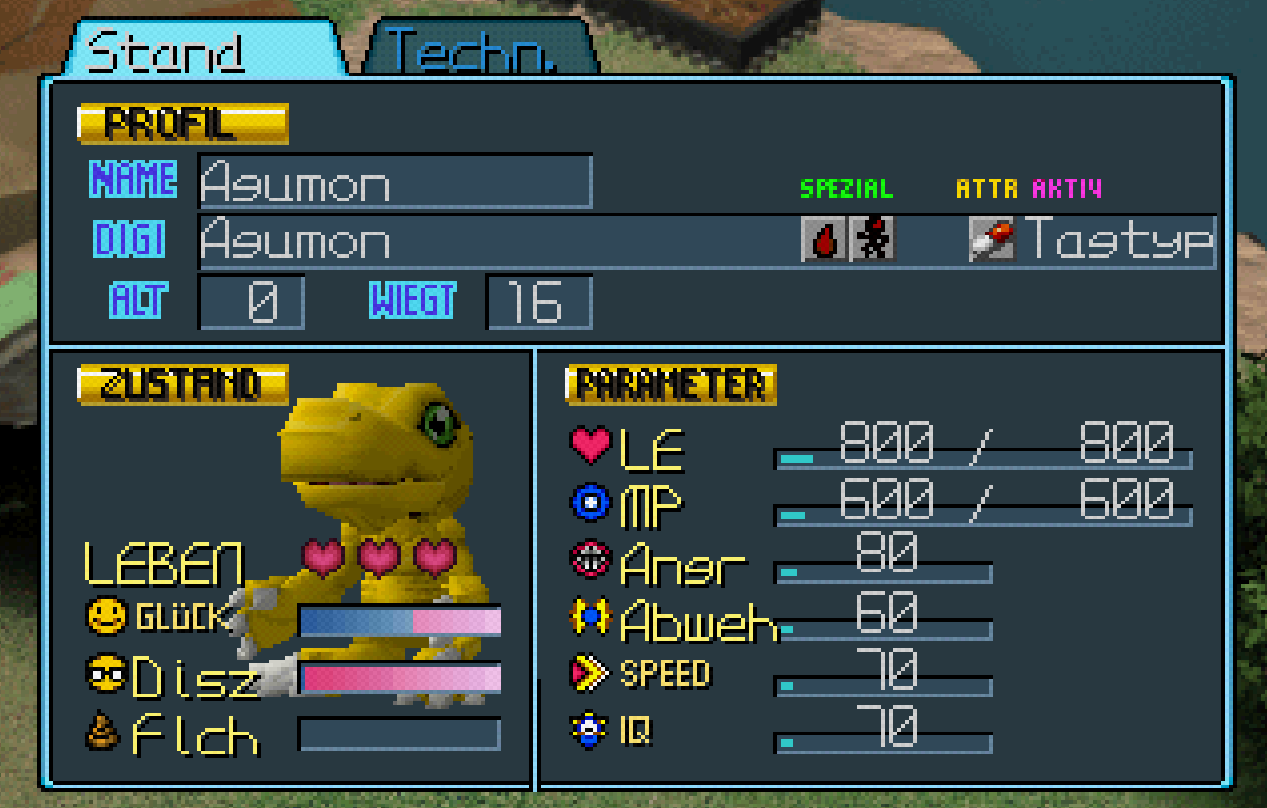
\includegraphics[width=0.8\columnwidth]{figures/screenshots/parameter.png}
    \caption{\label{fig:dw1-parameter} Digimon World: Statusmenü}
  \end{center}
\end{figure}

Das Partner-Digimon besitzt weitere Parameter, welche den aktuellen Status näher beschreiben.
Diese sind in \autoref{fig:dw1-parameter} in Zustand und Parameter unterteilt.
Das aktuelle Glück des Partners verändert seine Lebenserwartung.
Ist der Wert höher, lebt das Digimon länger.
Der Wert selbst kann durch Loben erhöht werden.
Allerdings sinkt dadurch die Disziplin.
Eine niedrige Disziplin kann dafür sorgen, dass ein Digimon Gegenstände verweigert.
Dazu zählen verschiedene Gegenstände, wie zum Beispiel Nahrungsmittel oder Gegenstände mit dauerhafter Wirkung.
Ein hoher Wert führt dazu, dass es eine kürzere Lebenserwartung hat.
Mithilfe der Tadeln-Funktion ist es möglich, diesen Wert zu erhöhen.
Allerdings verringert sich der Wert des Glücks, außer in zwei Ausnahmen.
Wenn das Digimon einen Gegenstand verweigert oder nicht in einer Toilette defäkiert.
In der US-Version des Spiels erhöht sich beim korrekten Tadeln das Glück zusätzlich. \\

Ein weiterer Teil von Digimon World sind Elemente aus Rollenspielen.
Dazu zählt die Entwicklung des Partner-Digimons, das Abschließen von Aufgaben (Quests) und echtzeitbasierte Kampfmechaniken.
Die Hauptquest des Spiels ist es, der Stadt einen bestimmten Wohlstand zu bringen und den letzten Gegner im Spiel zu besiegen.
Der Wohlstand wird erhöht, wenn ein Digimon in die Stadt eingeladen wird. Die Stadt erweitert sich schrittweise um bestimmte Funktionalitäten.
Beispielhafte Funktionen sind ein Gegenstandsladen, der Transport in andere Gebiete oder eine Klinik.\\

\begin{figure}[H]
  \begin{center}
    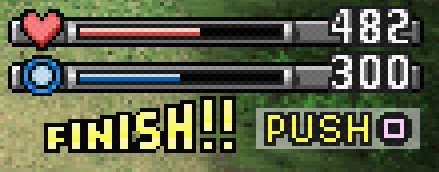
\includegraphics[width=0.7\columnwidth]{figures/screenshots/battle-parameter.png}
    \caption{\label{fig:dw1-battle-parameter} Digimon World: Lebens-, Magie- und Finisheranzeige}
  \end{center}
\end{figure}

Das Digimon besitzt Parameter, welche das Kampfgeschehen beeinflussen.
Die Lebens- und Magieanzeige gibt an, wie viel Leben oder Magie das Digimon aktuell im Kampf besitzt.
Diese sind in \autoref{fig:dw1-battle-parameter} zu sehen.
Der Angriffs- und Verteidigungswert beeinflussen die Schadensberechnung.
Der Code für diese Berechnung wurde auf Anfrage reverse engineered und hochgeladen\cite{calculatedamage}.
Die Formel für die Berechnung eines normalen Angriffs lautet

\begin{equation}
  \frac{T \cdot \frac{P + \frac{D \cdot P}{500}}{30} \cdot (RNG + 90)}{100}
\end{equation}

und kann durch Ausklammern und Umstellen vereinfacht werden:

\begin{equation}
  \frac{\frac{T}{30} \cdot  P \cdot (1 + \frac{D}{500}) \cdot (RNG + 90)}{100}
\end{equation}

Der Typ-Faktor $T$ bezeichnet den Wert, welcher aus der Summe von drei Spezialisierungen des Verteidigers gebildet wird.
Ein Typ beschreibt die im Spiel vorhandenen Elemente, wie zum Beispiel Feuer oder Luft.
Alle weiteren Spezialisierungen sind im Handbuch aufgelistet.
Der Anfgriffswert $P$ repräsentiert die rohe Kraft einer bestimmten Attacke.
$D$ wird berechnet durch die Differenz zwischen dem Angriffswert des Angreifers und dem Verteidigungswert des Verteidigers, wobei $D$ zwischen $-500$ und $500$ liegt.
Der Zufallsfaktor $RNG$ wird mithilfe der Funktion \texttt{random(21)} berechnet und befindet sich im Intervall $[0, 20]$.\\

Die Finisheranzeige in \autoref{fig:dw1-battle-parameter} lädt sich Schritt für Schritt anhand unterschiedlicher Wege im Kampf auf.
Dabei erscheinen schrittweise die Buchstaben, um das Wort \texttt{FINISH} auszuschreiben.
Der erste Weg ist, eine bestimmte Anzahl von Zeit im Kampf zu verbringen.
Ein weiterer Weg ist, einen Angriff erfolgreich auszuführen.
Zuletzt ist es möglich diese aufzuladen, wenn ein Angriff erfolgreich verteidigt wird.
Wenn die Finisheranzeige aufgeladen ist, kann die spielende Person diese mit der angezeigten Taste verbrauchen und einen besonderen Angriff auslösen.
Die Ausführung benötigt eine kurze Aufladezeit.
Wenn dieser Angriff beim Start unterbrochen wird, verfällt der besondere Angriff.
Ansonsten bleibt das gegnerische Digimon stehen und wartet, bis das Partner-Digimon den Angriff ausgeführt hat.
Während der Aufladezeit kann die spielende Person abwechselnd die Schultertasten \texttt{L1} und \texttt{R1} betätigen.
Die maximale Aufladung sind zehn Balken.
Für die maximale Aufladung benötigt die spielende Person 40 Tastenanschläge in $\approx 6$ Sekunden.
Diese Aufladung wird dann mit der rohen Angriffskraft und weiteren Faktoren multipliziert.\\

Eine Kampfsituation tritt ein, wenn der spielbare Charakter ein feindliches Digimon berührt.
Danach wird, anhand des aktuell sichtbaren Kamerasichtfelds, die Kampfzone initialisiert\cite{combat-asm}.
Jedes weitere feindliche Digimon, welches sich in einem gewissen Radius befindet, hat eine Chance dem Kampf beizutreten.
Der spielbare Charakter tritt zur Seite und der Kampf beginnt.
Der Kampf findet zwischen dem Partner-Digimon und $n$ feindlichen Digimon statt.
Zu Beginn des Spiels ist es nur möglich, die Optionen \texttt{Digimon vertrauen} oder \texttt{Flucht} auszuwählen.
Dabei ist es nicht möglich keine Option zu wählen.
Standardmäßig wird \texttt{Digimon vertrauen} am Anfang des Kampfes ausgewählt.
Digimon vertrauen bewirkt, dass das Digimon eigenständig handelt und sich wahlweise für unterschiedliche Angriffstechniken oder defensive Strategien entscheidet.
Flüchten bewirkt die Flucht aus dem Kampf und senkt Disziplin.
Es ist allerdings nicht möglich aus Kämpfen gegen Digimon, welche in die Stadt ziehen können, zu fliehen.\\

An dieser Stelle wird eine Kampfsituation, welche im Spiel vorkommen kann, näher erläutert.
Die Ausgangssituation ist, dass die spielende Person mit einem Agumon gegen Kunemon kämpft.
Agumon besitzt aufgrund vorheriger Kämpfe 649 von 800 Lebenspunkten und 450 von 600 Magiepunkten.
Das gegnerische Kunemon startet mit vollen Lebenspunkten.
Konkret sind dies 900 Lebenspunkte.
Der Kampf startet und die spielende Person wählt die Option \texttt{Digimon vertrauen} aus.
Danach läuft Agumon auf Kunemon zu und greift diesen mit der Technik \texttt{Feuerspeier} an, welche eine rohe Angriffskraft von 66 Punkten besitzt.
Ebenfalls kostet der Einsatz dieser Fähigkeit 30 Magiepunkte, weswegen Agumon nur noch 420 Magiepunkte besitzt.
Kunemon wehrt diesen Angriff allerdings ab, weswegen kein Schaden kalkuliert wird.
Agumon verwendet ein weiteres Mal \texttt{Feuerspeier} und fügt Kunemon 71 Schaden zu.
Der Rückstoß des Angriffs sorgt dafür, dass Kunemon zurückgestoßen wird.
Kunemon bewegt sich auf Agumon zu und versucht einen Nahkampfangriff auszuführen.
Allerdings unterbricht ein weiterer \texttt{Feuerspeier} diesen und Kunemon erleidet erneut 70 Schaden.
Das bedeutet, dass Kunemon nur noch 759 Lebenspunkte besitzt.\\

Nach einigen weiteren Angriffen besitzt Kunemon 262 und Agumon 286 Lebenspunkte.
Aus diesem Grund entscheidet sich die spielende Person, eine kleine Heildisk im Kampf zu verwenden, welche 500 Lebenspunkte heilt.
Agumon besitzt dank dieser Heildisk wieder 786 von 800 Lebenspunkten.
Während des Kampfes hat sich ebenfalls die Finisheranzeige aufgeladen.
Die spielende Person entscheidet sich, diese aufzubrauchen und Agumon startet die Technik \texttt{Pfeffer + Salz}, welche 89 rohen Angriffsschaden verursacht.
Die spielende Person betätigt die Schultertasten abwechselnd so schnell wie möglich, aber schafft es nur neun der zehn Balken aufzufüllen.
Agumon verwendet die Technik und fügt Kunemon 366 Schaden zu.
Kunemon sinkt dadurch auf null Lebenspunkte und der Kampf endet. \\

Die Anzahl an Optionen den Kampf zu manipulieren steigt mit einem höheren Intelligenzwert.
Bei einer Intelligenz von 100 ist es möglich, dem Partner zu befehligen, immer den stärksten Angriff zu verwenden.
Ein Wert von 200 bewirkt das Gegenteil und der Partner verwendet immer den schwächsten Angriff.
Dies kann nützlich sein, wenn man die Magiepunkte langsamer aufbrauchen möchte.
Die Möglichkeiten defensiver zu spielen, werden bei einem Wert von 300 und 400 freigespielt.
Ab diesem Zeitpunkt ist möglich, dem Partner zu befehligen, auzuweichen oder zu verteidigen.
Ebenfalls wird die Option freigeschaltet, manuell den Fokus zwischen mehreren Gegner zu wechseln.
Ab einem Intelligenzwert von 500 werden die beiden Optionen, welche bei 100 und 200 freigeschaltet wurden, durch die verfügbaren Kampffertigkeiten ersetzt.
Der letzte Wert von 999 erweitert das Repertoire an Optionen nicht, allerdings senkt dieser die Kosten für die Verwendung von Kampffertigkeiten.
Das Erlernen von neuen Kampffertigkeiten erfolgt entweder anhand eines höher erreichten Intelligenzwertes oder zufällig im Kampf.
Die Wahrscheinlichkeiten, eine Fertigkeit zu Erlernen, sind mithilfe eines Tools einsehbar\cite{move-tool}. \\

\begin{figure}[H]
  \begin{center}
    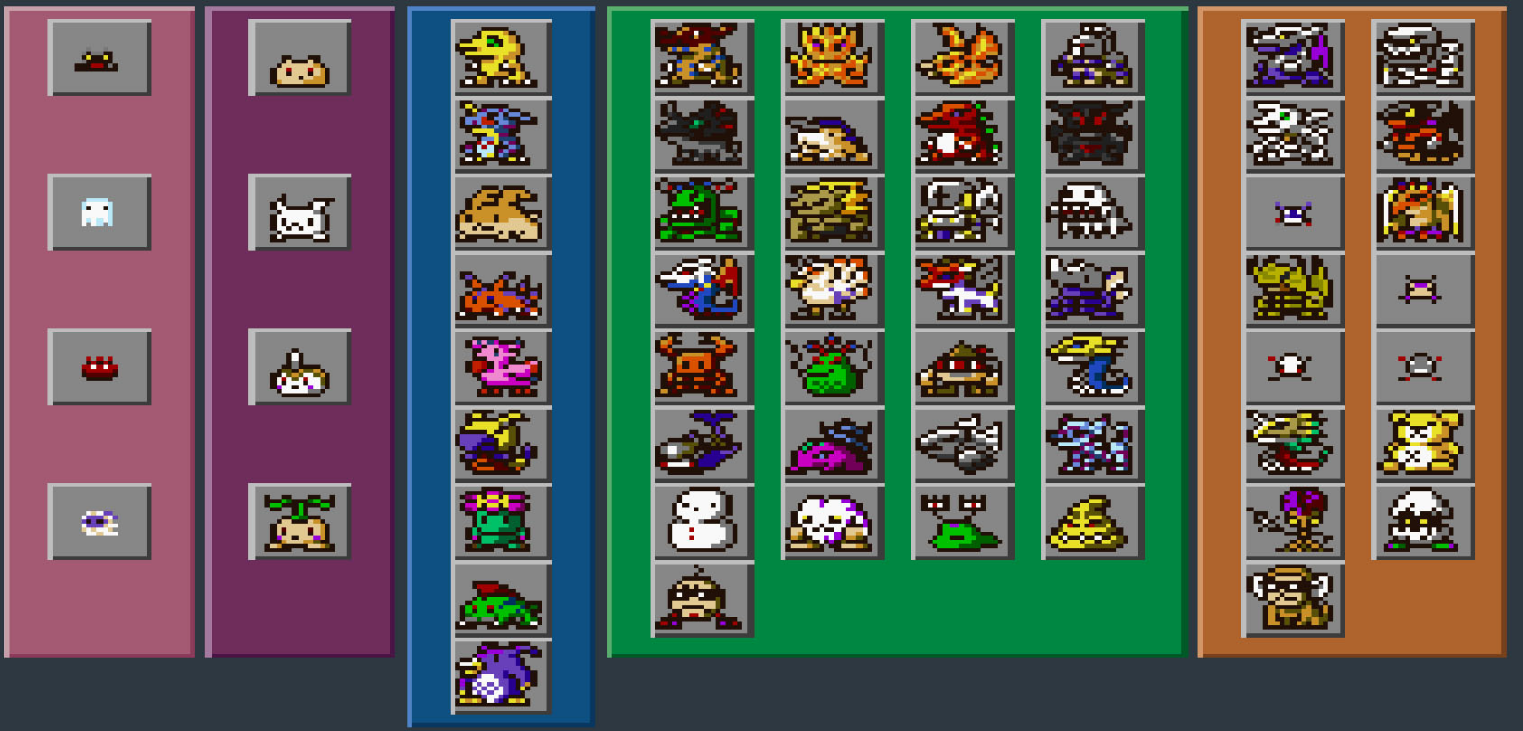
\includegraphics[width=1\columnwidth]{figures/screenshots/digivolutions.png}
    \caption{\label{fig:dw1-digivolutions} Digimon World: Alle Entwicklungsformen}
  \end{center}
\end{figure}

Digimon World beinhaltet eine bestimmte Form der Entwicklung.
Diese nennt sich Digitation und ist Hauptbestandteil des Digimon-Universums.
Diese wird auch im Handbuch des Spiels beschrieben.
Digimon durchlaufen verschiedene Entwicklungsstufen, welche in \autoref{fig:dw1-digivolutions} zu sehen sind.
Das Handbuch beschreibt die Entwicklung vom Ausbildungs- bis zum Ultralevel.
Allerdings wird das Babylevel außer Acht gelassen, welches sich noch vor dem Ausbildungslevel stattfindet.
Die Digitation findet nach einer bestimmten Zeitspanne statt und richtet sich dann nach bestimmten Kriterien.
Die Kriterien basieren auf Parametern, wie zum Beispiel Angriffswerten oder Intelligenz, dem aktuellen Gewicht, Pflegefehler und unter Umständen einem Bonuskriterium.
Mithilfe eines Tools lassen sich diese Kriterien besser nachverfolgen\cite{digivolution}. \\

Es existieren verschiedene Gegenstände, welche Werte des Partners verändern können.
Disks können im und außerhalb des Kampfes verwendet werden und helfen, Kampfparameter wie Lebens- oder Magiepunkte aufzufüllen.
Chips sind Gegenstände, welche die maximale Obergrenze von Parametern erhöhen können.
Diese Wirkung ist permanent.
Nahrungsmittel füllen die Hungerleiste des Digimons wieder auf und besondere Gegenstände wie das Camping-WC sorgen dafür, dass die Toilette überall verwendet werden kann.
Zuletzt gibt es noch Gegenstände, welche eine Digitation erzwingen können.
Einzelne Gegenstände werden auch in den Handbüchern beschrieben, allerdings fehlen viele Abbildungen in der deutschen Ausgabe.\\

Neben den zahlreichen Gegenständen ist es auch möglich, die Werte durch Digitation, Kämpfe oder Training zu erhöhen.
Die gerade beschriebenen Gegenstände, welche eine Digitation erzwingen, erhöhen die Werte allerdings nicht.
Das bedeutet, dass es effizienter ist, das Parnter-Digimon ohne Gegenstände zu einem höheren Digitationslevel zu entwickeln.
Das Spiel bietet zusätzlich viele verschiedene Trainingsareale, welche helfen, die Werte des Partner-Digimons zu erhöhen.
Konkrete Informationen zum Training können mithilfe eines Tools berechnet werden\cite{dw-training}.
Durch Kämpfe ist es ebenfalls möglich, an höhere Werte zu kommen.
Allerdings sind diese im Vergleich zum Training wenig effizient.\\

Im Spiel existieren noch weitere Funktionen, wie das Sammeln von Karten, Medaillen oder das Bestreiten von Turnieren.
In den Turnieren kann der Kampf mithilfe der Memory Card\footnote{Speicherkarte für die \ac{PSX}} gegen eine weitere Person ausgetragen werden.
Allerdings werden diese Funktionen in der Bachelorarbeit bewusst nicht berücksichtigt.
Das liegt daran, dass diese Funktionalitäten nicht relevant für den Prototypen und das fertige Produkt sind.\\
\subsection{Unterschiede zwischen den Versionen}
% PAL vs NTSC
Ein regionaler Unterschied zwischen den Versionen liegt im Bildübertragungsverfahren.
Europäische Versionen des Spiels verwenden das \ac{PAL}-Verfahren und andere Versionen das \ac{NTSC}-Verfahren.
Im Vordergrund steht die unterschiedliche Hertz-Anzahl dieser Verfahren.
Dabei unterstützt  \ac{PAL} ein vielfaches von 50 und \ac{NTSC} ein vielfaches von 60 Hertz\cite{pal-vs-ntsc}.
Die Hertzangabe ist in diesem Fall ausschlaggebend dafür, wie oft pro Sekunde der Fernseher Einzelbilder rendern kann.\\

% PAL Bug
Aufgrund eines Fehlers in der \ac{PAL}-Version ist es in einigen Ausgaben des Spiels nicht möglich, das Spiel durchzuspielen.
Der Fehler verhindert den Zugang zu Ogremons Festung und das Betreiben des Aufzugs im Berg der Unendlichkeit\cite{epicplay}.
Beide Inhalte sind elementarer Bestandteil der Story und nötig, um das Spiel durchzuspielen.
Die \ac{NTSC}-Version enthält ebenfalls mehrere Fehler, welche zum Einfrieren des Spiels führen können\cite{gamefaqglitch}.
Allerdings verhindern diese nicht die Komplettierung des Spiels.\\

\begin{figure}[H]%
    \centering
    \subfloat[\centering Schatten]{{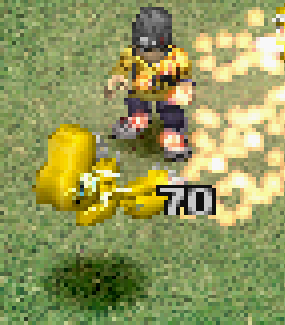
\includegraphics[width=4cm]{figures/screenshots/shadow.png}
                \label{fig:dw1-shadow-a}}}%
    \qquad
    \subfloat[\centering Echtzeitschatten]{{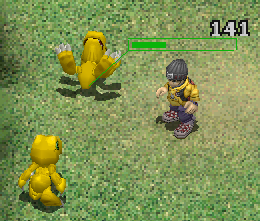
\includegraphics[width=7cm]{figures/screenshots/korean.png} }\label{fig:dw1-shadow-b}}%
    \caption{Unterschiedliche Methodiken zur Schattierung von Objekten}%
    \label{fig:dw1-shadow}%
\end{figure}

% PC Version
Zusätzlich ist das Spiel im April 2002 in Korea für den PC erschienen\cite{korea-multi}.
Im Vergleich zu der \ac{PSX}-Version existieren zwei nennenswerte Unterschiede.
Zum einen ist es möglich das Spiel an jeder beliebigen Position zu speichern, zum anderen werden Echtzeitschatten von Charakteren gerendert.
Dies ist deutlich in \autoref{fig:dw1-shadow-b} zu sehen.
Einige Texturen sind ebenfalls hochauflösender.\\

Aufgrund der Tatsache, dass die Verkaufszahlen allerdings nur $\approx 6{,}15\%$ der gesamten Verkaufszahlen ausmachen und einige Unterschiede zu der \ac{PSX}-Version existieren, wird die PC-Version kein zentraler Bestandteil der Untersuchung sein\cite{vgchartz}.
Die \ac{PSX}-Spiele wurden zusammen mit einem Handbuch für das Spiel verkauft.
Im Anhang der Arbeit befinden sich die Handbücher in japanischer, amerikanischer und deutscher Fassung.
Die Handbücher und einige Unterschiede werden im \autoref{sec:game-content} vorgestellt.\\

\newpage
\section{Ist-Analyse}\label{sec:ist}
In den folgenden Unterabschnitten wird der Ist-Zustand des Spiels näher beleuchtet\cite{grundlagen-grochla}. Die Abschnitte beschreiben Vorgänge, welche die aktuelle Ausganslage analysieren. Der Ist-Zustand ist eine wertungsfreie Momentaufnahme, welche Voraussetzung für die Soll-Analyse in \autoref{sec:soll} ist\cite{ist-zustand}. Die erhobenen Daten werden verwendet, um Lösungsansätze für erkannte Problematiken zu entwickeln. 
\subsection{Rezensionen}
Insgesamt scheint Digimon World ein mittelmäßiges Spiel zu sein. Die durchschnittliche Bewertung des Spiels von $52{,}55\%$ verdeutlicht dies\cite{metacritic-gamerankings}. In erster Linie wird das Kampfsystem stark kritisiert. Es gibt nur wenige Möglichkeiten im Kampf zu agieren und das Resultat wird nur durch das vorherige Training entschieden\cite{ign}. Der Kampf wird mehr als eine Art Beobachtung beschrieben und nicht als rentabel angesehen. Ebenfalls wird vermutet, dass sich das Spiel primär an Fans von Digimon richtet\cite{gamespot}. 
\subsection{Fragebogen in Amerika}
Die amerikanische Version von Digimon World beinhaltet einen Fragebogen in der CD-Hülle. Dieser erfasst demografische Daten und Kritik zum Spiel. Weiterhin ist das Briefporto für den Rücksand des Fragebogens bereits bezahlt. Aus diesem Grund ist davon auszugehen, dass die Rücklaufquote entsprechend höher ist. Aufgrund dieser Tatsache wurde die Pressestelle von Bandai Namco kontaktiert und darum gebeten, die Auswertung der Statistik für die Bachelorarbeit bereitzustellen. Allerdings teilte der Senior PR-Manager von Bandai Namco\footnote{Marco Süß ist seit 2016 PR-Manager bei Bandai Namco\cite{marcosuess}} mit, dass ein Zugriff und die Herausgabe der Daten nicht möglich sei.

\subsection{Interviews}\label{sec:interview}
Die Arbeit bedient sich der empirischen Methode des kontextuellen Interviews\cite{contextual-design}.
Diese wird in der nutzungsorientierten Gestaltung verwendet, um ein Produkt im realen Nutzungskontext zu untersuchen.
Ziel dieser Vorgehensweise ist es, externe Einflüsse in einem Interview mit einzubeziehen und zu verstehen.
Die Ausführung dieser Methodik wird in Form eines Leitfadeninterviews\cite[S.559 ff.]{handbuch-methoden-der-empirischen-sozialforschung}\cite[S. 121 ff.]{methoden-in-der-naturwissenschaft} gestaltet.
Die aus diesem Verfahren generierten qualitativen Daten werden verwendet, um neue Hypothesen zu entwickeln.
Diese werden im Anschluss in \autoref{sec:survey} anhand einer Umfrage überprüft.\\

Damit unterschiedliche Ansichten abgedeckt werden, werden drei verschiedene Testpersonen für diese Methodik ermittelt.
Die Befragung wird in Einzelgesprächen durchgeführt, um jeder Person mehr Zeit zu geben, über einzelne Themen zu berichten\cite[S.95]{game-research-methods}.
Der entwickelte Interviewleitfaden (siehe Anhang \autoref{table:interview-guideline}) weist den Fragen in der Kategorie \textit{Beobachtung} keine spezifische Reihenfolge zu.
Das liegt daran, dass diese Fragen situativ gestellt werden.
Ebenfalls kann es sein, dass gewisse Situationen nicht entstehen und diese Fragen ausgelassen werden.
Da es sich um einen Leitfaden handelt, können auch zusätzliche oder weniger Fragen gestellt werden.\\

\begin{figure}[ht]
  \begin{center}
    
\includegraphics[width=1\columnwidth]{figures/interview-workflow.pdf}
    \caption{\label{fig:interview-workflow} Interviewprozess}
  \end{center}
\end{figure}

\autoref{fig:interview-workflow} verdeutlicht die vier Phasen, welche in einem Interview realisiert werden.
In der Einleitungsphase wird den Versuchspersonen der Interviewprozess erklärt.
Auf diese Art und Weise kann sich die Person besser auf das Vorgehen und die Ziele konzentrieren.
Ebenfalls werden Eingangsfragen gestellt, um demografische Daten zu erfassen.
Die Warm-Up-Phase dient dazu, die Testpersonen auf die Beobachtungsphase vorzubereiten.
Dies soll das Interviewklima mit einfachen Fragen auflockern\cite{methods-of-data-collection}.
In der Beobachtungsphase wird die Person aufgefordert, das untersuchte Spiel Digimon World zu spielen.
Die beobachtende Person hilft in dieser Phase des Interviews an keiner Stelle mit eigener Erfahrung oder bei Fehlern aus.
Dies ist wichtig, da ansonsten die Testperson in ihren Aktionen beeinflusst werden könnte.
Fragen in dieser Phase werden verstärkt als Impulse zur Anregung eines Gesprächs verwendet und folgen dem Motto: \glqq So offen wie möglich, so strukturierend wie nötig\grqq{}\cite[S. 563]{handbuch-methoden-der-empirischen-sozialforschung}\cite[S. 126]{methoden-in-der-naturwissenschaft}.
Die befragende Person, kann in der Abschlussphase, aufgetretene Probleme oder Wünsche der befragten Person ansprechen.
Diese Phase ist primär zur Diskussion von Lösungsansätzen gedacht.
Zusätzlich hilft diese Phase falsch verstandene Informationen oder Interpretationen zu berichtigen.
Es ist wichtig, dass die falsch verstandenen Informationen oder Interpretationen nicht in der Beobachtungsphase angesprochen werden, weil dies die befragte Person ebenfalls beeinflussen könnte.\\

Die Auswahl der Testpersonen erfolgt anhand zwei unterschiedlicher Kriterien.
Die Erfahrung mit dem Spiel Digimon World und das Geschlecht der Testperson.
Die Erfahrung soll Aufschluss darüber geben, wie stark sich die Spielweise von einer Person mit keiner Erfahrung gegenüber einer Person mit viel Erfahrung unterscheidet.
Diverse Studien zeigen, dass auch das Geschlecht in Videospielen ausschlaggebend für die Fähigkeiten oder Präferenzen der Spielenden sein kann.
Männliche Versuchsteilnehmer verfügen, im Vergleich zu weiblichen Teilnehmerinnen, über stärker ausgeprägte Fähigkeiten in der räumlichen Navigation\cite{gender-maze}\cite{gender-shopping}.
Im Kontrast dazu legen weibliche Teilnehmerinnen, im Vergleich zu männlichen Teilnehmern, einen größeren Fokus auf das Aussehen des Charakters\cite{gender-items-in-mmo}\cite{gender-clothes}.\\

Der Versuchsaufbau findet in der Wohnung der jeweiligen Testperson statt.
Der Grund dafür ist, dass dies Vertrautheit und ein angenehmeres Klima für die befragte Person schaffen soll.
Ebenso können in dieser Umgebung kontextabhängige Probleme erkannt werden.
Bevor das Interview startet, wird der Testperson eine Playstation mit dem Spiel Digimon World überreicht.
Schließlich werden die einzelnen Prozesse anhand des Interviewleitfadens durchlaufen.
Die Beobachtungsphase wird jeweils nach zwei Stunden beendet, da längere Spielphasen zu ermüdend für die teilnehmende Person wären.
Das Interview wird mit einem Mikrofon aufgenommen.
Danach werden wörtliche, nicht lautsprachliche, Transkripte angefertigt.
Die Methode der Audiotranskription bietet den Vorteil, dass einzelne Passagen einfacher in einem Text referenziert werden können.
Ebenso können die erfassten Daten auf diese Art und Weise anonymisiert und pseudonymisiert werden.
Das bedeutet nicht, dass die einzelnen Texte bestimmten Personen zugeordnet werden können und die Daten durch ein Kennzeichen ersetzt sind\cite[S.97]{game-research-methods}.

\begin{center}
  \begin{table}[!ht]
    \begin{tabular}{ l | c | c | c }
                               & P1            & P2               & P3            \\
      \hline
      \hline
      Alter                    & 23            & 21               & 24            \\
      Geschlecht               & \male         & \female          & \male         \\
      Präferenz Peripherigerät & Spielabhängig & Maus \& Tastatur & Spielabhängig \\
      Gerät für Videospiele    & PC            & PC               & PC            \\
      Tamagotchi               & \xmark        & \xmark           & \cmark        \\
      Digimon                  & \xmark        & \xmark           & \cmark        \\
    \end{tabular}
    \caption{Zusammenfassung der Antworten auf die Einleitungsfragen}
    \label{table:interview-results}
  \end{table}
\end{center}

\autoref{table:interview-results} veranschaulicht zusammengefasst die Antworten der Testpersonen auf die Eingangsfragen.
Diese Daten werden in \autoref{sec:survey} verwendet, um einen Umfragebogen zu gestalten.
Die Referenzen sind hierbei mit [Px, Z. y] bezeichnet, wobei x die befragte Person und y die entsprechende(n) Zeile(n) referenziert.
Ebenfalls sollen im Transkript vorkommende Hypothesen konstruiert werden, welche gleichermaßen in diesen Fragebogen einfließen.
Diese sind mit [Hx] bezeichnet, wobei x die entsprechende Hypothese darstellt.\\

% Kulturelle Unterschiede
Während des Interviews fällt auf, dass einige Spielelemente missverständlich für den westlichen Markt sind.
Person 1 läuft mehrmals an einer Toilette vorbei, ohne diese als solche identifizieren zu können.
Das liegt daran, dass  in Digimon World am Einstiegspunkt eine japanische Hocktoilette, anstelle einer westlichen Sitztoilette, platziert ist.
Person 2 kann diese hingegen als solche identifizieren[P2, Z.732-738].
Allerdings existieren bei Person 2 Schwierigkeiten, das Kreis- und Kreuzsymbol in Centauromons Minispiel korrekt zu interpretieren[P2 Z.826f].
Diese Fehlinterpretation lässt auf kulturelle Unterschiede zurückführen, da im japanischen ein Kreis-Symbol (\begin{CJK}{UTF8}{min}まる\end{CJK}) eine korrekte Aussage und ein X-Symbol (\begin{CJK}{UTF8}{min}ばつ\end{CJK}) eine falsche Aussage symbolisiert\cite{intermediate-japanese}.
Im westlichen Markt hingegen wird das X-Symbol zum Beispiel verwendet, um Kontrollkästchen auszufüllen oder als Ziel in Schatzkarten\footnote{Redewendung: \glqq Das X markiert die Stelle\grqq}.
Dies spiegelt sich auch im Design der Playstation-Controller wieder.
In der japanischen Region werden Spielinhalte mit der O-Taste, in der westlichen Region der Welt hingegen mit der X-Taste bestätigt\cite{controller-japanese}.
Die positiv assozierte Verknüpfung ist auch im japanischen Handbuch des Spiels auf Seite 19 deutlich zu sehen.
Die Tatsache, dass ein Spiel in unterschiedlichen Regionen der Welt missverstanden werden kann, wird in dieser Arbeit allerdings bewusst nicht als Hypothese thematisiert.
Das liegt daran, dass das Ermitteln der Problematiken im Optimalfall mit verschiedenen Personen aus der ganzen Welt besprochen werden muss.
Dies würde allerdings viel Zeit in Anspruch nehmen und wird aus diesem Grund zunächst vernachlässigt.\\

% Entwicklungsstufen und Identifikation von Protagonisten
Es ist aufgefallen, dass Probleme bei zwei der drei Testpersonen auftreten, weil diese bisher keine Berührungspunkte mit Digimon hatten.
Eines dieser Probleme ist, dass die Testpersonen kein Verständnis für die einzelnen Entwicklungsstufen aufzeigen können.
Dies ist problematisch, weil das Verständnis dafür fehlt, dass das Starter-Digimon sich abhängig der aktuellen Parameter, zum Zeitpunkt der Entwicklung, entwickelt.
Im Kontrast dazu steht für die Testpersonen die, bis auf wenige Ausnahmen, lineare Entwicklung in Pokémon[P1, Z.433-435].
Ein weiteres Problem ist, dass durch den mangelnden Berührungspunkt mit Digimon die Hauptquest nicht vollständig wahrgenommen werden kann.
Digimon, welche in die Stadt eingeladen werden sollen, können dabei nicht als solche identifiziert werden[P1, Z. 255-257].
Ein Beispiel hierfür ist das Digimon Agumon, welches aus der Serie Digimon Adventure als Protagonist bekannt ist.
Dieses Digimon existiert im Spiel ein einziges Mal und alle weiteren Vorkommen von Agumon im Spiel sind alternative Abwandlungen\footnote{Zum Beispiel SnowAgumon, welche eine weiße anstelle einer gelben Färbung der Haut besitzen oder ToyAgumon, welche gänzlich aus Klemmbausteinen bestehen}, welche häufiger vorkommen.
Person 3 kann diese, dank ihres bestehenden Wissens über das Digimon-Universum, jedoch voneinander unterscheiden[P3, Z. 1258-1261].\\

% Aufgabenliste
Aufgrund dieser Probleme ist die Idee aufgekommen, dass eine Aufgabenliste vorteilhaft wäre\hypothesis[P1, Z. 533].
Die Kernaufgabe befindet sich zwar im Hinterkopf der befragten Personen, allerdings scheint diese zu breit gefächert[P1, Z. 527-531].
Die Aufgabenliste soll dazu beitragen, die Kernaufgaben in kleinere Unteraufgaben zu unterteilen.
Auf diese Art und Weise können die gesuchten Digimon näher in der Aufgabenliste beschrieben und anschließend identifiziert werden.
Diese Art der Aufgabenliste ist zwar in Form mehrerer \ac{NPC} in der Stadt vorhanden, allerdings geben diese nur grobe Richtungen vor.
Genauso könnte die neue Aufgabenliste permanent abrufbereit sein. Die Aufgabenliste soll ebenfalls davor schützen, dass die Spielenden sich nicht überfordert fühlen[P1, Z. 49-51].\\

% Mangelnde Details und Fortschrittsbalken
Mangelnde Details oder fehlende Informationen werden mehrmals in den Interviews erwähnt.
Einige Gegenstände besitzen keine konkreten Werte, sondern grobe Beschreibungen\footnote{Die Beschreibung für Fleisch oder einen Digipilz lautet: \glqq Nahrung. Sättigt Digimon etwas.\grqq}[P1, Z. 80 f.].
Aus diesem Grund wird die Hypothese aufgestellt, dass Gegenstände im Spiel konkrete Werte benötigen\hypothesis[P1, Z. 143 f.][P3, Z. 1315 f.].
Ebenfalls soll ein Fortschrittsbalken für den Nahrungs- oder Toilettenbedarf der Planung der spielenden Person entgegenkommen\hypothesis[P1, Z. 230 f.].
Diese Hypothese wird von Person 2 durch die Aussage gestützt, dass Forderungen oftmals zu spät erscheinen[P2, Z. 886-888].
Die im Spiel vorkommenden Fortschrittsbalken sind für die befragten Personen irreführend.
Das liegt daran, dass die Fortschrittsbalken aus jeweils zwei Fortschrittsbalken bestehen.
Damit ein Digimon maximale Disziplin erlangen kann, muss sich der Balken folglich zwei Mal füllen.
Dieses System wird von allen Teilnehmenden kritisiert oder missverstanden[P1, Z. 186-188][P2, Z. 850-854][P3, Z. 1094-1100].
Daraus lässt sich die Schlussfolgerung ziehen, dass die angezeigten Fortschrittsbalken nicht unterteilt werden sollten\hypothesis. \\

% Mehr Informationen im HUD
Die befragten Personen wünschen sich ebenfalls mehr oder klarer kommunizierte Informationen im \ac{HUD}.
Dazu zählen weitere Fortschrittsbalken, wie zum Beispiel ein weiterer Lebensbalken oder Fortschrittsbalken, welche in H3 erwähnt wurden\hypothesis[P2, Z. 750-754][P3, Z. 1160-1173][P3, Z. 1245-125].
Im Fall, dass das Partner-Digimon im Kampf verliert, gehen Gegenstände verloren.
Um welche Gegenstände es sich handelt, wird allerdings nicht kommuniziert[P2, Z. 748-752].
Damit die spielende Person sich die Items im Inventar nicht dauerhaft merken muss, könnte es von Vorteil sein, die verlorenen Items aufzulisten\hypothesis.
Beim Interview mit Testperson 1 ist aufgefallen, dass nicht ganz klar war, wie viel Zeit beim Training vergeht.
Es wird die Frage gestellt, ob ein Indikator in Form einer Animation dies deutlicher machen könnte\hypothesis.
Diese Frage wird bejaht[P1, Z. 282-286]. Das \ac{HUD} sollte anzeigen, mit welchen Tasten Aktionen ausgeführt werden.
Auf diese Art und Weise können Aktionen von Spielenden nicht nur durch das Drücken zufälliger Tasten erlernt werden\hypothesis[P1, Z. 59-62][P3, Z. 1000-1009][P3, Z. 1113-1116].
Die Uhr im \ac{HUD} scheint die befragten Personen ebenfalls zu verwirren[P1, Z. 99-103][P3, Z. 1033-1042].
Das liegt daran, dass im Spiel einer der beiden Zeiger einer 12-Stunden-Uhr durch einen Punkt ersetzt wurde.
Dieser Punkt sollte allerdings ein Zeiger sein, damit Spielende die Uhr einfacher mit einer realen Uhr vergleichen können\hypothesis.\\

% Entfernen vom Tadeln
Das Tadeln und der Fortschrittsbalken für die Disziplin wird ebenfalls missverstanden.
Das Spiel beinhaltet eine Mechanik, dass sich das Partner-Digimon abhängig von der Disziplin dazu entscheiden kann, einen Gegenstand abzulehnen.
Der korrekte Ansatz wäre, das Partner-Digimon für das Verweigern zu tadeln.
Dadurch erhöht sich die Disziplin und das Partner-Digimon lehnt den Gegenstand nicht mehr ab.
Eine der am Interview teilnehmenden Personen scheint keinen Sinn darin zu sehen, das Digimon zu tadeln[P1, Z. 457-463].
Eine weitere Person scheint nur Partner zu tadeln, welche schlechter als andere Partner waren[P3, Z. 1101-1106] oder um bestimmte Parameter zu verändern[P3, Z. 1251-1257].
Ebenfalls erscheint diese Funktion den Spielenden Inhalte des Spiels zu verwehren.
Weder können Basisfunktionen, wie zum Beispiel das Füttern eines Digimons[P2, Z. 708-711], noch erweiterte Funktionen, wie zum Beispiel das Nutzen von Medizin, Disks oder Chips[P1, Z. 322-331][P1, Z. 479-499], verwendet werden.
Aus diesem Grund kann auf diese Funktion gänzlich verzichtet werden\hypothesis.\\

% Karte
Personen, welche im Interview erste Erfahrungen mit dem Spiel sammeln, haben Schwierigkeiten, sich in der Spielwelt zu orientieren[P1, Z. 109 f.][P1, Z. 444-446][P2, Z. 760-762].
Allerdings finden diese Testpersonen ebenfalls eine Lösung für das Problem.
Eine Karte soll helfen, die aktuelle Position in der Spielwelt zu markieren\hypothesis[P1, Z. 172-175][P1, Z. 521-524][P2, Z. 765].
Diese sollte in Form einer Minimap\footnote{Verkleinerte Darstellung der Karte im \ac{HUD}}, aber auch im Menü aufzufinden sein[P2, Z. 767 f.].
Die Karte soll allerdings nicht nur das Terrain, sondern auch Informationen über Nahrungspunkte[P2, Z.798] oder verfügbare Toiletten[P1, Z. 129 f.][P2, Z. 810-813] anzeigen\hypothesis.\\

% Geschlecht und Charaktererstellung
Die Annahme, dass das Geschlecht ausschlaggebend für eine andere Sicht auf das Spiel sein kann, wird im Interview bestätigt.
Die Teilnehmerin P2 erläutert, dass es störend sei, dass das Geschlecht am Anfang des Spiels nicht auswählbar ist[P2, Z. 651-655].
Dadurch entsteht das Gefühl, dass die Zielgruppe nur männliche Spieler sind[P2, Z. 658-660].
Das in dieser Arbeit geplante Spiel soll allerdings eine breiter gefächerte Zielgruppe ansprechen.
Aus diesem Grund soll den Spielenden die Option gegeben werden, das Geschlecht anzupassen\hypothesis.
Ebenfalls kann in Betracht gezogen werden, dass einzelne Anpassungen am Aussehen des Charakters vorgenommen werden können\hypothesis[P2, Z. 665-668]. \\

% Kampfsystem
Der Interviewleitfaden in \autoref{table:interview-guideline} hebt, in der Abschlussphase des Interviews, das Kampfsystem hervor.
Dabei stellte sich die Frage, inwieweit Spielende Einfluss auf das Kampfgeschehen nehmen sollen.
Die Testpersonen wünschen sich bereits am Anfang des Spiels mehr Möglichkeiten in das Kampfgeschehen einzugreifen\hypothesis[P1, Z. 572-601][P2, Z. 898-901][P3, Z. 1336-1343].
Eine mögliche Umsetzung ist der von Person 2 genannte rhythmusbasierte Kampf[P2, Z. 817-819][P2, Z. 902-904].
Die Frage, auf welche Art und Weise diese Hypothesen umgesetzt werden sollen, bleibt allerdings zunächst offen und wird in einem späteren Kapitel näher behandelt.

% Tutorial
Bei Betrachtung der gerade genannten Hypothesen wird deutlich, dass den Spielenden überwiegend Informationen fehlen.
Einige dieser Informationen sind im Handbuch des Spiels enthalten.
Zwei der drei befragten Personen haben sich das Handbuch allerdings nicht angesehen.
Dies kann mehrere Gründe haben.
Zum einen kann es sein, dass Testpersonen dies nicht als Aufgabe des Versuchsaufbaus betrachtet haben, zum anderem könnte es sein, dass die befragten Personen ein Tutorial\footnote{Gebrauchsanleitung} im Spiel erwartet haben.
Das im Spiel implementierte Tutorial verlangt, dass die Spielenden die einzelnen \ac{NPC} in der Stadt ansprechen.
Allerdings kann es passieren, dass Spielende zunächst kein Interesse zeigen diese anzusprechen und das Erkunden der Umgebung priorisieren[P1, Z. 51-53][P1, Z. 112-119].
Die Konsequenz aus dieser Design-Entscheidung ist, dass Spielende beim Erkunden auf Grundfunktionen verzichten müssen, da diese im Spiel nicht erklärt wurden[P1, Z. 58-75][P2, Z. 695-696][P2, Z. 719-721][P2, Z. 832-834][P2, Z. 891-893].
Zusammenfassend lässt sich sagen, dass ein Tutorial den Spielenden helfen kann, Grundfunktionen zu erlernen\hypothesis.


\subsection{Umfrage}\label{sec:survey}
Die in \autoref{sec:interview} aufgestellten Hypothesen werden in diesem Kapitel näher untersucht.
Die empirische Methode der Online-Umfrage\cite{value-online-survey} ermöglicht es, die im Interview ermittelten Daten zu quantifizieren.
Die Aussagekraft einer Online-Umfrage ist vergleichbar mit Papier-Bleistift-Befragungen\cite{online-marktforschung}.
Mithilfe der quantitativen Daten können, anhand von Methoden der statistischen Analyse, neue Erkenntnisse erschlossen werden.
Die Stichprobe wird innerhalb mehrerer Discord\footnote{Ein soziales Medium, welches Personengruppen in Server unterteilt\cite{discord}}-Server durchgeführt.
Jede Person auf dem Discord-Server besitzt die gleiche Wahrscheinlichkeit an der Online-Umfrage teilzunehmen und somit Teil der Stichprobe zu sein.
Das Auswahlverfahren erfolgt also zufällig.
Diese Server richten sich primär an Personen, welche ein Interesse an Digimon-Videospiel Remakes\footnote{Ein Remake beschreibt in diesem Kontext die Anpassung eines Videospiels zum Zweck der Modernisierung.} oder Digimon im Allgemeinen aufweisen.
Aus diesem Grund kann die Wahrscheinlichkeit, dass eine Person Kontakt mit Digimon World hat, höher sein.
Die Umsetzung der Online-Umfrage versichert auch, dass die erhobenen Daten anonymisiert sind.\\

Der Aufbau des Fragebogens gliedert sich in drei Teile.
Der erste Teil der Umfrage erhebt demografische Daten und lockert mit einfachen Eingangsfragen die Umfrage auf.
Dies erfolgt analog zu den ersten beiden Phasen des Interviewleitfadens aus \autoref{table:interview-guideline}.
Der zweite Abschnitt ermittelt allgemeine Informationen zum Spiel.
Diese Informationen geben in der statistischen Analyse Aufschluss darüber, inwiefern unterschiedliche Nutzergruppen die einzelnen Hypothesen bewerten.
Ebenfalls beinhaltet die Umfrage zwei Freitext-Felder, um weitere qualitative Daten bezüglich des Kampfsystems zu erfassen.
Dieses Feedback wird in der späteren Implentierungsphase berücksichtigt.
Abschließend bewerten die Teilnehmenden im letzten Teil der Umfrage die festgestellten Hypothesen.
Diese Bewertung erfolgt anhand einer linearen Skala von eins bis fünf, wobei eins für volle Ablehnung und fünf für volle Zustimmung steht.  \\

Intervalle zwischen den einzelnen Antwortmöglichkeiten sind nicht als gleich zu interpretieren.
Allerdings ist es möglich, diese Antwortmöglichkeiten in eine sinnvolle Reihenfolge zu bringen.
Aus diesem Grund ist von einer Ordinalskala auszugehen\cite[S.11]{elementare-stochastik}.
Dies bedeutet, dass nur die logischen Operationen einer Nominalskala ($=$/$\neq$) und Vergleichsoperatoren ($<$/$>$) anwendbar sind.
Die messbaren Eigenschaften belaufen sich auf Untersuchung der Häufigkeit oder Rangfolge.\\

Die Online-Umfrage wird mithilfe von Google Formulare\cite{google-forms} durchgeführt und die dabei enstehenden Datensätze werden anschließend als \ac{CSV} exportiert.
Die \ac{CSV} beinhaltet 80 Antworten, wobei 79 Personen das Spiel gespielt haben und eine Person das Spiel nicht gespielt hat.
Diese Person wird aus der Ergebnismenge entfernt.
Ebenfalls werden die qualitativen Daten bezüglich des Kampfsystems aus der \ac{CSV} entfernt.
Die relevanten Daten werden mithilfe der Programmiersprache R\cite{r-project} analysiert und die Ergebnisse dieser Analyse werden im Folgenden vorgestellt. \\

\begin{figure}[H]
  \centering
  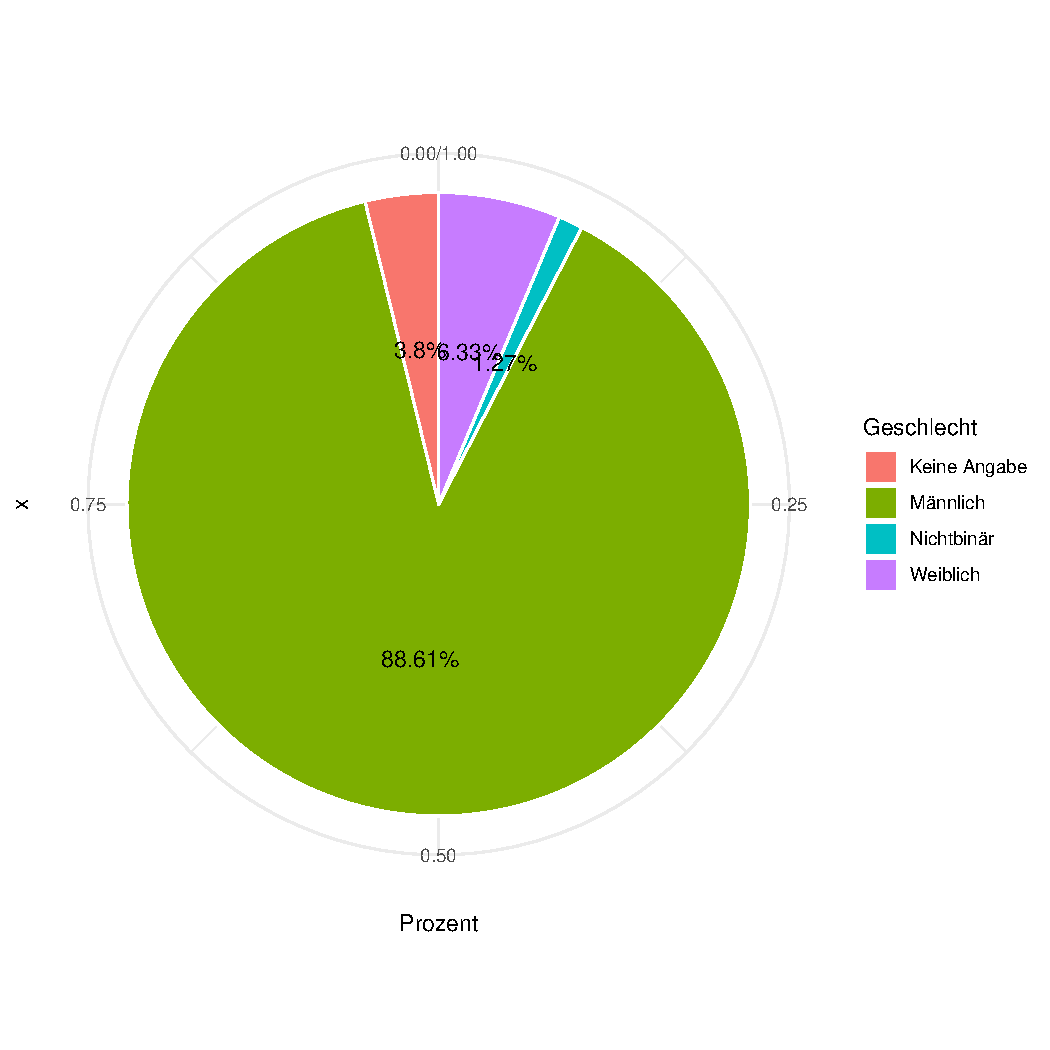
\includegraphics[width=0.7\columnwidth]{figures/plots/gender.pdf}
  \caption{\label{fig:piechart-gender} Geschlecht der befragten Personen}
\end{figure}

Das Kreisdiagramm in \autoref{fig:piechart-gender} zeigt, dass sich 88,61\% der befragten Personen mit dem männlichen Geschlecht identifizieren.
An dieser Stelle sei angemerkt, dass das Ergebnis der Auswertung mehrere Ursachen haben und die Ergebnisse bei Befragung einer anderen Personengruppe anders ausfallen kann.
Die ausgewählten Discord-Server enthalten überwiegend männliche Mitglieder, weswegen die Stichprobe voreingenommen sein kann.
Ebenso kann die Zielgruppe von Digimon oder Digimon World 1 bewusst primär das männliche Geschlecht sein.
Dies wird von der Aussage der interviewten weiblichen Person gestützt, dass diese sich nicht zugehörig zur Zielgruppe fühlt[P2, 658-660].\\

\begin{figure}[H]
  \centering
  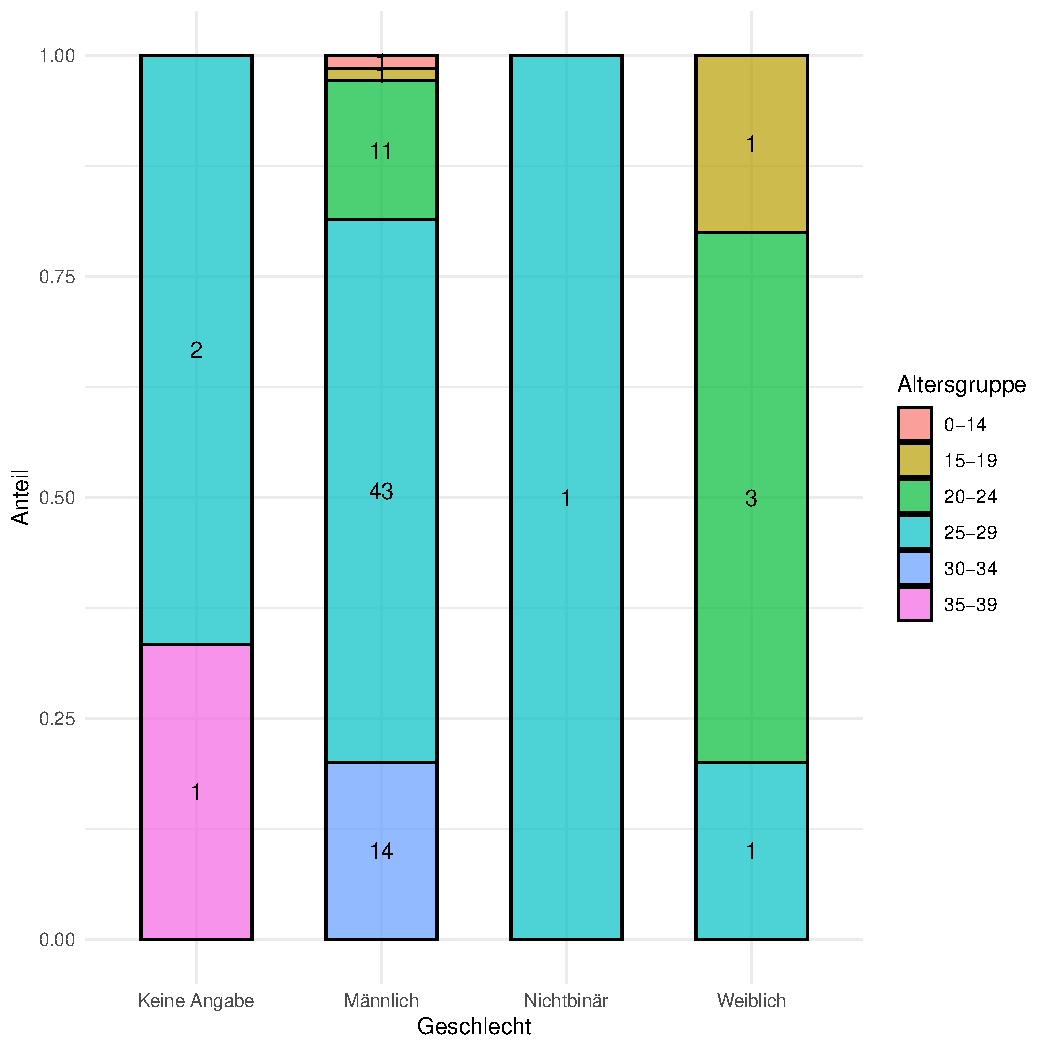
\includegraphics[width=0.65\columnwidth]{figures/plots/age_gender.pdf}
  \caption{\label{fig:age-gender} Altersgruppen innerhalb der Geschlechter}
\end{figure}

\autoref{fig:age-gender} zeigt die Verteilung der Altersgruppen innerhalb der Geschlechter.
Das Modell verdeutlicht, dass die Altersgruppe der Personen von 25-29 Jahren überwiegt.
Ebenfalls existieren keine befragten Personen in der Altersgruppe über 39 Jahren.
Es ist fraglich ob dies mit der Zielgruppe von Discord oder der tatsächlichen Zielgruppe von Digimon World zusammenhängt.
Lediglich eine einzige Person in der Altergruppe von 0-14 Jahren hat an der Umfrage teilgenommen.
Dies ist widersprüchlich, wenn die Klassenbreite\footnote{Die Klassenbreite $\Delta$ bezeichnet die Differenz der oberen und unteren Klassengrenze\cite[S.27]{elementare-stochastik}} von 14 betrachtet wird, da diese eine größere Gruppe von Personen eingrenzt als die anderen Altersklassen.
Allerdings kann die geringe Teilnahme dadurch erklärbar sein, dass die Discord-Nutzungsbedingungen nur Nutzer im Alter von mindestens 13 Jahren erlauben.
Aufgrund dieser Tatsache kann die tatsächliche Klassenbreite nur zwei betragen.
Bei den weiblichen Teilnehmern scheint die Altersgruppe im Vergleich zu den anderen Geschlechtern jünger zu sein.
Allerdings ist die Anzahl der befragten weiblichen Personen zu gering und es kann nur spekuliert werden, weswegen dies der Fall ist. \\

Im Januar 1999 bis Juli 2001 wurde Digimon World in unterschiedlichen Regionen veröffentlicht.
Innerhalb dieser Jahre wurde ebenfalls der Anime\footnote{In Japan produzierte Zeichentrickserie} Digimon Adventure in vielen Regionen veröffentlicht\cite{imdb-release}.
Digimon Adventure richtet sich primär an Kinder\cite{mal-adventure} und wurde unter anderem mit dem Begriff Shounen getaggt\cite{anidb-adventure}.
Der Begriff Shounen bezeichnet im japanischen die Zielgruppe von jungen männlichen Personen\cite{manga-brunner}.
Die starke Verteilung innerhalb der Altersgruppe von 25-29 Jahren kann erklärt werden, wenn diese zeitlich zum Zeitpunkt des Releases von Digimon World verlagert wird.
Wenn die Altersgruppe 25-29 um 20 Jahre zurückversetzt wird, beträgt die neu errechnete Altersgruppe 5-9 Jahre.
Aufgrund der Tatsache, dass die Altersgruppe mit der Zielgruppe von vor 20 Jahren übereinstimmt, ist davon auszugehen, dass viele Teilnehmer deswegen in diese Altersgruppe fallen, weil diese das Spiel vor 20 Jahren bereits gespielt haben.
Ebenfalls lässt sich der hohe männliche Anteil in der Verteilung durch diese Zielgruppe erklären. \\

\begin{figure}[H]
  \centering
  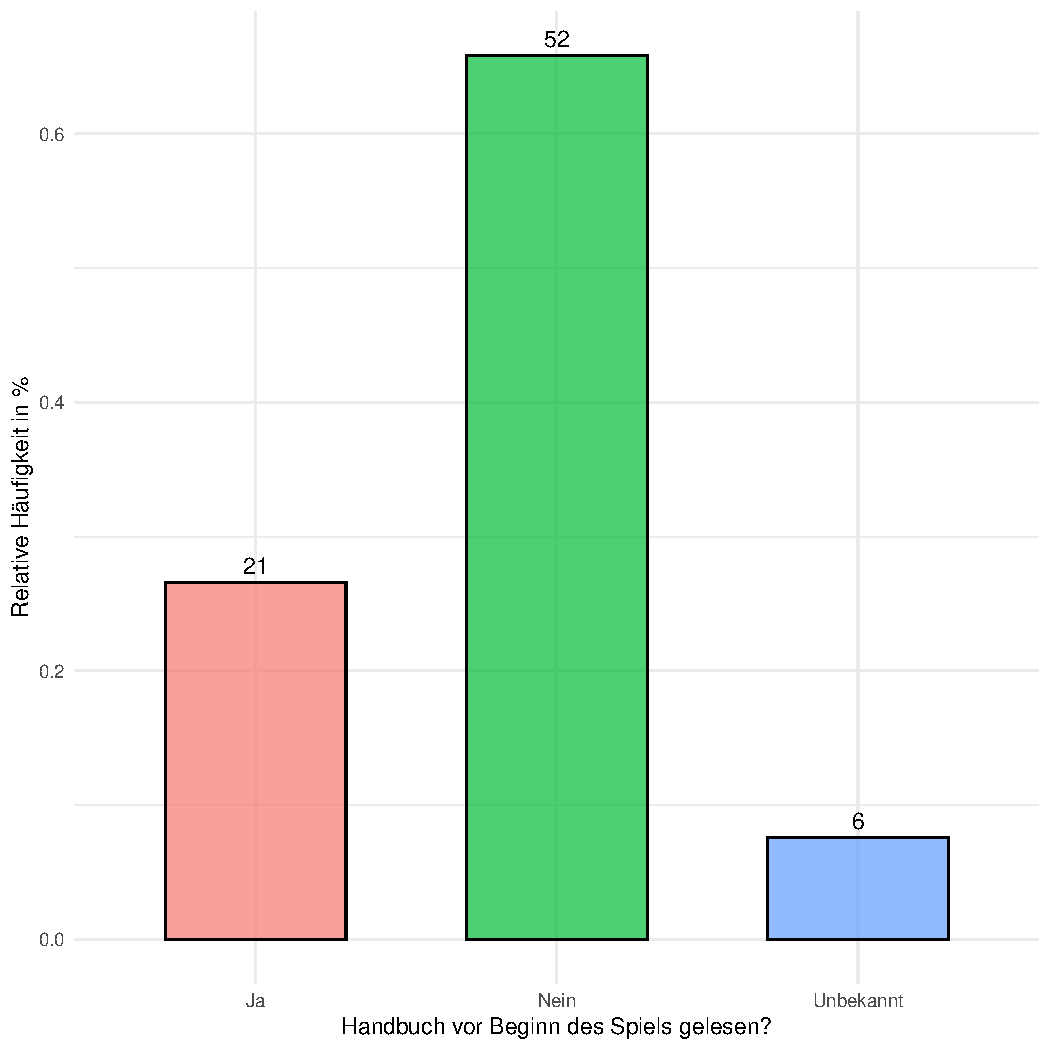
\includegraphics[width=0.65\columnwidth]{figures/plots/manual.pdf}
  \caption{\label{fig:manual} Anzahl der Personen, welche das Handbuch gelesen haben}
\end{figure}

Im Versuchsaufbau vom Interview in \autoref{sec:interview} ist aufgefallen, dass zwei Drittel (66,66\%) der interviewten Personen sich das Handbuch nicht angesehen haben.
Es wurde die Annahme gemacht, dass der Versuchsaufbau des Interviews irreführend sein könnte.
Das Säulendiagramm in \autoref{fig:manual} zeigt allerdings deutlich, dass 52 der 79 befragten Personen (65,8\%) ebenfalls das Handbuch vor Beginn des Spiels nicht gelesen haben.
Es spricht nichts dagegen, dass Personen im Verlauf des Spiels zum Handbuch greifen.
Allerdings verfehlt dies den Sinn und kritische Informationen könnten erst zu einem späteren Zeitpunkt für die Spielenden verfügbar sein.\\

\definecolor{LightGray}{gray}{0.9}
\begin{listing}[H]
  \caption{Analyse in R}
  \label{lst:correlation}
  \begin{minted}[
bgcolor=LightGray,
framesep=2mm,
baselinestretch=1.2,
fontsize=\footnotesize,
linenos,
]{r}
if (!require('pacman')) install.packages('pacman')
p_load(pacman, tidyverse, ggpubr, corrplot)

csv_df <- read.csv('data/results.csv')
df <- csv_df[, 14:30]

for (i in 1:17) {
  names(df)[i] <- sprintf('H%s', i)
}

correlations <- round(cor(df, method = 'spearman'), digits = 2)
corrplot(correlations, method = 'circle', type = 'upper')
correlations[abs(correlations) < 0.5 | correlations == 1] <- ''

for (i in 1:20) {
  df[, i] <- round(jitter(df[, i], factor = 0.3), digits = 3)
}

ggscatter(
  df,
  x = 'H11',
  y = 'H12',
  add = 'reg.line',
  conf.int = TRUE,
  cor.coef = TRUE,
  cor.method = 'spearman',
) +
  theme_minimal()
\end{minted}
\end{listing}

\autoref{lst:correlation} zeigt beispielhaft eine in der Arbeit ausgeführte Auswertung in R.
Zunächst werden benötigte Pakete mit dem Paketmanager pacman\cite{rdoc-pacman} geladen.
Anschließend werden die Daten in Zeile vier bis neun, aus der zuvor exportierten \ac{CSV}, geladen, in der Variable \texttt{df}\footnote{Üblich abgekürzter Variablenname für \texttt{data\_frame}} gespeichert und korrekt umbenannt.
Im Anschluss daran werden die Korrelationen zwischen den einzelnen Hypothesen nach Spearmans Korrelationskoeffizienten $\rho$ berechnet und auf zwei Nachkommastellen gerundet.
Spearmans Korrelationskoeffizient wird verwendet, um den Zusammenhang zwischen zwei rangskalierten Variablen zu bestimmten\cite{statistik-datenanalyse}.
Die berechnete Stärke des monotonen Zusammenhangs befindet sich im Intervall $[-1, 1]$, wobei $0$ kein Zusammenhang und $-1$ oder $1$ vollständiger monotoner Zusammenhang bedeutet.
An dieser Stelle sei angemerkt, dass Korrelation nicht gleich Kausalität bedeutet\cite[S.64]{elementare-stochastik}.
Es handelt sich zunächst lediglich um einen mathematischen Zusammenhang.
Diese Werte sind als symmetrische 17x17 Matrix in der Variable \texttt{correlations} gespeichert. \\

\begin{figure}[H]
  \centering
  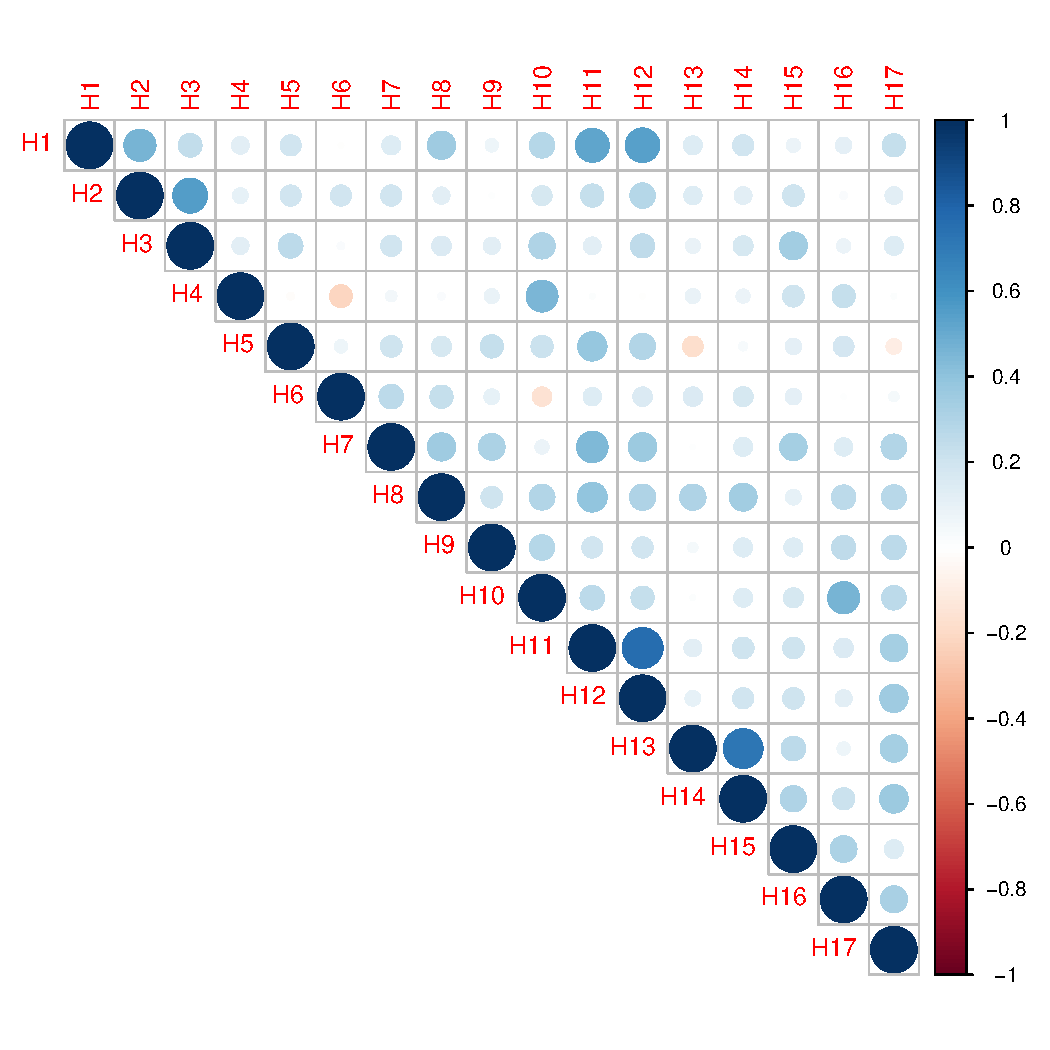
\includegraphics[width=0.65\columnwidth]{figures/plots/correlation.pdf}
  \caption{\label{fig:correlations} Korrelationsmatrix nach Spearmans $\rho$}
\end{figure}

Anschließend stellt Zeile zwölf im \autoref{lst:correlation} die Korrelationsmatrix, wie in \autoref{fig:correlations}, grafisch dar.
Aufgrund dessen, dass die Korrelationsmatrix symmetrisch ist, wird diese mithilfe der Option \texttt{type = upper} nur auf einer Seite der Hauptdiagonale erzeugt.
Das Ausblenden einer Seite dient der Übersicht.
Entlang der Hauptdiagonalen ist der Zusammenhang zwischen einer Hypothese mit sich selbst immer 1.
Jede Hypothese korreliert folglich perfekt mit sich selbst.
Diese Information bringt allerdings keinen Mehrwert.\\

Zeile 13 aus \autoref{lst:correlation} löscht die Werte der Hauptdiagonalen und aller Elemente, dessen absoluter Wert unter 0.5 fällt.
Diese Filterung wird durchgeführt, weil in dieser Arbeit nur die stärker korrelierenden Werte betrachtet werden\cite{cohen-power}.
Nach Ausführen der Funktion beinhaltet die symmetrische Matrix \texttt{correlations} nur noch zehn anstelle von 289 Einträgen.
Aufgrund der Symmetrie bedeutet dies, dass fünf Hypothesen einen Korrelationskoeffizienten von über 0.5 oder unter -0.5 betragen. \\

\begin{figure}[H]
  \centering
  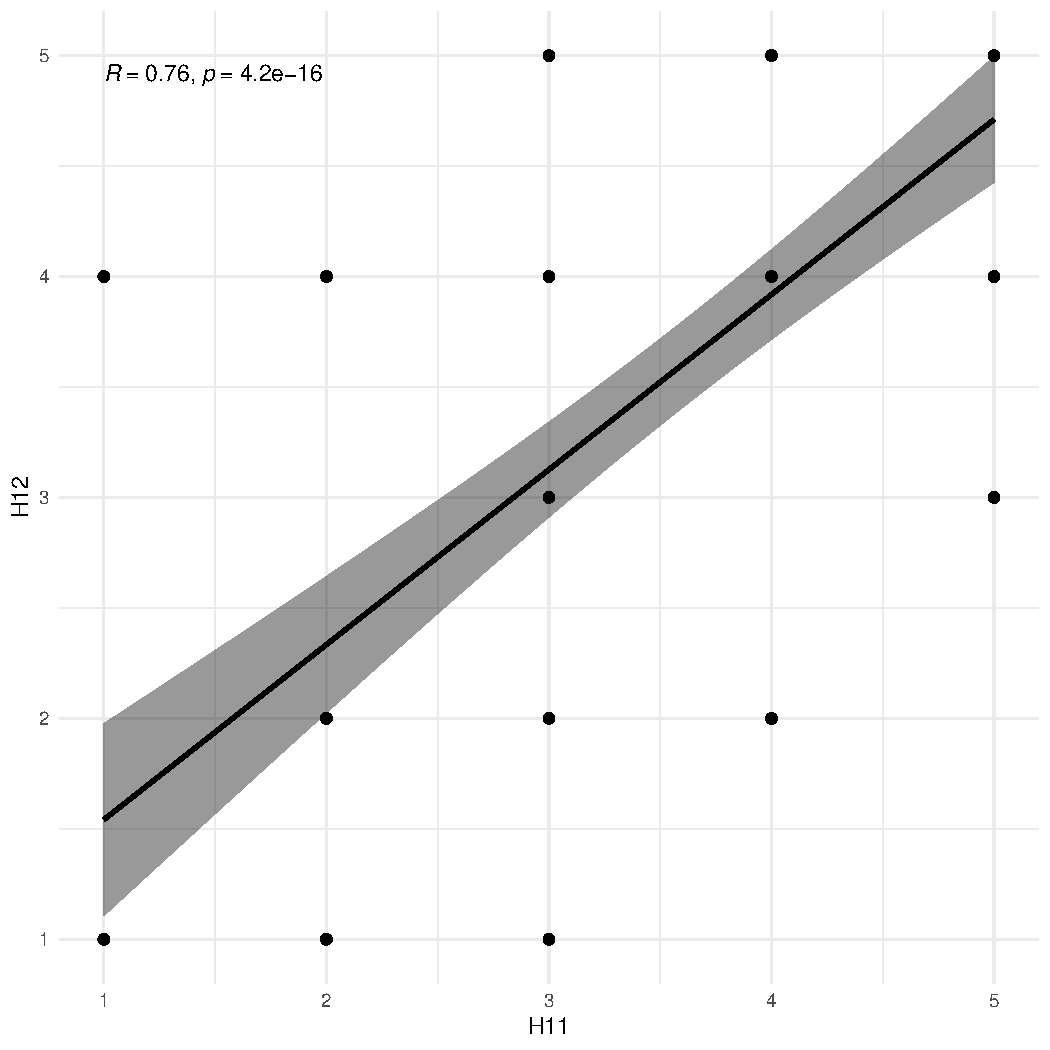
\includegraphics[width=0.65\columnwidth]{figures/plots/without_jitter.pdf}
  \caption{\label{fig:without_jitter} Streudiagramm - Korrelation zwischen H11 und H12}
\end{figure}

Mithilfe der Funktion \texttt{ggscatter} kann das Streudiagramm aus \autoref{fig:without_jitter} erstellt werden.
Diese Funktion wird in Zeile 19-28 in \autoref{lst:correlation} verwendet.
Das Diagramm stellt die Abhängigkeit der Hypothesen H11 und H12 dar.
Der errechnete Korrelationskoeffizient R nach Spearman beträgt 0,76.
Der p-Wert in \autoref{fig:without_jitter} misst die Wahrscheinlichkeit, dass ein Unterschied zwischen zwei, in der Arbeit ermittelten, Hypothesen zufällig sein könnte.
Wenn dieser Wert unter dem festgelegten Signifikanzniveau $\alpha$ von 0,05 liegt, ist das Ergebnis mit einer Fehlerwahrscheinlichkeit von p signifikant\cite[S.350]{elementare-stochastik}.
Dies ist hier der Fall, weswegen davon auszugehen ist, dass die Korrelation zwischen H11 und H12 nicht zufällig ist.
Die Fläche neben der Regressionsgeraden gibt die Wahrscheinlichkeit an, dass ein Wert mit 95\%-iger Wahrscheinlichkeit in diesen Bereich fällt.\\

Die Darstellung von \autoref{fig:without_jitter} ist allerdings irreführend, weil gleiche diskrete Werte sich überlagern und nicht unterschieden werden können.
Aus diesem Grund werden die Werte aus \texttt{df} mit der Funktion \texttt{jitter}\cite{jitter} zufällig, um einen kleinen Faktor, verändert.
Diese Funktion wird für alle Werte in \texttt{df} angewendet und befindet sich in Zeile 15-17 in \autoref{lst:correlation}.
Dies hat zur Folge, dass sich der R- und p-Wert ebenfalls verändern und das Resultat verfälscht wird.
Diese Herangehensweise wird hierbei nur verwendet, um die Daten anschaulicher darstellen zu können.

\begin{figure}[H]
  \centering
  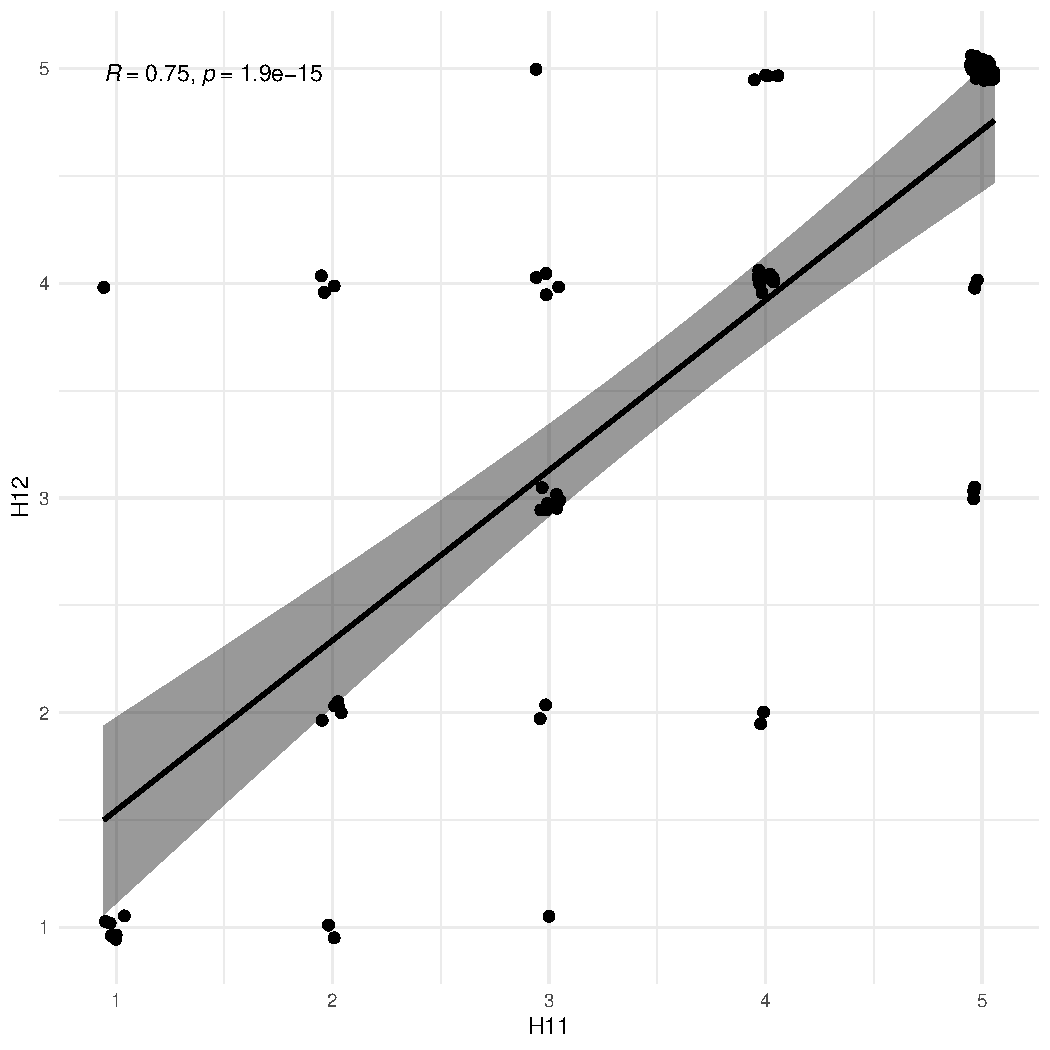
\includegraphics[width=0.65\columnwidth]{figures/plots/h11_h12.pdf}
  \caption{\label{fig:h11_h12} Verwackeltes Streudiagramm - Korrelation zwischen H11 und H12}
\end{figure}

Der positive Effekt dieser Herangehensweise lässt sich in \autoref{fig:h11_h12} erkennen.
Nach der Anwendung der Funktion \texttt{jitter} lassen sich gleiche Werte nun unterscheiden, weil diese sich nicht überlagern.
Die neu entstandenen Punktewolken verdeutlichen die Häufigkeiten der Antworten.
Alle weiteren, auf diese Art und Weise erzeugten, Graphen befinden sich im Anhang in \autoref{sec:scatterplots}.
Dort befindet sich auch die \autoref{table:correlations-overview}, welche die errechneten Werte ohne Anwendung der Funktion \texttt{jitter} zeigt.\\

Vier der fünf ermittelten Korrelationen deuten darauf hin, dass Personen, welche an zusätzlichen Informationen im Spiel interessiert sind, sich diese Informationen auch an anderen Stellen im Spiel wünschen.
Das bedeutet, dass davon auszugehen ist, dass eine Zielgruppe, welche sich allgemein mehr Informationen in Digimon World wünscht existiert.
Das gleiche Prinzip gilt bei der Korrelation zwischen neuem Aussehen des Charakters und der Auswahl des Geschlechts (siehe H13-H14 in \autoref{table:correlations-overview}).
Hier wird deutlich, dass Personen an der Personalisierung des Charakters im Allgemeinen interessiert sind.
Aus diesem Grund wird im Entwicklungsprozess darauf geachtet, dass korrelierende Funktionen gut aufeinander abgestimmt sind.\\

\begin{figure}[H]
  \centering
  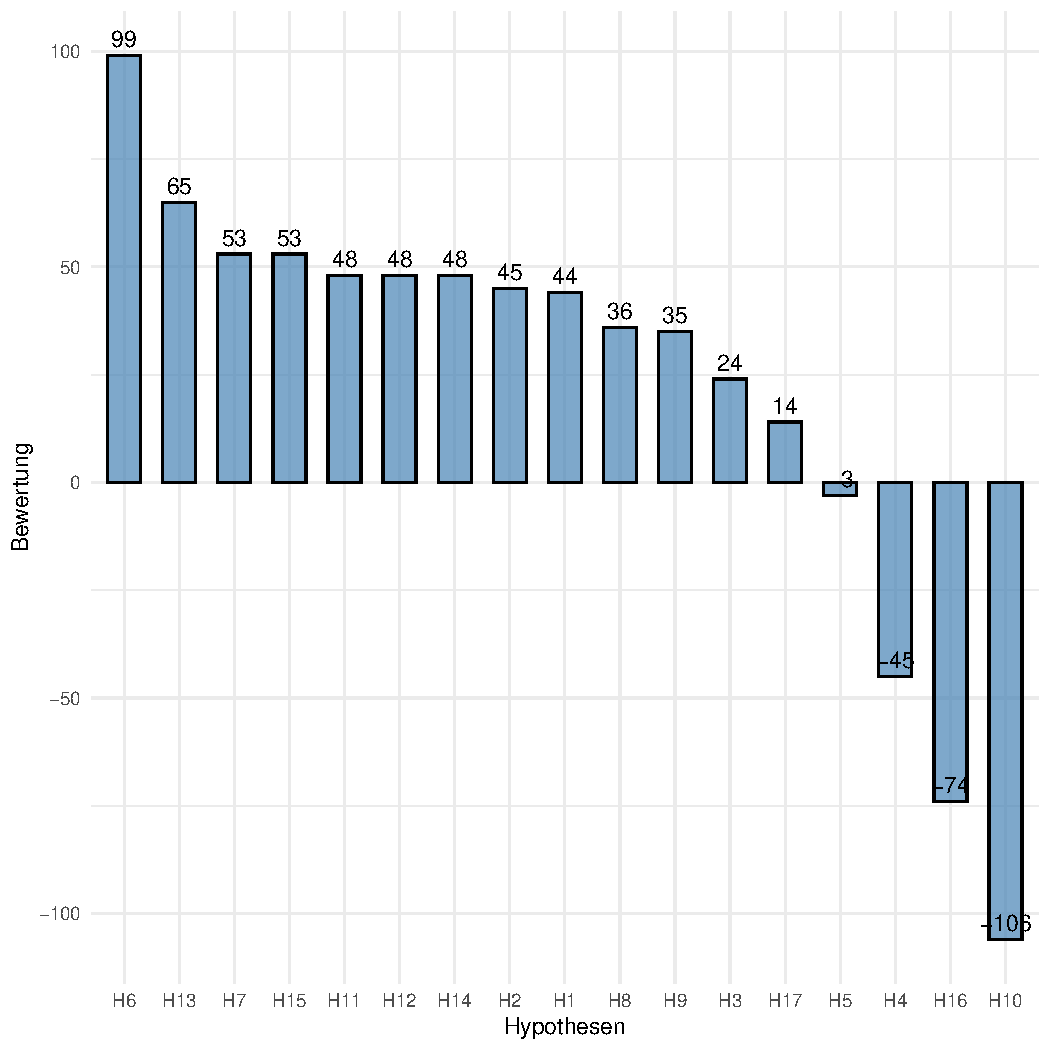
\includegraphics[width=0.8\columnwidth]{figures/plots/ranking.pdf}
  \caption{\label{fig:ranking} Einstufung der Hypothesen nach Priorität}
\end{figure}

Nachdem die vorliegenden Daten analysiert sind, werden diese in einem letzten Schritt nach Wichtigkeit sortiert.
Für dieses Verfahren ist die lineare Skala von 1 bis 5 auf $-2$ bis 2 abgebildet und ist pro Hypothese aufsummiert.
Dies hat den Vorteil, dass Features, welche nicht benötigt werden, auch deutlich in der \autoref{fig:ranking} erkennbar sind.
Die jeweilige Auswertung kann als Priorisierung für die einzelnen Aufgaben gesehen werden.

\subsection{User Persona}\label{sec:persona}
Als User Persona wird ein Modell bezeichnet, welches frei erfundene Nutzer repräsentiert\cite[S.123 f]{cooper-alan}. Dabei umfasst dieses Modell im Wesentlichen sowohl soziodemografische als auch psychografische Merkmale. Diese zeichnen sich durch Alter, Geschlecht, Familienstand, Motivation, Bedürfnisse und Persönlichkeit einer Person aus. Vorrangig werden dabei Merkmale verwendet, welche zur Identifizierung einer bestimmten Personengruppe relevant sind.
Das Ziel von Personas ist es, reales Nutzerverhalten zu simulieren und die Software an die Nutzenden anzupassen. Die neue, isolierte Zielgruppe ermöglicht es, Anforderungen gezielter gestalten zu können. Das liegt daran, dass User Personas konkrete fiktive Personen sind. Im Kontrast dazu steht der abstrakte Begriff eines Nutzers. Eine weitere wichtige Eigenschaft von Personas ist, dass diese stereotypisch gewählt werden. Dies verleiht den fiktiven Figuren mehr Glaubwürdigkeit\cite[S.127 f]{cooper-alan}. Damit der Bezug zur Entwicklung eines Videospiels nicht verloren geht, erhalten Personas ebenfalls technografische Merkmale\cite{tagungsband}. Diese Merkmale bilden die Einstellung und Präferenzen zu technischen Inhalten ab. \\

Die Zielgruppe ist in der durchgeführten Umfrage aus \autoref{sec:survey} stark heterogen ausgefallen. Im ersten Teil der Umfrage wird dies, anhand der demografischen Daten und Präferenzen, deutlich. Das Geschlecht der beteiligten Personen ist stark einseitig ausgefallen (siehe \autoref{fig:piechart-gender}). Allerdings soll das geplante Spiel alle sozialen Geschlechter ansprechen. Aus diesem Grund werden mehrere Personas entwickelt. Diese sind im Anhang in \autoref{fig:Persona1} und \autoref{fig:Persona2} dargestellt. Beide Personas gehören unterschiedlichen Altersgruppen und Geschlechtern an. Ebenso unterscheidet sich die Grundmotivation, Präferenzen und das technische Verständnis der entwickelten Personas. \\


\subsection{Szenario}
Klassischerweise wird an diesem Punkt der Ist-Analyse ein Ist-Szenario formuliert\cite[S. 419]{grundlagen-grochla}.
Dieses Szenario basiert auf dem Inhalt des Spiels Digimon World.
Die Hauptfigur des Szenarios ist die entwickelte Persona.
Bei mehreren Personas kann in Betracht gezogen werden, mehrere Szenarien zu verfassen.
Der Inhalt des Szenarios ist primär ein Ablauf innerhalb des Spiels.
Es soll bewusst problematische Situationen aufzeigen, welche einer Verbesserung bedürfen.
Typischerweise werden die Szenarios erneut in der Soll-Analyse als Soll-Szenario formuliert.
Allerdings werden Lösungsansätze präsentiert, welche die problematischen Situationen lösen.
Primär kann dadurch gezeigt werden, dass Abläufe optimiert oder Personas zufriedener mit der Gesamtsituation sind.
Auf das Ist-Szenario wird in dieser Arbeit verzichtet, weil Probleme bereits in den vorherigen Abschnitten deutlich beschrieben wurden.
Im folgenden \autoref{sec:wireframes} werden Lösungsansätze ebenfalls im Detail beschrieben und ein Bezug auf die entwickelten Personas genommen.
Aus diesem Grund wird das Soll-Szenario ebenfalls vernachlässigt.


\newpage
\section{Soll-Analyse}\label{sec:soll}
Die nachfolgenden Unterabschnitte verdeutlichen, wie der Entwicklungsprozess in \autoref{sec:entwicklungsprozess} stattfinden soll. Dabei sollen Vorgänge die, in den vorherigen Abschnitten ermittelten, Probleme lösen. Die Soll-Analyse vergleicht dann die geplante Umsetzung der Lösungen mit dem aktuellen Ist-Zustand aus \autoref{sec:ist}. Dadurch werden Ziele der Arbeit konkretisiert und Verbesserungen verdeutlicht.

\subsection{User Story}\label{sec:user-story}
Die Arbeit verwendet die Methode der User Stories\cite{scrum-user-stories}.
Üblicherweise wird eine User Story von einem Kunden auf einen A5 Zettel geschrieben.
Aufgrund dessen, dass kein konkreter Kunde für die Arbeit existiert, werden die Stories für die ermittelten Personas aus \autoref{sec:persona} verwendet.
Die Karten werden normalerweise nach einem bestimmten Muster geschrieben.
\glqq Als $<$Benutzerrolle$>$ will ich $<$das Ziel$>$[, so dass $<$Grund für Ziel$>$]\grqq{} ist hierbei ein typisches Muster.\\

Die User Stories funktionieren nach dem \ac{INVEST}-Prinzip\cite{user-stories}.
Das bedeutet, dass Stories untereinander keine Abhängigkeiten haben sollen.
Weiterhin sollen Karten verhandelbar sein.
Das bedeutet, dass die Funktionalitäten unter Umständen verändert werden können.
Diese Änderungen und Anmerkungen werden dann auf der Story-Karte notiert.
Die Story muss einen Wert für die Nutzenden besitzen und schätzbar sein.
Die zeitliche Einschätzung ist wichtig, weil ansonsten davon ausgegangen werden kann, dass das Domänenwissen fehlt oder die Story zu groß ist.
Ein Beispiel für dieses Verfahren wäre: \glqq Als Nutzerin will ich mich in der Spielwelt bewegen, sodass ich mit einem \ac{NPC} an einer anderen Position sprechen kann\grqq{}.\\

Allerdings ist ein Problem in diesem Verfahren, dass der Begriff des Nutzenden abstrakt ist.
Die in dieser Arbeit verwendete Vorgehensweise lehnt sich aus diesem Grund methodisch an die im Buch Story Driven Modeling\cite{story-driven-modeling} vorkommenden Beispiele an.
Der Vorteil ist, dass Story-Karten mit der Benennung der nutzenden Person konkreter werden.
Ebenfalls werden Stories durch die Beschreibung von Titel, Start-, Schritt- und Endsituation detaillierter.
Dies führt dazu, dass gleichzeitig die Testkriterien für die Story-Karten ermittelt werden.
Die Startsituation beschreibt den Anfangszustand und die Endsituation den Endzustand, welcher nach der durchgeführten Aktion vorhanden sein muss.
Üblicherweise eignen sich an dieser Stelle Tests, welche die Startsituationen mit einem Test überprüfen, eine Funktion aufrufen und die gewünschte Endsituation testen.\\

Die Tests von bestimmten Abschnitten und Funktionalitäten werden Unit-Tests genannt\cite{unit-tests}.
Sie werden in der Softwareentwicklung verwendet, um Fehler früher zu erkennen.
Ein weiterer Grund ist, dass Fehler, welche älteren Code unwirksam machen, früher entdeckt werden.
Die Entwicklung von Videospielen unterscheidet sich allerdings von anderen Bereichen der Software-Entwicklung\cite{difference-development}.
Das liegt daran, dass Spieletests menschenzentriert sind und menschliches Verhalten komplexer zu automatisieren ist\cite{testing-game-dev}.
Zusätzlich kann die Masse an möglichen Zuständen sehr groß sein.
Unit-Tests kommen in der Videospielentwicklung vor, allerdings wird ein stärkerer Fokus auf Usability-Testing gelegt\cite{no-unit-tests}.
Aus diesem Grund verzichtet diese Arbeit bewusst auf Unit-Tests.\\

Für die Durchführung der Methode werden Issues\cite{github-issues} anstelle von Story-Karten verwendet.
Diese digitale Variation der Story-Karten bietet mehrere Vorteile.
Ein Vorteil ist, dass Inhalte digital als Anhang integriert werden können.
Links zu externen Quellen sind per Mausklick abrufbar.
Weiterhin sind Inhalte nicht durch eine unleserliche Handschrift unbrauchbar.
GitHub bietet ebenfalls eine Funktion, Vorlagen für die Issues zu erstellen.
Dies vereinfacht den Prozess der Erstellung von Story-Karten zusätzlich.\\

Der größte Vorteil ist allerdings, dass GitHub automatisierte Kanban-Tafeln zur Verfügung stellt, in der Issues aufgelistet sind\cite{github-kanban}.
Kanban-Tafeln sind übersichtliche Darstellungen der Stories in einem Arbeitsablaufplan\cite{kanban-oreilly}.
Die in der Arbeit verwendete Tafel besitzt Spalten für Aufgaben, welche noch nicht begonnen wurden, aktuell in Bearbeitung oder fertig sind.
Der Grund für diese Methode ist die einhergehende Übersicht über den aktuellen Verlauf im Projekt.

\subsection{Entwurf}\label{sec:wireframes}
Ein weiterer Teil der Soll-Analyse ist die Erstellung von Wireframes.
Wireframes sind Design-Entwürfe für die grafische Benutzeroberfläche (\ac{GUI}).
Die Umsetzung erfolgt anhand von Papier-Prototypen\cite{prototyping-paper}.
Die einzelnen Design-Elemente sind als eigenes Stück Papier vorhanden.
Dies hat den Vorteil, dass einzelne Elemente schneller verschoben oder verworfen werden können.
Insbesondere wird bei der Entwicklung der Papier-Prototypen darauf geachtet, dass diese einen Bezug zu den Personas haben.
Die Papier-Prototypen werden anschließend digitalisiert in die Arbeit eingebunden.
Der Grund dafür ist, ähnlich wie bei den User Stories, um eine bessere Lesbarkeit zu gewährleisten.
Die nachfolgenden digitalen Prototypen sind nach Reihenfolge der in \autoref{sec:survey} ermittelten Priorität aufgelistet.\\

% lost items
\begin{figure}[H]
    \centering
    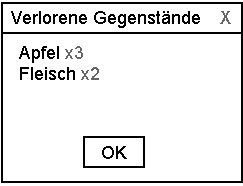
\includegraphics[width=0.4\columnwidth]{figures/wireframes/lost-items.pdf}
    \caption{\label{fig:lostitems}Verlorene Gegenstände}
\end{figure}

Die höchste positive Zustimmung hat die Hypothese erhalten, dass verlorene Gegenstände nach dem Verlust eines Lebens, der spielenden Person, angezeigt werden sollen.
Die Umsetzung dieser Funktionalität kann mithilfe eines zusätzlichen Pop-ups bewerkstelligt werden.
Der Inhalt in \autoref{fig:lostitems} zeigt alle Gegenstände an, welche verloren gegangen sind.
Ebenfalls wird die Menge angegeben.
Das Pop-up kann entweder mit dem OK-Knopf oder dem Kreuz verlassen werden. \\

Aufgrund der hohen Korrelation zwischen der Möglichkeit ein Geschlecht auszuwählen und dem Charakter Accessoires zu geben ist die Idee aufgekommen, dass ein Charakter-Editor sinnvoll wäre.
Dieser beinhaltet zunächst die Auswahl zwischen einigen Geschlechtern.
Dies erscheint allerdings nur bedingt sinnvoll, weil das Geschlecht im finalen Produkt keine Rolle spielen soll.
Ebenfalls ist keine eindeutige Zuordnung zwischen Aussehen und Geschlecht möglich, weil dieses divers ausfallen kann.
Spielende könnten über fehlerhafte oder mangelnde Pronomen verärgert werden\cite{rockpapershotgun-gender}. \\

\begin{figure}[H]
    \centering
    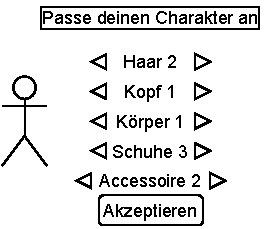
\includegraphics[width=0.5\columnwidth]{figures/wireframes/charselect.pdf}
    \caption{\label{fig:charselect}Charakter-Editor}
\end{figure}

Aus diesem Grund können Spielende über den Charakter-Editor den Charakter selber anpassen und personalisieren.
Ebenfalls sollen Spielende im Spiel nicht mit Pronomen angesprochen werden.
Diese Idee ist in \autoref{fig:charselect} zu sehen.
Die Auswahl an veränderbaren Eigenschaften beschränkt sich zunächst auf die abgebildeten Elemente.
Diese können mithilfe der Pfeile verändert werden.
Die Zahl hinter einem Element bildet die aktuelle Auswahl ab.
Diese kann dann mithilfe des Akzeptieren-Knopfes bestätigt werden. \\

Die Umfrage hat ergeben, dass Personen sich einen Indikator für vergangene Zeit nach einer Aktion wünschen.
Dies zeigt, dass für Spielende an mehreren Stellen nicht klar kommuniziert wurde, wie viel Zeit eine bestimmte Situation in Anspruch nimmt.
Deshalb kann dafür gesorgt werden, dass Hervorhebungen in Dialogen oder Animationen genaue Zeitangaben vermitteln.\\

Das Kampfsystem zu optimieren ist eine der schwierigsten zu bearbeitenden Hypothesen.
Das liegt daran, dass dies eine Kernmechanik ist und Änderungen dazu führen können, dass sich der Kerninhalt des Spiels ändert.
Die Änderung muss dabei zum Gesamtbild des Spiels passen.
Ebenso müssen die Wünsche der beiden Personas befriedigt werden.
Zum einen ist es wichtig, dass mehr Interaktionen möglich sind, zum anderen muss das Spiel auf passive Art und Weise spielbar sein.
Dies steht in einem starken Kontrast zueinander. \\

Aus diesem Grund ist die erste Idee, die Interaktionen nicht nur während des Kampfes, sondern auch vor dem Kampf zu erhöhen.
Sobald ein Kampf stattfindet, soll die spielende Person zunächst eine Phase der Vorbereitung durchlaufen.
Dort können Aktionskarten zu einem Kartendeck zusammengestellt werden.
Die auswählbaren Karten sind abhängig vom Typ des Digimons.
Ebenfalls wird die Mechanik verworfen, Gegenstände im Kampf zu verwenden.
Diese Mechanik wird durch die neuen Aktionskarten ersetzt.
Im Kampf bestimmt die aktuelle Menge von Magie, welche Karte ausgespielt werden kann.
Die Idee ist, dass Karten Angriffe oder Effekte erzwingen können, welche der Partner sonst nur zufällig auswählen kann.
Die Angriffe haben dann jeweils abhängig der Intelligenz des Partners eine prozentuale Chance den Gegner zu treffen.
Schwächere Angriffe haben eine hohe und stärkere Angriffe eine niedrige Chance zu treffen.
Dadurch entsteht eine Relation zwischen Belohnung und Risiko.
Dies soll den spielenden taktische Entscheidungen ermöglichen. \\

Digimon World besitzt das Problem, dass an einigen Stellen im Kampf ein Stunlock vorkommen kann.
Das bedeutet, dass ein Gegner permanent angegriffen wird, ohne reagieren zu können.
Dies passiert primär bei zu hoher Geschwindigkeit, weil der Gegner seinen Angriff immer langsamer ausführt als das eigene Digimon.
Um dieses Problem zu beseitigen, sollen Digimon Angriffe nacheinander ausführen.
Dies gleicht einer rundenbasierten Kampfmechanik. \\

Dieses System wurde mehrfach überarbeitet, weil es viele Probleme beinhaltet.
Das erste Problem ist, dass die klare Trennung zwischen Digimion und der spielenden Person verloren geht.
In dieser Kampfmechanik agiert nur die spielende Person.
Gleichermaßen wird die Persona Elena keine Möglichkeit haben, das Spiel zur Entspannung zu verwenden, weil das Kartensystem eine zu hohe Komplexität besitzt. \\

\begin{figure}[H]
    \centering
    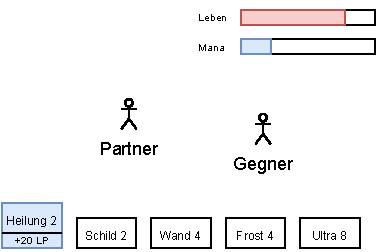
\includegraphics[width=0.8\columnwidth]{figures/wireframes/battle.pdf}
    \caption{\label{fig:battle-wireframe}Kampfsituation}
\end{figure}

Nach mehreren Iterationen der Optimierung ist das gewünschte Ergebnis erreicht.
Dieses ist in \autoref{fig:battle-wireframe} dargestellt.
Für die Erklärung wird anfänglich das Kampfsystem von Digimon World als Basis genommen.
Zunächst wird die maximale Menge an verfügbaren Magiepunkten auf zehn reduziert.
Diese war zuvor variabel. Ebenfalls startet jeder Kampf mit drei Magiepunkten.
Die Idee, Karten im Kampf verwenden zu können, wird zunächst von der vorherigen Iteration übernommen.
Allerdings erzwingen diese keine Angriffe, sondern wirken unterstützende Effekte.
Dadurch kann der Partner alleine agieren und die spielende Person wirkt als Unterstützer.
Dies hat zur Folge, dass weiterhin eine klare Trennung zwischen beiden Charakteren existiert.
Die verfügbaren Aktionskarten unterscheiden sich pro Partner und können vom Typ abhängig sein.
Jeder Partner besitzt fünf verfügbare Aktionskarten.
Die Kosten für diese belaufen sich auf zwei, zwei, vier, vier und acht Magiepunkte.
Je mehr eine Aktionskarte kostet, desto wirkungsvoller ist diese.
Durch jene Verteilung entstehen zwei Vorteile.
Zum einen die Relation zwischen Belohnung und Risko, zum anderen verschiedene Optionen für die taktischen Entscheidungen.
Die Karte für acht Magiepunkte ist sehr mächtig, allerdings muss abgewogen werden, ob der Partner nicht früher auf andere Aktionskarten angewiesen ist.\\

Im Kampf sollen im Vorfeld bereits mehr der in Digimon World vorkommenden Optionen verfügbar sein.
Das bedeutet, dass die Optionen aggressiver, defensiver oder scheuer Spielstil bereits zu Beginn verfügbar sind.
Dadurch wird der Parameter Intelligenz vom Kampf entkoppelt.
Diese Optionen sind nicht in \autoref{fig:battle-wireframe} modelliert.
Das liegt daran, dass die Verhaltensweisen in einem weiteren Schritt in der Zukunft zunächst näher untersucht werden müssen.
Das Spiel rundenbasiert zu entwerfen widersetzt sich der Natur des Spiels.
Aus diesem Grund soll der Stunlock durch einen Rückstoß ersetzt werden.
Ebenfalls wird bei jedem Angriff beiden Gegnern Schaden zugefügt.
Magiepunkte können aufgeladen werden, wenn die spielende Person kurz vor einem Angriff eine entsprechende Taste betätigt.
Falls eine Person kein Interesse an dieser Funktionalität hat, kann dies in den Spieleinstellungen deaktiviert werden.
Aus Sicht von Christian ensteht durch diese neue Kampfmechanik mehr taktisches Vorgehen und mehr Interaktion.
Elena hingegen besitzt weiterhin die Option, dem Partner beim Kämpfen zuzusehen und einen simpleren Spielstil zu wählen.\\

\begin{figure}[H]%
    \centering
    \subfloat[\centering Final Fantasy XIV]{{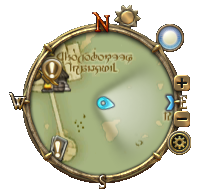
\includegraphics[width=4cm]{figures/screenshots/ff14.png}
                \label{fig:ff14}}}%
    \qquad
    \subfloat[\centering Wireframe]{{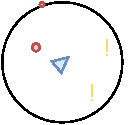
\includegraphics[width=4cm]{figures/wireframes/minimap.pdf} }\label{fig:minimap-wireframe}}%
    \caption{Minimap in Anlehnung an Final Fantasy XIV}%
    \label{fig:minimap}%
\end{figure}

Eine der gänzlich neu hinzugefügten Funktionalitäten ist die Minimap\footnote{Miniaturkarte}.
Diese wurde sich vermehrt von den befragten Personen gewünscht, weil die Spielwelt alleine nicht übersichtlich genug ist.
Aus der Analyse ist hervorgegangen, dass die Existenz und zusätzliche Informationen auf der Minimap mit einer Aufgabenliste korreliert.
Die Aufgabenliste wird später in diesem Abschnitt erwähnt.
Eine mögliche Interpretation dieser Korrelation ist in \autoref{fig:minimap} zu sehen.
Dabei lehnt sich die entwickelte Minimap an die im Spiel Final Fantasy XIV vorkommende Minimap an.
Im Wireframe markieren gelbe Ausrufezeichen offene Aufgaben und rote Punkte Gegner.
Wenn ein Symbol aus dem sichtbaren Bereich der Minimap verschwindet, wird dieses Symbol verkleinert am Rande der Minimap dargestellt.
Das sorgt dafür, dass die spielende Person die ungefähre Position eines Ziels ermitteln kann.
Die spielende Person wird durch ein blaues Symbol dargestellt.
Die Position ist innerhalb der Minimap immer zentriert und die Ausrichtung gibt die aktuelle Rotation in der Spielwelt an.

\begin{figure}[H]
    \centering
    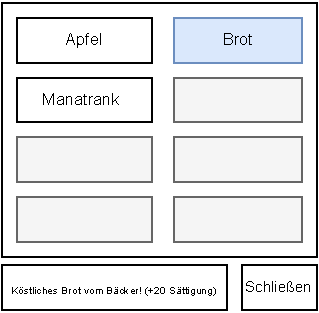
\includegraphics[width=0.5\columnwidth]{figures/wireframes/inventory.pdf}
    \caption{\label{fig:inventory}Inventar}
\end{figure}

Zusätzliche Informationen im Inventar korrelieren mit zusätzlichen Fortschrittsbalken für Sättigung und Toilettenbedarf.
Die vorgenommene Änderung beläuft sich nur auf Textinhalte im Inventar.
\autoref{fig:inventory} zeigt beispielhaft den ausgewählten Gegenstand Brot.
Die Beschreibung gibt an, welche Attribute des Partners sich bei einer Verwendung des Gegenstands verändern.
Bezüglich des Inventars wurde eine weitere Entscheidung getroffen.
In Digimon World wird das Inventar für viele Zwecke verwendet.
Dementsprechend erhöht sich die Häufigkeit, wie oft die spielende Person dieses Menü betrachtet.
Wenn ein Digimon Hunger hat, muss es mit Nahrungsmitteln gefüttert werden.
Manchmal kommt es vor, dass eine Nahrungsration nicht ausreicht.
Das Problem ist allerdings, dass sich das Inventar nach jeder Anwendung einer Nahrungsration schließt.
Dieses Problem soll künftig vermieden werden.
Ebenfalls existiert für das Inventar kein Zwischenmenü.
Dies verringert die Benutzungstiefe.
Das Inventar wird im neuen Spiel dann standardmäßig mit der Taste \texttt{I}, für Inventar oder Inventory, geöffnet.
Das Inventar besitzt begrenzte Plätze und es ist zunächst nicht geplant, dass diese erweitert werden können.
Die Begrenzung soll dafür sorgen, dass Spielende sich bewusst dazu entscheiden, welche Vorräte sie bei der Erkundung benötigen.\\

\begin{figure}[H]
    \centering
    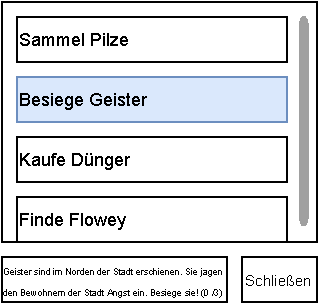
\includegraphics[width=0.5\columnwidth]{figures/wireframes/journal.pdf}
    \caption{\label{fig:journal}Aufgabenliste}
\end{figure}

\autoref{fig:journal} zeigt ein Wireframe für die Aufgabenliste.
Die Aufgabenliste ist ähnlich zum Inventar aufgebaut.
Jedoch ist die Anzahl der annehmbaren Aufgaben nicht begrenzt.
Die Spielenden sollen frei entscheiden, welchen Aufgaben sie sich zuerst widmen.
Bei der Auswahl einer Quest wird diese farblich hervorgehoben und eine Beschreibung erklärt detailliert, was getan werden muss, um die Aufgabe zu erfüllen.
Ebenfalls ist es wie beim Inventar möglich, das Journal mit einer Taste zu öffnen.
Die hierfür gewählte Taste ist \texttt{J}.
Diese Taste ist ebenfalls eine typische Abkürzung in Videospielen und steht für Journal.
Geschlossen werden können beide Menüs mithilfe des Schließen-Knopfes, der Betätigung der entsprechenden Taste (\texttt{I}/\texttt{J}) oder der \texttt{ESC}-Taste.\\

Eine andere Funktionalität, welche sich oft gewünscht wurde, sind weitere visuelle Hinweise, wie beispielweise Knöpfe im \ac{HUD}.
Diese sollen angezeigt werden, wenn der Videospielcharakter mit einem Objekt oder einem \ac{NPC} interagieren kann.
Die Idee ist in diesem Fall, dass der entsprechende Knopf über dem Objekt erscheint, wenn sich der Spieler im entsprechendem Radius befindet.\\

\begin{figure}[H]%
    \centering
    \subfloat[\centering Uhr in Digimon World]{{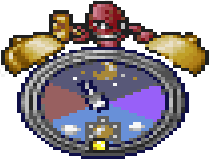
\includegraphics[width=4cm]{figures/screenshots/clock.png}
                \label{fig:clock}}}%
    \qquad
    \subfloat[\centering Fortschrittsbalken]{{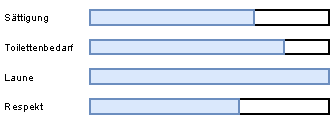
\includegraphics[width=7cm]{figures/wireframes/progressbars.pdf} }\label{fig:progressbars}}%
    \caption{Uhr und Fortschrittsbalken}%
    \label{fig:clock-progress}%
\end{figure}

Die Uhr in Digimon World, welche in \autoref{fig:clock} dargestellt ist, konnte zunächst von den interviewten Personen nicht korrekt gedeutet werden.
Dies brachte die Hypothese auf, dass diese durch eine Uhr mit zwei Zeigern ersetzt werden sollte.
Die Mehrheit der Personen in der Umfrage stimmten dieser Aussage zu.
Das bedeutet, dass in der Implementierung eine Uhr mit zwei Zeigern nötig ist. \\

Aufgrund einer ungünstigen Formulierung in der Umfrage stellte sich heraus, dass Personen kein Interesse daran haben, einen Fortschrittsbalken, welcher zwei Mal voll werden muss, in einen Fortschrittsbalken zu ändern, welcher nur einmalig gefüllt werden muss bis der Maximalwert erreicht ist.
Teilnehmende Personen der Umfrage haben die Aussage, Glück und Disziplin nicht zu spalten, so verstanden, dass Glück und Disziplin ein neuer Wert Glück-Disziplin ist.
Nach einer weiteren Nachfrage stellte sich heraus, dass einige teilnehmende Personen ansonsten zugestimmt hätten.
Aus diesem Grund werden die Fortschrittsbalken so angepasst, dass diese nur ein Mal voll werden können.
Ebenfalls werden weitere Informationen wie Sättigung und Toilettenbedarf hinzugefügt.
Diese sind in \autoref{fig:progressbars} zu sehen.
Zusätzlich werden keine Symbole verwendet, sondern Texte, welche den Inhalt der Fortschrittsbalken beschreiben.
Dies soll Missverständnisse vermeiden.\\

Die Hyptothese, ein Tutorial hinzuzufügen, wird in dieser Arbeit zunächst vernachlässigt.
Das liegt daran, dass diese eine niedrige Bewertung im Ranking besitzt.
Viel wichtiger ist jedoch die Tatsache, dass für die Implementierung zunächst das Kampfsystem und technische Funktionalitäten im Fokus stehen.
Die Erkenntnis, dass das Tutorial im Spiel vorhanden sein muss und damit einen Einstieg im Spiel bietet, ist jedoch deutlich.
Das Tutorial ist nach Implementierung der Kernfunktionalitäten in Form einer spielerischen Anleitung geplant.
Das bedeutet, dass Spieler mithilfe von Aufgaben Menüs, Kampfmechaniken oder die vorhin genannten Funktionalitäten erkunden können.
Texttutorials wurden in Erwägung gezogen, allerdings widersprechen diese dem Persona von Christian.
Dieser möchte Spielinhalte durch Handeln erlernen und keine langen Erklärungstexte lesen.


\newpage
\section{Entwicklungsprozess}\label{sec:entwicklungsprozess}
Die in den folgenden Abschnitten vorkommenden Methoden stützen sich auf die in der Arbeit erarbeiteten Daten. Dabei werden die ermittelten Hypothesen aus \autoref{sec:survey} verwendet. Die Priorität legt dabei den Verlauf des Entwicklungsprozesses fest. Der Entwicklungsprozess richtet sich nach den in \autoref{sec:user-story} vorgestellten User Stories und den in \autoref{sec:wireframes} entwickelten Wireframes. Dabei wird die Zielgruppe der in \autoref{sec:persona} erwähnten Personas nicht vernachlässigt. Die nachfolgenden Abschnitte beschreiben die Entwicklung der Anwendung. Ebenfalls werden zwei unterschiedliche Methoden beschrieben, welche die Entwicklung validieren.

\subsection{Spiel-Engine}
Eine Spiel-Engine für die Entwicklung von Videospielen zu verwenden ist heutzutage üblich.
Spiel-Engines lassen sich in diverse modulare Bestandteile zerlegen.
So besteht eine Spiel-Engine oftmals aus Physik-, Grafik- und Audiomodulen.
Je nach Spiel-Engine können diese Module auch variieren.
Für die Ausarbeitung des Projekts wird die neueste Version der Godot Engine (v.3.4) verwendet\cite{godot-website}.
Um die Auswahl näher erläutern zu können, wird die Godot Engine in der folgenden \autoref{table:game-engine-overview} zwei populären Spiel-Engines gegenübergestellt. \\

\begin{center}
  \begin{table}[!ht]
    \centering
    \begin{tabular}{ l | c | c | c }
                             & Godot Engine                & Unity    & Unreal Engine \\
      \hline
      \hline
      Programmiersprachen    & GDScript, C\texttt{++}, C\# & C\#      & C\texttt{++}  \\
      Lizenz                 & MIT                         & EULA     & EULA          \\
      Source-Code zugänglich & \cmark                      & \xmark   & \cmark        \\
      Itch.io-Anteil         & $2,5\%$                     & $47,3\%$ & $2,8\%$       \\
      Steam-Anteil           & -                           & $13,2\%$ & $25,6\%$      \\
      Veröffentlichungsjahr  & 2014                        & 2005     & 1998          \\
    \end{tabular}
    \caption{Spiel-Engines im Vergleich}
    \label{table:game-engine-overview}
  \end{table}
\end{center}

Die Godot Engine unterstützt aktuell drei verschiedene Programmiersprachen, welche in \autoref{table:game-engine-overview} aufgelistet sind.
GDScript ist eine für die Godot Engine entwickelte Programmiersprache, welche der Pythonsyntax stark ähnelt\cite{godot-dynamic-lang}.
GDScript ist dynamisch typisiert und verfolgt ebenfalls Konzepte des Duck-Typings\cite{duck-typing}.
Jedoch ist es möglich, in GDScript eine statische Typisierung zu verwenden.
Eine statische Typisierung ermöglicht die automatische Vervollständigung für alle Methoden und Variablen eines Typs.
Dies ist nicht nur vorteilhaft für die Entwicklung, sondern erhöht auch die Geschwindigkeit der Anwendung\cite{godot-static}.
Das liegt daran, dass Typen nicht während der Laufzeit ermittelt werden müssen.
Aus diesem Grund gibt es weniger Rechenoperationen.
Mithilfe der dynamischen Typisierung ist dies nicht möglich, weil der Typ einer Variable erst zur Laufzeit bekannt ist. \\

Die Godot Engine und Unreal Engine unterstützen die Programmiersprache C\texttt{++}.
C\texttt{++} ermöglicht eine genaue Kontrolle des Speichermanagements.
Dies kann allerdings nachteilig sein, weil die Garbage Collection\footnote{Automatische Bereinigung des Speichers} nicht vorhanden ist und der Speicher manuell bereinigt werden muss.
Unreal Engine versucht diesem Problem mithilfe einer eigenen Garbage Collection für Objekte vom Typ \texttt{UObject} entgegenzuwirken\cite{unreal-garbage}.
Ebenfalls verfügt Unreal Engine über ein eigenes Property System, welches Reflection ermöglicht\cite{unreal-reflection}.
Die Godot Engine besitzt diese Features allerdings nicht.
Trotzdessen ist C\texttt{++} aufgrund der genauen Kontrolle über Speicherzuweisungen und der Optimierungsmöglichkeiten relevant.
Im Vergleich zur Unreal Engine ist es allerdings auch möglich, auf diese Features zu verzichten, wenn eine Optimierung von vornherein nicht notwendig ist.
Optimierungen kosten Arbeitszeit und sind nicht immer notwendig.\\

Die letzte, in \autoref{table:game-engine-overview} vorkommende, Programmiersprache ist C\#.
Diese wird von Unity und der Godot Engine unterstützt.
C\# ist eine statische Programmiersprache, welche den Speicher mithilfe eines Garbage Collectors selbst verwaltet.\\

Ein weiterer Unterschied zwischen den Spiel-Engines sind die unterschiedlichen Lizenzen und die Einsicht vom Editorcode.
Unity und Unreal Engine fallen unter eine Endbenutzer-Lizenzvereinbarung.
Diese besagt, dass beide Spiel-Engines unter dem Rahmen einer proprietären Software fallen und je nach Umsatz des Spieltitels Gebühren anfallen können\cite{unity-price}\cite{unreal-price}.
Unity besitzt, als einzige der drei vorgestellten Spiel-Engines, keinen frei zugänglichen Quelltext.
Das bedeutet, dass Fehler innerhalb der Spiel-Engine, welche während der Produktion des Spiels auffallen, nicht selbst behoben werden können.
In diesem Fall muss darauf gehofft werden, dass das Unity-Entwicklerteam sich dazu entscheidet, diesen Fehler zu beheben.
Dies kann jedoch viel Zeit in Anspruch nehmen. Der Quellcode von Unreal Engine ist erst nach Akzeptierung eines Endbenutzer-Lizenzvertrags einsehbar.
Die Godot Engine besitzt im Vergleich zu Unity und Unreal Engine keine Einschränkungen bei der Einsicht des Quellcodes.
Ebenfalls fallen aufgrund der MIT-Lizenz keine Kosten an. \\

\autoref{table:game-engine-overview} enthält ebenfalls Informationen über die beiden Verkaufsplattformen Steam und Itch.io\cite{steam-website}\cite{itchio-website}.
Itch.io richtet sich primär an die Entwicklung und den Verkauf von Indie-Spielen.
Indie-Spiele werden üblicherweise von kleinen Entwicklerteams entwickelt.
Im Kontrast dazu stehen große Entwicklerstudios wie Ubisoft, Riot Games oder das Entwicklerstudio Valve Corporation, welches Steam und zahlreiche Spiele entwickelt hat\cite{ubisoft-website}\cite{riotgames-website}\cite{valve-website}.
Die Daten für Steam und Itch.io sind einer Studie entnommen, welche den Markt im Dezember 2018 untersucht hat\cite{taxonomy}.
Im Rahmen dieser Arbeit wurden diese Daten mit einem aktuelleren Stand verglichen.\\

\begin{center}
  \begin{table}[!ht]
    \centering
    \begin{tabular}{ l | c | c | c}
      Spiel-Engine   & \%-Anteil 2018 & \%-Anteil 2021 & Anstieg \\
      \hline \hline
      Unity          & $47,3\%$       & $52,34\%$      & \cmark  \\
      Construct      & $12,3\%$       & $11,29\%$      & \xmark  \\
      GameMaker      & $11,0\%$       & $7,64\%$       & \xmark  \\
      Twine          & $6,2\%$        & $4,87\%$       & \xmark  \\
      RPG Maker      & $3,9\%$        & $2,85\%$       & \xmark  \\
      Bitsy          & $3,3\%$        & $2,99\%$       & \xmark  \\
      PICO-8         & $2,9\%$        & $2,66\%$       & \xmark  \\
      Unreal         & $2,8\%$        & $2,99\%$       & \cmark  \\
      Godot          & $2,5\%$        & $5,21\%$       & \cmark  \\
      Ren'Py         & $2,0\%$        & $1,88\%$       & \xmark  \\
      Andere Engines & $5,9\%$        & $5,29\%$       & \xmark  \\
    \end{tabular}
    \caption{Trends auf Itch.io im Vergleich}
    \label{table:game-engine-percent}
  \end{table}
\end{center}

Die konkreten Daten, für die vorgenommene Auswertung, befinden sich im Anhang der Arbeit in einer \ac{CSV}-Datei und sind der Website von Itch.io entnommen\cite{most-projects}.
\autoref{table:game-engine-percent} zeigt deutlich, dass die in der Arbeit vorgestellten Spiel-Engines einen prozentualen Anstieg der Popularität in den letzten drei Jahren erfahren haben.
Alle weiteren Spiel-Engines sanken in der Popularität.
Die Spiel-Engine Unity bleibt weiterhin auf dem ersten Platz und umfasst nun mehr als die Hälfte aller entwickelten Projekte auf Itch.io.
Der Unterschied zwischen der Unreal Engine und der Godot Engine betrug im Jahr 2018 $0{,}3\%$.
Die Godot Engine hat ihre Popularität in den letzten drei Jahren allerdings mehr als verdoppelt.
Dadurch ist die Godot Engine im Indie-Bereich nun populärer als die Unreal Engine.
Der Unterschied zwischen den beiden Engines beträgt nun $2{,}22\%$.
Zusätzlich befindet sich die Godot Engine nun in den Top vier der meist genutzten Spiel-Engines auf Itch.io.
Das bedeutet, dass die Godot Engine immer relevanter für die Entwicklung in kleinen Entwicklerteams geworden ist.
Aufgrund dieser Punkte ist die Arbeit mit der Godot Engine ausgearbeitet. \\

\subsection{Entwurfsmuster}
Entwurfsmuster sind ein fester Bestandteil der Godot Engine.
Einige dieser Entwurfsmuster werden in der Arbeit verwendet.
Die bereits existierenden Entwurfsmuster werden zusätzlich um zwei weitere Entwurfsmuster erweitert.
Diese werden im Folgenden erläutert, allerdings wird zunächst die Grundarchitektur näher erklärt.
Komponenten oder Objekte der Architektur werden als Nodes bezeichnet.
Diese Nodes sind Teil eines Baumgraphen.
Der Wurzelknoten dieses Baumgraphen wird als Szene oder Szenengraph bezeichnet.\\

\begin{figure}[ht]
	\centering
	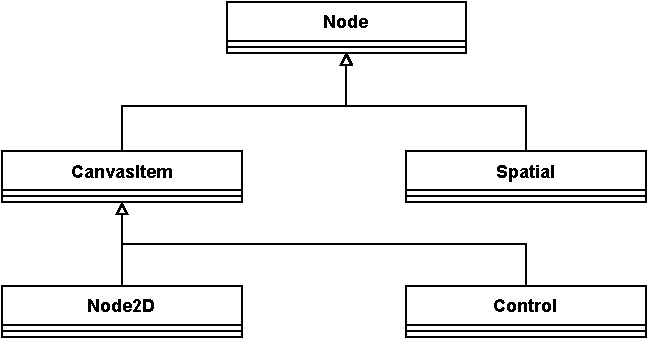
\includegraphics[width=0.8\columnwidth]{figures/node-graph.pdf}
	\caption{\label{fig:nodegraph} Node-System}
\end{figure}

\autoref{fig:nodegraph} veranschaulicht einen Ausschnitt aus dem Architekturdiagramm der Godot Engine\cite{godot-architecture}.
Spatial sind Nodes, welche eine Node im dreidimensionalen Raum abbilden.
Das bedeutet, dass ein \texttt{Transform} eines Spatial die Position, Rotation und Skalierung angibt.
Ebenfalls kann eingestellt werden, ob diese Nodes sichtbar oder nicht sichtbar sind.
Alle weiteren 3D Nodes erben von diesem Objekttyp.
Ähnliche Eigenschaften besitzen {2D Nodes}, welche von Node2D erben.
Diese befinden sich jedoch nicht im dreidimensionalen, sondern im zweidimensionalen Raum.
Die letzte Variante von Nodes sind \ac{GUI} Nodes.
Diese sind ebenfalls Teil des zweidimensionalen Raums.
Jedoch besitzen sie keinen \texttt{Transform}, sondern sind relativ zum übergeordneten Node platziert.\\

\begin{figure}[H]%
	\centering
	\subfloat[\centering Szenengraph]{{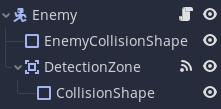
\includegraphics[width=5cm]{figures/screenshots/tree.png} }\label{fig:signal-example-a}}%
	\qquad
	\subfloat[\centering Signale]{{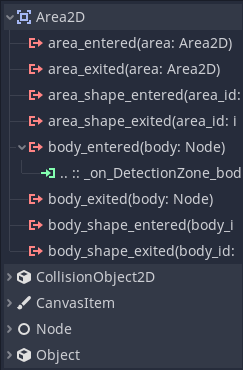
\includegraphics[width=5cm]{figures/screenshots/signals.png}
				\label{fig:signal-example-b}}}%
	\caption{Szenengraph und Signale der Area2D anhand eines Beispiels}%
	\label{fig:signal-example}%
\end{figure}

Die Godot Engine implementiert eine eigene Variante des Beobachtungsmusters\cite{godot-signals}\cite[293]{design-patterns-gof}.
Die Implementierung wird durch sogenannte Signale repräsentiert.
Jede Node besitzt Signale, welche von anderen Nodes beobachtet werden können.
\autoref{fig:signal-example} zeigt ein Beispiel, um dieses System zu verdeutlichen.
Der Szenengraph in \autoref{fig:signal-example-a} beinhaltet einen Gegner, welcher mit seiner Umgebung kollidieren kann.
Die \texttt{DetectionZone} vom Typ Area2D soll dem Gegner signalisieren, wenn ein Spieler diese Zone betritt.
Das Signal-Zeichen an der \texttt{DetectionZone}-Node symbolisiert, dass von dieser Node ein ausgehendes Signal existiert.
Dieses wird unter den verfügbaren Signalen (b) grün markiert. Ebenfalls ist zu sehen, dass neben den Signalen von Area2D noch viele weitere Signale existieren.
Parallel zu diesen, der nur für die vom Typ Area2D verfügbaren Signale, besitzt jede Node die Signale ihrer Elternklasse.
Area2D erbt von CollisionObject2D, welches von Node2D erbt. \\

Beim Auswählen eines Signals kann angegeben werden, welche Node das Signal empfängt und wie die Funktion benannt sein soll.
In diesem Fall handelt es sich um ein Signal vom Typ \texttt{body\_entered}.
Dieses wird ausgelöst, wenn eine Node vom Typ PhysicsBody2D die Area2D betritt.
Es sei angemerkt, dass mehrere Signale vom Typ \texttt{body\_entered} für eine Node existieren können.
Allerdings ist dies im angegebenen Beispiel nicht sinnvoll.
Eine Empfänger-Node muss ein Skript besitzen, weil ansonsten keine Zielfunktion angegeben werden kann.
Das Skript ist im Szenengraphen der Abbildung an der \texttt{Enemy}-Node zu erkennen.
Der Inhalt des Skripts befindet sich in \autoref{lst:signal}.\\

\definecolor{LightGray}{gray}{0.9}
\begin{listing}[H]
	\caption{Enemy.gd}
	\label{lst:signal}
	\begin{minted}[
bgcolor=LightGray,
framesep=2mm,
baselinestretch=1.2,
fontsize=\footnotesize,
linenos,
highlightlines={3}
]{gd.py:GDScriptLexer -x}
extends KinematicBody2D

func _on_DetectionZone_body_entered(body: PhysicsBody2D) -> void:
	_start_follow_player(body) # Pseudocode
\end{minted}
\end{listing}

Dieses Listing zeigt die Funktion, welche auf das Signal der Area2D reagieren soll.
Im Falle, dass ein Signal feuert, wird die Funktion aufgerufen, welche einem Spieler folgen soll.
Das Beispiel zeigt somit einen Gegner, welcher den Spieler automatisch verfolgt, sobald dieser sich in einem gewissen Radius befindet.\\

\begin{figure}[H]
	\centering
	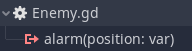
\includegraphics[width=0.4\columnwidth]{figures/screenshots/custom-signal.png}
	\caption{\label{fig:alarm} Benutzerdefiniertes Signal}
\end{figure}

Signale können ebenfalls im Code definiert und anschließend gefeuert werden.
Das vorherige Beispiel in \autoref{lst:signal} kann, wie in \autoref{lst:custom-signal} definiert, erweitert werden.
Das neue Signal erscheint dann im Editor und kann mithilfe der \texttt{connect}-Funktion oder dem Editor verbunden werden.
Der Gegner, welcher den Spieler gefunden hat, kann die globale Position als Parameter eines Signals feuern und weitere Gegner, welche auf dieses Signal hören, alarmieren.
Allerdings kann der Typ eines Signals in der ausgewählten Version der Godot Engine nicht angegeben werden.
Dies ist in Zukunft auch nicht geplant\cite{godot-signal-type}.
Aus diesem Grund ist der Typ des Signals in \autoref{fig:alarm} \texttt{var}.\\

\begin{listing}[H]
	\caption{Signale im Code}
	\label{lst:custom-signal}
	\begin{minted}
[
bgcolor=LightGray,
framesep=2mm,
baselinestretch=1.2,
fontsize=\footnotesize,
linenos,
highlightlines={3, 7},
]{gd.py:GDScriptLexer -x}
extends KinematicBody2D

signal alarm(position)

func _on_DetectionZone_body_entered(body: PhysicsBody2D) -> void:
	_start_follow_player(body) # Pseudocode
	emit_signal("alarm", body.global_position)
\end{minted}
\end{listing}

Das Problem an Signalen ist, dass diese bei einem wachsenden Projekt an vielen verschiedenen Stellen existieren und der Überblick verloren geht.
Um die Lösung für dieses Problem zu erklären, muss das von der Godot Engine implementierte Entwurfsmuster AutoLoad erläutert werden\cite{godot-autoload}.
AutoLoads sind eine Variation von Singletons\cite[S. 127]{design-patterns-gof}.
AutoLoads sind Skripte, welche beim Start der Anwendung automatisch global geladen werden.
Das bedeutet, dass sie in jeder Szene vorhanden sind.
Die Skripte können jeweils in den Projekteinstellungen konfiguriert werden.
Die Funktionsweise von AutoLoads ist nützlich, weil dadurch Code in allen anderen Skripten verfügbar ist.
Förderlich ist dies bei AutoLoads, welche zum Beispiel nur Konstanten enthalten.
Konstanten vom Typ String können verhindern, dass Tippfehler zu Fehlern führen.
Das liegt daran, dass alle Klassen, welche auf diese Konstanten zugreifen, dieselben Informationen erhalten.
Ebenfalls können auf diese Art und Weise global Minimal- oder Maximalwerte für bestimmte Variablen definiert werden.
Ein Beispiel hierfür ist die Maximalgeschwindigkeit jeder kinematischen Node, welche in einer Konstanten vom Typ Integer definiert ist.\\

\begin{listing}[H]
	\caption{Signale mit einem Eventbus}
	\label{lst:eventbus-signal}
	\begin{minted}
[
bgcolor=LightGray,
framesep=2mm,
baselinestretch=1.2,
fontsize=\footnotesize,
linenos,
highlightlines={5},
]{gd.py:GDScriptLexer -x}
extends KinematicBody2D

func _on_DetectionZone_body_entered(body: PhysicsBody2D) -> void:
	_start_follow_player(body) # Pseudocode
	EventBus.emit_signal("alarm", body.global_position)
\end{minted}
\end{listing}

Um das Problem von Signalen an unterschiedlichen Stellen im Code zu unterbinden, wurde ein Eventbus eingeführt\cite{dzone-eventbus}.
Dieses AutoLoad enthält mehrere Signale und die Skripte von Nodes können auf diese mit der \texttt{connect}-Funktion horchen.
Im Falle des erwähnten Beispiels könnte im Eventbus das Signal \texttt{alarm(position)} deklariert werden.
\autoref{lst:eventbus-signal} zeigt, wie ein Signal innerhalb einer Node über den Eventbus versendet werden kann.
Alle Nodes, welche auf dieses Event horchen, werden dann über ein aufgetretenes Signal über den Eventbus benachrichtigt.
Obwohl das Signal verwendet wird, wird die Warnung geworfen, dass das Signal nie benutzt wird.
Dies ist allerdings ein bekannter Fehler in der Spiel-Engine\cite{godot-signal-warning}.
Diese Warnung kann mithilfe eines Kommentars unterbunden werden. \\

\begin{listing}[H]
	\caption{Endlicher Automat}
	\label{lst:state-machine}
	\begin{minted}
[
bgcolor=LightGray,
framesep=2mm,
baselinestretch=1.2,
fontsize=\footnotesize,
linenos,
highlightlines={4-9, 12, 17},
]{gd.py:GDScriptLexer -x}
extends KinematicBody2D

var target: PhysicsBody2D
var state = IDLE
enum {
	IDLE,
	FOLLOW_PLAYER,
	WANDER,
}

func _physics_process(delta: float) -> void:
    _handle_state(delta)


func _on_DetectionZone_body_entered(body: PhysicsBody2D) -> void:
	target = body
	state = FOLLOW_PLAYER
	EventBus.emit_signal("alarm", body.global_position)
\end{minted}
\end{listing}

Ein weiteres Entwurfsmuster, welches in der Arbeit verwendet wird, ist das Entwurfsmuster eines endlichen Automaten\cite{gamepattern-state}.
Voraussetzung für diesen sind eine endliche Menge an Zuständen.
Im Beispiel \autoref{lst:state-machine} existieren die Zustände \texttt{IDLE}, \texttt{FOLLOW\_PLAYER} und \texttt{WANDER}.
Die Mächtigkeit dieser Menge ist drei, was bedeutet, dass sie endlich ist.
Verwendet werden solche Zustände, um Programmlogik zu separieren und Aktionen nur bestimmten Zuständen verfügbar zu machen.
Im Beispiel wechselt der Gegner zwischen den Zuständen \texttt{IDLE} und \texttt{WANDER} hin und her.
Das bedeutet, dass der Gegner entweder auf seiner Position stehen bleibt oder die Gegend erkundet.
Wenn ein Spieler die \texttt{DetectionZone} betritt, wird der Zustand auf \texttt{FOLLOW\_PLAYER} (Spieler folgen) gesetzt.
Mithilfe weiterer Funktionen kann diese Logik so umgeschrieben werden, dass der Gegner dem Spieler nur über eine bestimmte Distanz folgt und dann zum \texttt{IDLE}-Zustand zurückkehrt.\\

\subsection{Besondere Funktionalitäten}
Die Godot Engine bietet neben den vorgestellten Entwurfsmustern weitere nützliche Funktionalitäten und Schlüsselwörter. Die Funktion \texttt{ready} wird aufgerufen, wenn eine Node den Szenengraph betritt. In dieser Funktion werden üblicherweise Variablen initialisiert, Animationen gestartet oder Signale gefeuert. \\

Die Funktion \texttt{process} wird bei jedem Frame aufgerufen. Das bedeutet, dass die Häufigkeit davon abhängt, mit wie vielen Bildern pro Sekunde (\ac{FPS}) die Anwendung läuft. Die Funktion \texttt{physics\_process} funktioniert ähnlich, allerdings hängt die Häufigkeit der Ausführung von der im Editor eingestellten Physics-\ac{FPS} ab. Das Problem ist nun, dass beide Funktionen von einem Lag beeinflusst werden können. Ein Lag ist eine Verzögerung und sorgt dafür, dass die Anzahl an \ac{FPS} sinken kann. Das kann dazu führen, dass die Häufigkeit, wie oft eine Funktion ausgeführt wird, sinken kann. Die Ursache dafür sind meistens andere Applikation, Hardware-Ressourcen oder mangelnde Optimierung in der eigenen Applikation. Eine Lösung für dieses Problem bietet die Spiel-Engine mithilfe des Parameters \texttt{delta}.\\

Durch den Parameter \texttt{delta} kann die Berechnung abhängig der Schwankung der \ac{FPS} durchgeführt werden. Dieser Wert gibt die vergangene Zeit der Ausführung der Funkion an. Der Grund, wieso dies nützlich ist, wird an einem Beispiel deutlich. Der Parameter \texttt{delta} gibt bei 60 \ac{FPS} also $\frac{1}{60}$ Sekunde pro Frame an. Falls sich die \texttt{FPS} aufgrund von Lag halbieren sollten, beträgt \texttt{delta} $\frac{1}{30}$ Sekunde pro Frame. Es seien zwei Funktionen gegeben, wobei $delta_0 = \frac{1}{60} \frac{s}{frame}$ und $delta_1 = \frac{1}{30} \frac{s}{frame}$ sind.\\

\setcounter{equation}{0}
\begin{equation}
    60 \frac{m}{s} \cdot delta_0 = 1 \frac{m}{frame}
\end{equation}

\begin{equation}
  60 \frac{m}{s} \cdot delta_1 = 2 \frac{m}{frame}
\end{equation}

Anhand dieser Funktionen wird deutlich, dass wenn die \ac{FPS} um einen Faktor zwei geringer wird, die Geschwindigkeit mit der sich ein Node bewegt, um den Faktor zwei erhöht werden muss. Das Ergebnis davon ist, dass in gleicher Zeit die gleiche Distanz zurückgelegte wird. Allerdings ist die Konsequenz daraus, dass eine Bewegung abgehackt wirkt.

\begin{listing}[H]
\caption{Dollar-Zeichen}
\label{lst:dollar}
\begin{minted}
[
bgcolor=LightGray,
framesep=2mm,
baselinestretch=1.2,
fontsize=\footnotesize,
linenos,
]{gd.py:GDScriptLexer -x}
var shape: CollisionShape2D

func _ready() -> void:
	shape = $EnemyCollisionShape
\end{minted}
\end{listing}

Es ist in der Spiel-Engine oftmals erforderlich, von einem Skript aus auf Knoten weiter unten in der Hierarchie zuzugreifen. Üblicherweise wird dafür die Funktion \texttt{get\_node(``NodePath'')} verwendet, wobei NodePath der relative Pfad zum Zielknoten ist. Weil dies allerdings häufig vorkommt, kann diese Funktion mit einem Dollar-Zeichen abgekürzt werden und ist in \autoref{lst:dollar} zu sehen.

\begin{listing}[H]
\caption{Schlüsselwort onready}
\label{lst:onready}
\begin{minted}
[
bgcolor=LightGray,
framesep=2mm,
baselinestretch=1.2,
fontsize=\footnotesize,
linenos,
highlightlines={1},
]{gd.py:GDScriptLexer -x}
onready var shape: CollisionShape2D = $EnemyCollisionShape

func _ready() -> void:
	pass
\end{minted}
\end{listing}

Eine weitere Abkürzung ist das Schlüsselwort \texttt{onready}. Die Variable \texttt{shape} kann nicht bereits beim Deklarieren zugewiesen werden, weil die Node \texttt{EnemyCollisionShape} den Szenengraph noch nicht betreten hat. Damit dies möglich wird, kann das Schlüsselwort \texttt{onready}, wie in \autoref{lst:onready}, vor die Variable geschrieben werden.\\

Das Schlüsselwort \texttt{export} macht Variablen im Editor sichtbar. Dort können Werte zugewiesen oder Referenzen zu anderen Nodes gespeichert werden. Um eine Szene im Voraus laden zu können, kann statt dem Schlüsselwort \texttt{load} das Schlüsselwort \texttt{preload} verwendet werden.

\begin{listing}[H]
\caption{Schlüsselwort setget}
\label{lst:setget}
\begin{minted}
[
bgcolor=LightGray,
framesep=2mm,
baselinestretch=1.2,
fontsize=\footnotesize,
linenos,
highlightlines={1, 4-5, 10},
]{gd.py:GDScriptLexer -x}
var value: int setget set_value, get_value

func _ready() -> void:
	value = 4 
	self.value = 2


func set_value(new_value):
	value = new_value
	EventBus.emit_signal("value", new_value)


func get_value():
	return value
\end{minted}
\end{listing}

Set- und Get-Methoden werden in den meisten Programmiersprachen verwendet, um Daten zu kapseln. Ebenfalls können diese um weitere Funktionalitäten erweitert werden, welche ausgelöst werden, wenn ein Variablenwert sich verändert. Die Godot Engine bietet mithilfe des \texttt{setget}-Schlüsselworts eine Möglichkeit, diese Set- und Get-Methoden zu definieren. Dabei sei angemerkt, dass diese Methoden nur ausgelöst werden, wenn ein Zugriff von einem externen Skript erfolgt oder das Schlüsselwort \texttt{self} verwendet wird. Ein lokaler Zugriff auf die Variable löst die Set- und Get-Methoden nicht aus.
\subsection{Implementation}
Bevor die in \autoref{sec:wireframes} entwickelten Konzepte realisiert werden, muss das Projekt in der Godot Engine konfiguriert werden.
Im Anschluss werden Kernmechaniken, wie Bewegung des Charakters oder des Partners, realisiert.
Auf diesen Grundlagen können dann die ermittelten Hypothesen implementiert werden.
Dieser Vorgang wird in diesem Abschnitt beschrieben.
Das Spiel trägt den Titel \texttt{EvoWorld} und ist als 2D-Pixel-Art-Spiel ausgearbeitet.

\subsubsection{Konfiguration}
Aufgrund der Tatsache, dass es sich um ein Spiel in Pixel-Grafik handelt, ist die Fenstergröße dementsprechend konfiguriert.
In der Projekteinstellungen der Godot Engine ist die Größe auf 320x180 eingestellt.
Diese wird später künstlich auf 1280x720 hochskaliert.
Ebenfalls müssen Einstellungen in dem Physik-Modul vorgenommen werden.
Das Kollisionsystem der Godot Engine basiert auf einem Schichtsystem\cite{godot-collision}.
Das bedeutet, dass ausgewählt werden kann, auf welcher Kollisionsebene sich ein CollisionObject2D befindet.
Der \texttt{Layer} gibt an, auf welcher Ebene sich das Objekt befindet und eine \texttt{Mask} gibt an, mit welcher Ebene dieses kollidieren kann.
Im Projekt sind vier verschiedene Ebenen spezifiziert.\\

Die World-Ebene gibt an, welche Kollisionsobjekte sich in der Welt befinden.
Ein Beispiel dafür sind Wände, welche nicht von Spielenden, Gegnern oder \ac{NPC} passierbar sind.
Drei weitere Ebenen sind die Player-, Enemy- und \ac{NPC}-Ebene.
Die Player-Ebene ist nötig, um bestimmte Funktionen auszulösen.
Beispielhaft wäre eine Kollision des Hauptcharakters auf der Player-Ebene mit einem Gegner auf der Enemy-Ebene.
Dies resultiert in einem Kampf.
Die \ac{NPC}-Ebene wird dafür verwendet, dem Hauptcharakter eine Interaktion mit den \ac{NPC} zu ermöglichen.

\subsubsection{Assets}
Assets sind nicht-technische Inhalte, welche in Videospielen verwendet werden.
Diese können in Form von Sprites, Animationen oder Musik existieren.
Ebenfalls lassen sich noch weitere Elemente unter diesem Oberbegriff kategorisieren.
Der Fokus lag in der Arbeit allerdings auf visuellen Assets in Form von Sprites.
Für diesen Zweck entstand eine interdisziplinäre Kooperation mit einer Game Art \& 3D Animation Studentin des SAE Instituts\cite{sae-institute}.
Diese Kooperation ist aufgrund zeitlicher Probleme pausiert und kann erst nach der Arbeit fortgesetzt werden.
Zwei Assets sind innerhalb dieser Kooperation entstanden.
Das Sprite des Hauptcharakters und eines Gegners.
Alle weiteren Sprites sind selbst entwickelt.
Lediglich die Schriftart \texttt{NESCyrillic} ist noch ein weiteres externes Asset.
Alle Lizenzen und Referenzen zu den Inhalten sind in der \texttt{README.md} des Projekts angegeben.

\subsubsection{Bewegung}
Eine wichtige Kernmechanik eines Rollenspiels ist die Bewegung des Charakters.
Die Bewegung erfolgt anhand der \texttt{WASD}-Tasten.
Die Eingabe wird als zweidimensionaler Vektor interpretiert.
Je nach Taste wird der X- oder Y-Wert um eins addiert oder subtrahiert.
Die Interpretation wird dann auf den Charakter angewandt, welcher sich dann in Geschwindkeit und Richtung des Vektors bewegt.
Beim Drücken der Taste \texttt{D} entsteht der Vektor $(1, 0)$ und die Länge des Vektors beträgt eins.
Dieser Vektor ist als $\vec{v}$ in \autoref{fig:distance} gekennzeichnet.\\

% 0,0 URSPRUNG
\begin{figure}[ht]
    \centering
    \scalebox{1.5}{
        \begin{tikzpicture}
            \tkzInit[xmax=1,ymax=1]
            \tkzDefPoint (1,0){A}
            \tkzDefPoint (1,1){B}
            \tkzDefPoint (0,1){C}
            \tkzDrawXY
            \tkzGrid
            \draw [red,thick,opacity=0.7, domain=0:90] plot ({cos(\x)}, {sin(\x)});
            \tkzLabelPoint[blue,above right](A){$(1,0)$}
            \tkzLabelPoint[blue, above right](B){$(1,1)$}
            \tkzDrawPoints[blue](A, B)
            \draw[line width=1pt, black, -stealth](0, 0) -- (1,1) node[midway, above]{$\vec{u}$};
            \draw[line width=1pt, black, -stealth](0, 0) -- (1,0) node[midway, below]{$\vec{v}$};
        \end{tikzpicture}
    }
    \caption{Distanz und Einheitskreis}
    \label{fig:distance}
\end{figure}

Diese Methodik birgt allerdings ein Problem.
Wenn die spielende Person zwei Eingaben auf unterschiedlichen Achsen tätigt, kann es dazu kommen, dass die Länge des Vektors nicht gleich eins beträgt.
Das liegt daran, dass die Länge eines Vektors als folgende Funktion gegeben ist\cite[S.16]{vector-math}.

\setcounter{equation}{0}
\begin{equation}
    |\vec{a}| = |\left(\begin{array}{c} a_1 \\ a_2 \end{array}\right)| = \sqrt{a_1^2 + a_2^2}
\end{equation}

Wenn eine Person nun zusätzlich zu der Taste \texttt{D} die Taste \texttt{S} betätigt, entsteht der Vektor $(1, 1)$.
Wie in der \autoref{fig:distance} zu sehen, ist die Länge des Vektors $\vec{u}$ größer als die des Vektors $\vec{v}$.
Die Länge von $\vec{u}$ beträgt nämlich $\sqrt{2}$.
Das bedeutet, dass eine Bewegung in der Diagonale schneller wäre, als eine Bewegung entlang einer der beiden Achsen.
Das Problem kann allerdings umgangen werden, wenn dieser Vektor normiert wird\cite[S.22]{vector-math}.
Dies sorgt dafür, dass der Vektor auf die Länge des Radius vom Einheitskreises reduziert wird, welcher in rot eingezeichnet ist.
Dieser Radius beträgt eins.\\

Damit der Charakter langsam beschleunigt, wird die \texttt{move\_toward}-Funktion verwendet\cite{godot-move-toward}.
Diese erhöht oder verringert einen Vektor bezüglich eines anderen Vektors in Abhängigkeit von \texttt{delta}.
Ebenfalls wird diese Funktion verwendet, um den Charakter bei keiner Eingabe langsam auzubremsen.
Die \texttt{move\_and\_slide}-Funktion sorgt dann dafür, dass sich dieser in Richtung des Vektors bewegt\cite{godot-move-and-slide}.
Falls der Charakter mit einer CollisionShape2D kollidiert, stoppt dieser nicht, sondern gleitet an der Form der CollisionShape2D entlang.\\

Ein RayCast2D gibt die Rotation des Charakters an.
Diese wird mithilfe der Funktion \texttt{atan2} und dem Eingabevektor als Übergabeparameter berechnet\cite{godot-builtins}.
Das Resultat ist der Polarwinkel $\varphi$, welcher die aktuelle Rotation in Radiant angibt.\\

\subsubsection{Menüs}
Im Rahmen des Projekts sind mehrere Menüs und ein Pop-up entwickelt worden.
Das Startmenü ermöglicht es, den Spielenden auszuwählen, ob diese mit dem Spiel beginnen möchten oder zunächst Einstellungen vornehmen wollen.
Es existiert zwar ein Einstellungsmenü, allerdings ist dieses nicht technisch implementiert.
Das liegt daran, dass der Fokus zunächst auf das Gameplay gelegt ist.
Das erwähnte Pop-up ist das Fenster, welches angezeigt wird, wenn die spielende Person einen Kampf verliert und ihr die verlorenen Gegenstände mitgeteilt werden sollen. \\

\begin{figure}[H]
    \centering
    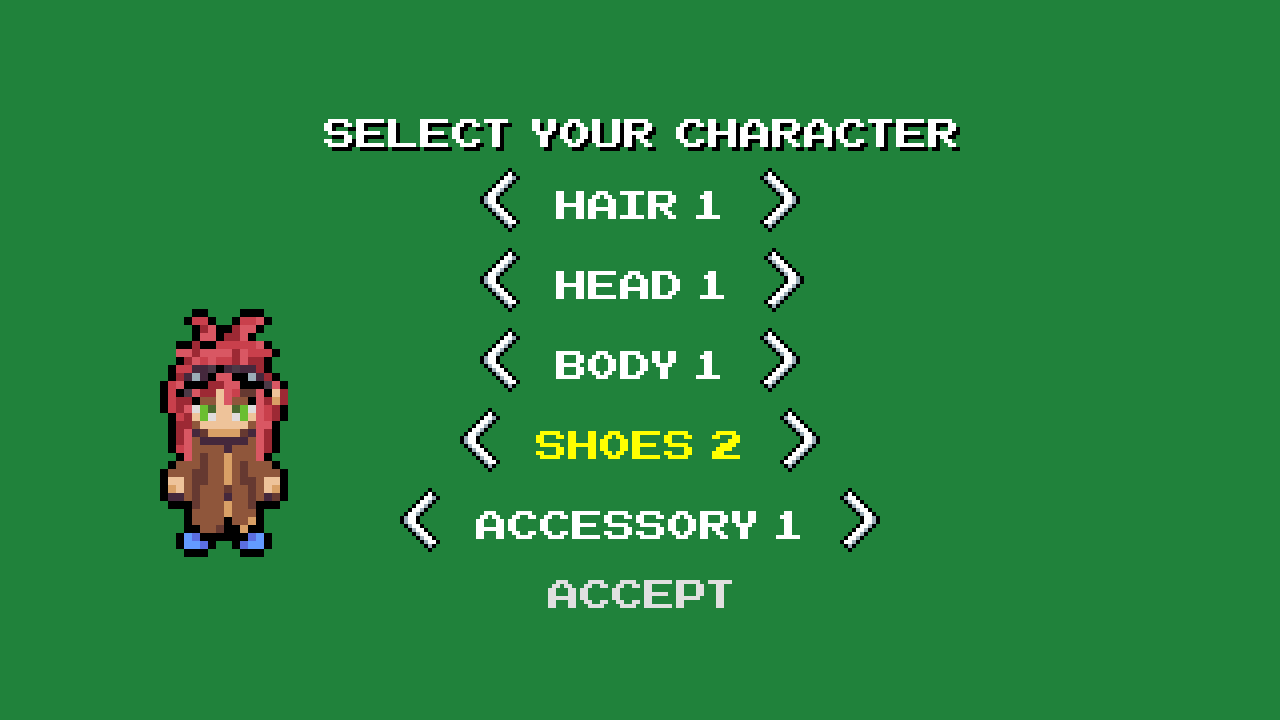
\includegraphics[width=0.8\columnwidth]{figures/screenshots/charselect.png}
    \caption{\label{fig:char-impl}Charakterauswahlmenü}
\end{figure}

Wenn die spielende Person das Spiel beginnt, landet diese zunächst im Charakterauswahlmenü.
Dieses Menü ist in \autoref{fig:char-impl} dargestellt und nach dem in \autoref{sec:wireframes} vorgestellten Wireframe modelliert.
Die Szene ist primär mithilfe von Control-Nodes aufgebaut.
Allerdings befindet sich innerhalb dieser Control-Nodes die Node des Hauptcharakters.
Diese ist zusammengesetzt aus verschiedenen Sprite-Nodes, welche die einzelnen Körperteile repräsentieren.
Beim Wechsel der einzelnen Komponenten wird die Funktion \texttt{\_on\_button\_pressed} im Skript des Menüs ausgelöst.
Dies sorgt dafür, dass die Zahl hinter der Bezeichnung eines Elements angepasst und die Informationen über die aktuelle Auswahl dem \texttt{Player}-Node übergeben wird.
Dort werden die entsprechenden Sprites angezeigt, welche bereits vom Skript \texttt{sprites.gd} mithilfe von \texttt{preload} vorgeladen sind.
In Hinblick auf die weitere Entwicklung nach dieser Arbeit werden diese Daten ebenfalls in einem Autoload-Skript gespeichert.
Diese können dann an unterschiedlichen Orten geladen werden, um die \texttt{Player}-Node mit den zuvor gespeicherten Sprites zu laden.
Nach Betätigen des \texttt{Accept}-Knopfes landet die spielende Person im Spiel. \\

\begin{figure}[H]
    \centering
    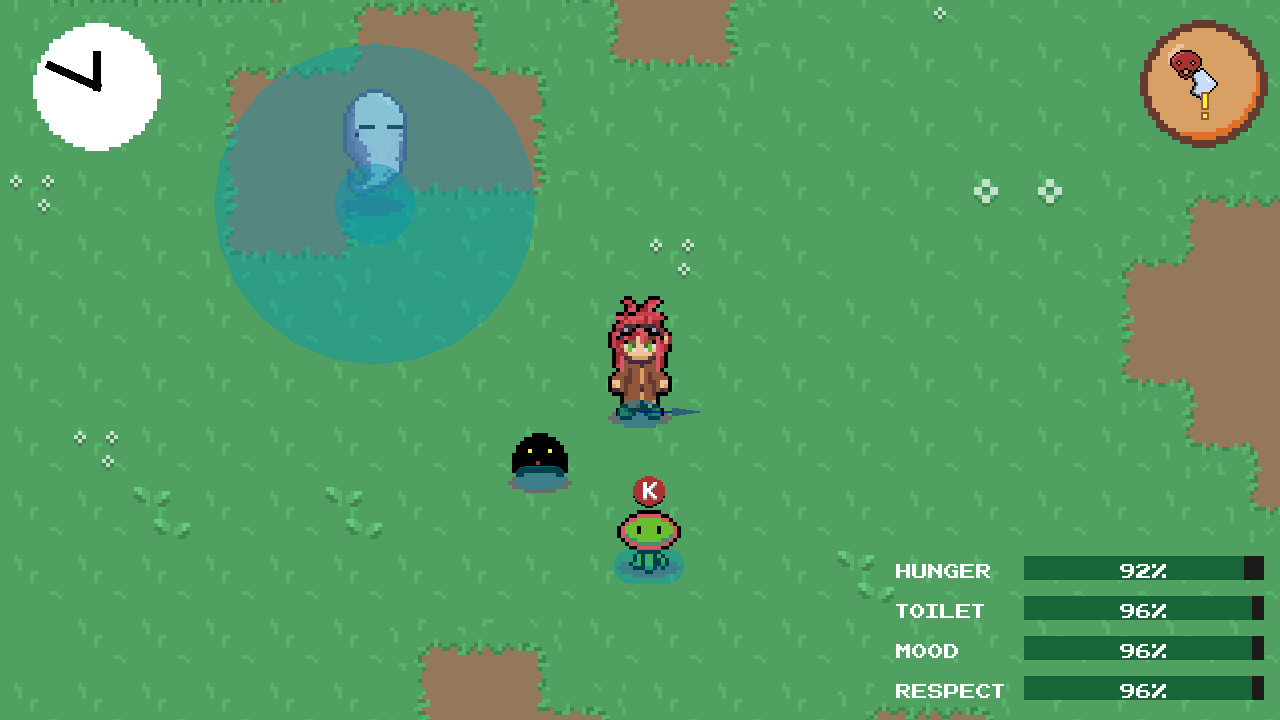
\includegraphics[width=0.8\columnwidth]{figures/screenshots/ingame.png}
    \caption{\label{fig:ingame}Innerhalb der Spielwelt}
\end{figure}

\autoref{fig:ingame} zeigt den Spielinhalt, wenn eine spielende Person den Charakter ausgewählt hat.
Diese Abbildung enthält mehrere Informationen, welche im Folgenden erklärt werden.
Die blauen Kreise um einzelne Objekte sind CollisionShapes, welche aktiviert sind, um die Inhalte des Spiels besser erklären zu können.
Als Erstes wird das \ac{HUD} näher beschrieben.
Dieses ähnelt dem \ac{HUD} in Digimon World, mit dem Zusatz, dass eine Minimap und weitere Fortschrittsbalken existieren.
Ebenfalls ist die Uhr als 12-Stunden-Anzeige mit zwei Zeigern modelliert.\\

Die Karte ist anhand eines Tutorials implementiert\cite{kids-minimap}.
Dieses Tutorial ist verwendet worden, weil es dem Entwurf in \autoref{sec:wireframes} entspricht.
Jedes Objekt, welches in der Minimap vorkommt, besitzt die Variable \texttt{minimap\_icon}, welche dafür zuständig ist, das Objekt mit dem korrekten Symbol auf der Karte einzublenden.
Alle Nodes, welche diese Eigenschaft besitzen, werden der Gruppe \texttt{minimap\_objects} zugeordnet.
\autoref{lst:group} zeigt die Möglichkeit, mithilfe von Gruppen alle Nodes zu filtern, welche sich in der Gruppe \texttt{minimap\_objects} befinden und im Szenengraph vorhanden sind.\\

\begin{listing}[H]
    \caption{Nodes innerhalb einer Gruppe}
    \label{lst:group}
    \begin{minted}
[
bgcolor=LightGray,
framesep=2mm,
baselinestretch=1.2,
fontsize=\footnotesize,
linenos,
]{gd.py:GDScriptLexer -x}
var map_objects = get_tree().get_nodes_in_group("minimap_objects")
\end{minted}
\end{listing}

Eine neue Aufgabe besitzt den Wert \texttt{quest} und ist als gelbes Ausrufezeichen modelliert.
Gegner besitzen den Wert \texttt{enemy} und sind als rote Totenkopfschädel modelliert.
Objekte außerhalb des sichtbares Bereiches werden am Rande der Karte verkleinert dargestellt.
Ebenfalls ist es möglich, mithilfe des Mausrads das Zoomlevel der Karte einzustellen. \\

\begin{figure}[H]%
    \centering
    \subfloat[\centering Aufgabenliste]{{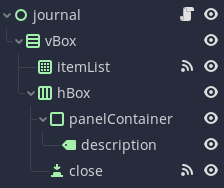
\includegraphics[width=5cm]{figures/screenshots/journal.png} }\label{fig:journal-a}}%
    \qquad
    \subfloat[\centering Inventar]{{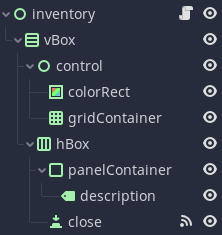
\includegraphics[width=5cm]{figures/screenshots/inventory.png}
                \label{fig:inventory-b}}}%
    \caption{Aufgabenliste und Inventar}%
    \label{fig:inventory-journal-impl}%
\end{figure}

\autoref{fig:inventory-journal-impl} verdeutlicht den Szenengraphen der Aufgabenliste und des Inventars.
Die Beschreibung und der \texttt{Schließen}-Knopf haben in beiden Fällen dieselbe Funktionalität.
Die Beschreibung gibt Details über eine Aufgabe oder einen Gegenstand an, welcher aktuell selektiert ist.
Mithilfe eines Signals des Knopfes wird das Event \texttt{close\_button\_pressed} gefeuert, welches dafür sorgt, dass ein aktives Fenster geschlossen wird. \\

Die Aufgabenliste in \autoref{fig:journal-a} ist anhand einer ItemList implementiert\cite{godot-itemlist}.
Diese beinhaltet eine Spalte, der Elemente hinzugefügt werden können.
Falls die Liste zu viele Elemente enthält, um alle darzustellen, wird eine Scrollleiste hinzugefügt.
Die ItemList besitzt das Signal \texttt{item\_selected}, welches gefeuert wird, wenn ein Element in der Liste ausgewählt wird.
Innerhalb des Skripts \texttt{journal.gd} wird die Beschreibung dann durch die Beschreibung des jeweiligen Elements ersetzt.\\

Das Inventar hingegen ist mit einem GridContainer konstruiert worden\cite{godot-gridcontainer}.
Dies ist in \autoref{fig:inventory-b} zu sehen.
Der GridContainer besitzt eine feste Anzahl von Reihen und Spalten.
Ebenfalls ist der Hintergrund durchsichtig.
Aus diesem Grund wird ein ColorRect verwendet, um die Hintergrundfarbe zu definieren\cite{godot-colorrect}.
Die feste Anzahl wurde hier verwendet, um den Platz des Inventars zu begrenzen.
Die einzelnen Aufgaben oder Gegenstände sind ebenfalls in Hinblick auf die Zukunft innerhalb der \texttt{PlayerVariables} gespeichert.\\

Die Statuswerte des Partners, welche in \autoref{fig:ingame} dargestellt sind, werden durch Prozentzahlen repräsentiert.
Dies soll helfen, die aktuelle Lage besser einschätzen zu können, statt diese Werte nur anhand der Fortschrittsbalken abzuschätzen.
Ebenfalls besitzt jeder Fortschrittbalkens ein Label, welches diesen beschreibt.
Die Werte werden aktuell mithilfe eines Timers und nach einem bestimmten Intervall weniger.
Diese Änderung wird dann mithilfe des Signals \texttt{status\_changed} über den Eventbus gefeuert. \\

\subsubsection{Non-player character}\label{sec:npc}
Die in \autoref{fig:ingame} abgebildete Blume ist ein ansprechbarer \ac{NPC}.
Dieser besitzt eine \texttt{triggerZone}, welche ein Signal feuert, wenn die spielende Person diese betritt.
Die Auswirkung davon ist, dass der Interaktionsknopf über dem Sprite des \ac{NPC} zu sehen ist. \\

\begin{listing}[H]
    \caption{RayCast Interaktion mit einem \ac{NPC}}
    \label{lst:handle-colliding}
    \begin{minted}
[
bgcolor=LightGray,
framesep=2mm,
baselinestretch=1.2,
fontsize=\footnotesize,
linenos,
]{gd.py:GDScriptLexer -x}
func _handle_colliding() -> void:
	if !Input.is_action_just_pressed("confirm"):
		return
		
	if !ray.is_colliding():
		return
	
	var target = ray.get_collider().get_parent()
	EventBus.emit_signal("confirm_button_pressed", target)
\end{minted}
\end{listing}

\autoref{lst:handle-colliding} beschreibt die technische Umsetzung, um mit diesem \ac{NPC} zu interagieren.
Zunächst muss die spielende Person die Taste \texttt{K} betätigen.
Ebenfalls muss der RayCast2D mit einem \ac{NPC} kollidieren.
Das bedeutet, dass die spielende Person sehr nah stehen und in die Richtung des \ac{NPC} schauen muss.
Hierfür wurden Kollisionsmasken verwendet, um sicherzustellen, dass nur interagierbare Objekte mit dem RayCast2D kollidieren können.
Falls beide Konditionen erfüllt sind, wird das interagierbare Objekt über den Eventbus als Signal verschickt.
Jede \ac{NPC}-Node hört auf dieses Signal und validiert, ob \texttt{target} mit der Node übereinstimmt.
Falls dies der Fall ist, wird ein Dialog gestartet.

\subsubsection{Dialoge}
Dialoge sind mithilfe der Erweiterung Dialogic umgesetzt\cite{github-dialogic}.
Diese Erweiterung fügt einen weiteren Reiter mit dem gleichen Namen im Editor hinzu.
In dieser Komponente können Dialoge entsprechend konfiguriert werden.
Beispielhaft wird der Dialog mit der in \autoref{sec:npc} erwähnten Blume näher erläutert.\\

\begin{figure}[H]
    \centering
    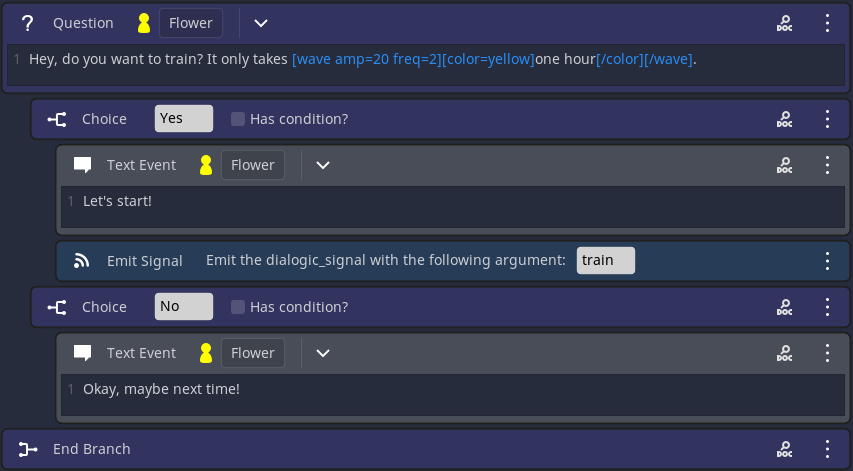
\includegraphics[width=0.9\columnwidth]{figures/screenshots/dialogic.png}
    \caption{\label{fig:dialogic}Dialog mit dem \ac{NPC} Flower}
\end{figure}

Der in \autoref{fig:dialogic} dargestellte Dialog wird in Dialogic mithilfe einer Timeline umgesetzt.
Eine Timeline ist eine Abfolge von Events. Diese können Texte, bestimmte Konditionen, Signale oder weitere Events beinhalten.
In diesem Beispiel wird zunächst eine Frage gestellt, auf welche die spielende Person mit \texttt{Ja} oder \texttt{Nein} antworten kann.
Für den Fall, dass die Option \texttt{Ja} gewählt wird, wird das Signal \texttt{train} gefeuert, welches dafür sorgt, dass eine Stunde im Spiel vergeht.
Für den Fall, dass die Option \texttt{Nein} gewählt wird, passiert nichts.
In beiden Fällen wird nach auflösen der Events die Konversation beendet.
Die Texte können mithilfe von BBCode modifiziert werden.
Dies ist im ersten Event in der Abbildung zu sehen.
Dort wird eine Animation und eine farbliche Kennzeichnung für einen bestimmten Abschnitt im Text angewandt.

\subsubsection{Bewegung des Partners}
Im Referenzspiel Digimon World folgt das Partner-Digimon dem Spieler automatisch.
In der in dieser Arbeit implementierten Variante ist dies ebenfalls der Fall.
Die Bewegung des Partners zur spielenden Person erfolgt anhand linearer Interpolation.
Lineare Interpolation beschreibt in diesem Fall den Wechsel zwischen zwei Positionen $P$ und $S$.
Der Parameter $i$  gibt dabei die aktuelle Interpolation an, wobei $i$ zwischen Null und Eins liegt.
Wenn $i=0{,}5$ beträgt, befindet sich die aktuelle Position in der Mitte zwischen $P$ und $S$.
Mithilfe der, von der Godot Engine bereitgestellten, Funktion \texttt{linear\_interpolate} kann die beschrieben Interpolation umgesetzt werden.
Dafür wird als Zielposition die Position des Hauptcharakters gewählt und die Interpolation errechnet sich aus \texttt{delta} multipliziert einer konstanten Geschwindigkeit. \\

\subsubsection{Bewegung des Gegners}
Die Bewegungsmuster des Gegners sind mithilfe eines endlichen Automaten realisiert.
\autoref{fig:fsm} zeigt alle möglichen Zustände an, welche ein Gegner annehmen kann.
Die Zustandswechsel erfolgen unter drei verschiedenen Bedingungen.
Der Hauptcharakter hat die in \autoref{fig:ingame}, um den Gegner markierte, \texttt{triggerZone} betreten oder verlassen, eine bestimmte Distanz zu einem Zielpunkt ist erreicht oder ein Timer ist abgelaufen.
Der Zustand \texttt{WANDER} ($w$) ist als Initalzustand festgelegt.
In diesem Zustand bewegt sich der Gegner auf einen zufällig ausgewählten Zielpunkt innerhalb eines bestimmten Radiuses zu.
Wenn dieser eine bestimmte Distanz zum Zielpunkt erreicht oder das Signal des Timers \texttt{\_on\_timer\_timeout} feuert, wechselt der Zustand in den \texttt{STOP}-Zustand ($s$).
Direkt zurück in den Zustand $w$ kommt der Gegner nur, wenn das Signal des Timers erneut gefeuert wird.
Dieses Verhalten soll einen Gegner simulieren, welcher in einem bestimmten Radius umherwandert. \\

\tikzset{
->,
node distance=3cm, .
every state/.style={thick, fill=gray!10},
initial text=$ $,
}


\begin{figure}[H]
    \centering
    \begin{tikzpicture}
        \node[state, initial] (w) {$w$};
        \node[state, right of=w] (s) {$s$};
        \node[state, below of=w] (m) {$m$};
        \node[state, right of=m] (c) {$c$};
        \node[state, accepting, right of=c] (f) {$f$};
        \draw (w) edge[right] node{trigger} (c);
        \draw (c) edge[above, bend right] node{trigger} (m);
        \draw (m) edge[above, bend right] node{trigger} (c);
        \draw (m) edge[left] node{distance} (w);
        \draw (w) edge[above] node{distance} (s);
        \draw (w) edge[above, bend left] node{timer} (s);
        \draw (s) edge[above, bend left] node{timer} (w);
        \draw (s) edge[right] node{trigger} (c);
        \draw (c) edge[above] node{fight} (f);
    \end{tikzpicture}
    \caption{Nichtdeterministischer endlicher Automat}
    \label{fig:fsm}
\end{figure}

Beide Zustände können mithilfe des Signals \texttt{\_on\_triggerZone\_player\_entered} der \texttt{triggerZone} in den Zustand \texttt{CHASE\_PLAYER} ($c$) wechseln.
Wenn der Gegner in diesem Zustand ist, bewegt er sich auf den Hauptcharakter zu.
Sollte es zu einer Kollision mit dem \texttt{fightTrigger} kommen, wird das Signal \texttt{combat\_started} über den Eventbus gefeuert.
Anschließend findet ein Kampf statt und der Automat erreicht den Endzustand $f$.
Für den Fall, dass die Distanz zum Hauptcharakter größer als ein festgelegter Wert ist, wird der Zustand auf \texttt{MOVE\_BACK} ($m$) gesetzt.
Dabei wird erneut das Signal \texttt{\_on\_triggerZone\_player\_entered} gefeuert.
In diesem Fall ist der Wert des Signals allerdings \texttt{false}.
Im Zustand ($m$) bewegt sich der Gegner zur Startposition zurück.
Sollte die Spielende Person die \texttt{triggerZone} erneut auslösen, verfolgt der Gegner den Hauptcharakter erneut.
Wenn allerdings die Startposition erreicht wird, wandert der Gegner erneut umher.\\

\subsubsection{Kampf}
\autoref{fig:combat} stellt eine Kampfsituation dar.
Diese ist nach dem Entwurf in \autoref{fig:battle-wireframe} modelliert.
Sie besitzt allerdings einige technische Besonderheiten, welche in diesem Abschnitt erklärt werden.

\begin{figure}[H]
    \centering
    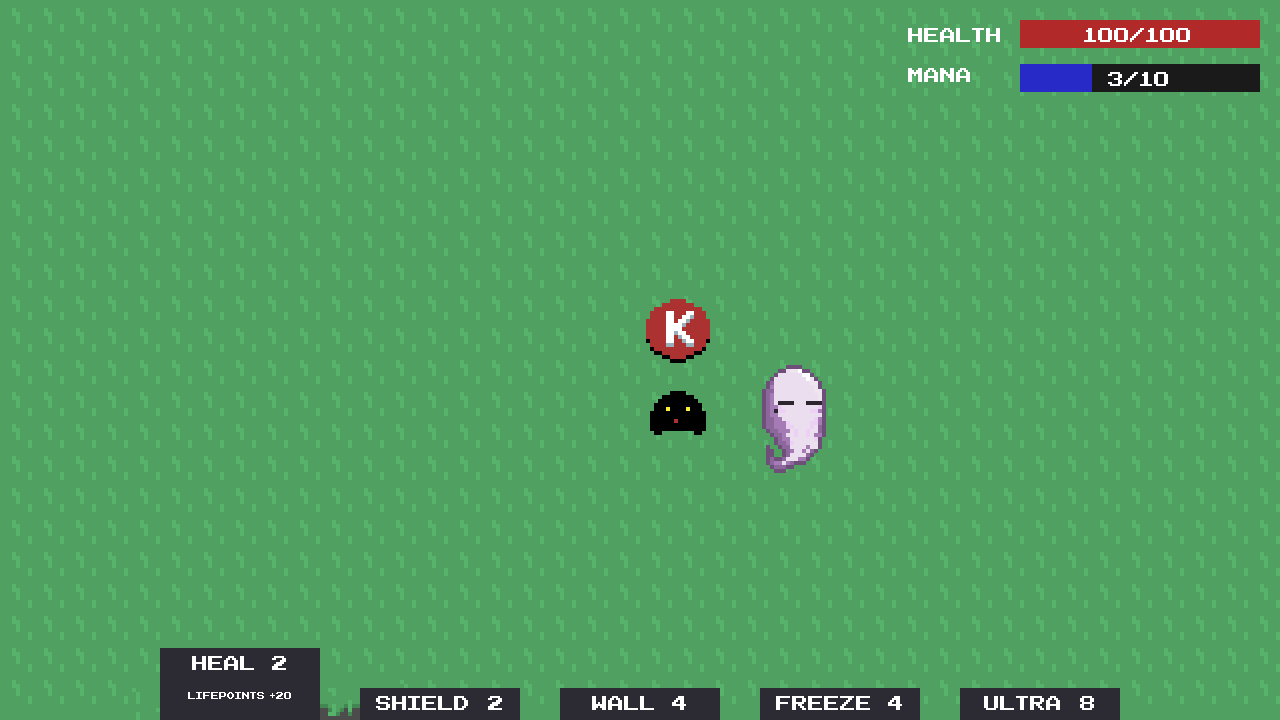
\includegraphics[width=0.8\columnwidth]{figures/screenshots/combat.png}
    \caption{\label{fig:combat}Kampfszene}
\end{figure}

Zunächst sind die Szenengraphen für \texttt{Pet} und \texttt{Enemy} als eine neue Szene abgebildet.
Die Szene \texttt{CombatEntity}, welche als Ersatz für beide Entitäten dient, wird an dieser Stelle verwendet, um den Entwicklungsprozess zu beschleunigen.
Das liegt daran, dass ansonsten Werte zwischengespeichert und in eine neue Szene übertragen werden müssten.
Ebenfalls müsste das Skript für beide Nodes stark angepasst werden.
Der Unterschied zwischen den beiden Entitäten wird im Skript mithilfe eines Booleans repräsentiert.
Das bedeutet, dass einige Zeilen Code nur für das \texttt{Pet} ausgeführt werden.\\

In einem Kampf bewegen sich beide Entitäten aufeinander zu.
Dies geschieht mithilfe den vorher erwähnten Funktionen \texttt{move\_towards} und \texttt{move\_and\_slide}.
Wenn eine gewisse Distanz zwischen beiden Entitäten erreicht ist, wird die Zeit mithilfe des Parameters \texttt{time\_scale} des \texttt{Engine}-Singletons heruntergesetzt\cite{godot-class-engine}.
Das Resultat ist, dass die Zeit im Spiel langsamer verläuft.
Danach wird ein Timer gestartet, welcher die Zeit wieder zurücksetzt.
Während dieser Timer läuft, wird der spielenden Person die Taste \texttt{K} angezeigt, welche geklickt werden kann, um Mana im Kampf zu generieren. \\

Aufgrund der Tatsache, dass beide Entitäten aufeinander zulaufen, kommt es ab einem gewissen Zeitpunkt zu einem Kontakt.
Wenn beide Entitäten kollidieren, wird der Schaden berechnet und ein Rückstoß ausgeführt.
Der Rückstoß wird als Vektor repräsentiert und auf die aktuelle Geschwindigkeit addiert.
Das Problem mit dieser Mechanik ist, dass beide Entitäten in dieselbe Richtung gestoßen werden können und die Methode \texttt{\_on\_area2D\_area\_entered} nicht erneut ausgeführt wird, weil die Area2D nie verlassen wurde.
Das sorgt dafür, dass kein neuer Rückstoß berechnet wird und beide Entitäten sich nicht mehr bewegen.
Aus diesem Grund sorgt ein Timer dafür, dass regelmäßig ein Rückstoß berechnet wird, solange beide Entitäten kollidieren.
Erst, wenn der Rückstoß dafür sorgt, dass die Kollision stoppt, stoppt auch der Timer.\\

Während die spielende Person mit der \texttt{K}-Taste im Kampf darauf aufpassen muss das korrekte Timing zu treffen, kann sie mit der \texttt{A}- und \texttt{D}-Taste durch die Karten navigieren.
Dabei wird die Karte, welche aktuell ausgewählt ist, leicht angehoben, damit die spielende Person Effektbeschreibungen lesen kann.
Ebenfalls soll dies verhindern, dass der Kampf zu stark in den Hintergrund rückt. \\

In \autoref{sec:wireframes} wurde erwähnt, dass Kampfstile, wie zum Beispiel aggressiv oder defensiv, erst in einem weiteren Schritt nach der Arbeit implementiert werden.
Diese können dann mithilfe der \texttt{Q}- und \texttt{E}-Taste ausgewählt werden.
Weil beobachtet wurde, dass Spielende allgemein den Kampfstil selten wechseln, sollte dies auch kein Problem darstellen.
Dies ist allerdings zunächst nur eine Hypothese, welche nach der Arbeit näher untersucht werden muss.
Das Kartensystem ermöglicht aktuell nur die Verwendung der Heilungskarte.
Diese kann mithilfe der \texttt{W}-Taste ausgewählt werden.


\newpage
\section{Produkttest}\label{sec:testing}
Der entwickelte Prototyp von \texttt{EvoWorld} ist die erste Iteration eines minimal funktionsfähigen Produktes (\ac{MVP}). Die Methodik ein solches Produkt zu entwerfen nennt sich Lean Startup\cite{lean-startup}. Der Vorteil dieser Methode ist, dass diese iterativ Nutzerfeedback einbindet. Das bedeutet, dass von Spielenden unerwünschte Funktionalitäten früher erkannt und vom Entwickelnden ausgebessert oder entfernt werden können. \\

\begin{figure}[H]
\centering
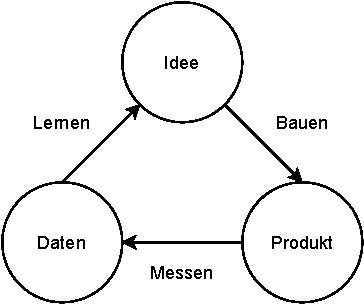
\includegraphics[width=0.5\columnwidth]{figures/lean-startup.pdf}
\caption{\label{fig:lean-startup}Iterationszyklus nach Lean Startup}
\end{figure}

Der Iterationszyklus ist in \autoref{fig:lean-startup} grafisch dargestellt\cite[vgl.][S. 75]{lean-startup}. Zunächst soll ein Produkt mit einer Idee starten. Diese Idee soll dann gebaut und anhand einer ausgewählten Metrik gemessen werden. Die Daten werden dann verwendet, um weitere Ideen zu generieren oder falsche Annahmen zu verwerfen. In dieser Arbeit wurden bereits mehrere Iterationszyklen durchlaufen, welche im Folgenden vorgestellt werden. \\

Zunächst ist die Idee entstanden, ein neues Rollenspiel in Anlehnung an Digimon World zu gestalten. Diese Idee wurde anhand von Interviews näher untersucht. Die daraus gewonnen Daten wurden analysiert und es sind neue Hypothesen aufgestellt worden. Dadurch ist die erste Iteration beendet worden. Die zweite Iteration startete mit den neu gewonnen Hypothesen. Eine Umfrage ist erstellt worden, welche erneut Daten generiert. In diesem Zyklus wurden Hypothesen belegt, aber einige auch widerlegt. Die quantitativen und qualitativen Daten wurden mit R untersucht und neue Erkenntnisse wurden geschlossen. Diese sind im dritten Iterationszyklus als Wireframes umgesetzt, welche mit unterschiedlichen Personen besprochen wurden. Während dieser Phase sind weitere Iterationszyklen im Bauen-Messen-Lernen-Zyklus entstanden, welche hier allerdings nicht näher erläutert werden. Im letzten Schritt wurden die gesammelten Daten zusammengetragen, um ein \ac{MVP} in der Godot Engine zu implementieren. Diese Daten müssen allerdings mit einer entsprechenden Metrik gemessen werden. \\

Für die Messung wird die Methode der schnellen iterativen Tests und Auswertungen(\ac{RITE}) verwendet\cite{rite-method}.
Die \ac{RITE}-Methode beschreibt ein Vorgehen, bei dem Testpersonen das Produkt testen und Probleme notiert werden. Diese werden in Form von Problemgruppen kategorisiert, welche sofort gelöst werden können, nach einiger Zeit gelöst werden können oder mehr Daten benötigt werden. In dieser Arbeit werden nur Probleme der ersten Kategorie abgehandelt. Alle weiteren Probleme werden nach der Arbeit bearbeitet. Getestet wird das \ac{MVP} von allen am Interview teilgenommenen Personen und dabei werden Probleme notiert. Diese Probleme sind im Repository als Issues in einer Kanban-Tafel aufgelistet.\\ 

\begin{figure}[H]
\centering
\begin{tikzpicture}
\begin{axis}[
    axis lines=middle,
    xmin=0, xmax=3,
    ymin=0, ymax=5,
    xtick={0, 1, 2, 3},
    ytick={1, 2, 3, 4, 5},
    x label style={at={(axis description cs:0.5,-0.1)},anchor=north},
    y label style={at={(axis description cs:-0.1,.5)},rotate=90,anchor=south},
    xlabel={Versuchsnummer},
    ylabel={Neu entdeckte Fehler},
    hide obscured x ticks=false,
    enlarge x limits={abs=10pt,upper},
    enlarge y limits={abs=10pt,upper},
]
\addplot [only marks, mark=o, mark options={blue,scale=2}] table {
1 5
2 4
3 2
};
\end{axis}
\end{tikzpicture}
\caption{\label{fig:rite-testing}Entdeckte Fehler im Testing}
\end{figure}

Nach jeder Testphase werden die Probleme zunächst gelöst, bevor die nächste Person die Testphase durchläuft. Auf diese Art und Weise können Lösungen bereits in der nächsten Testphase validiert werden und fallen nicht mehrfach auf. Alle, bis auf einen, Fehler in \autoref{fig:rite-testing} sind als Fehler der Stufe eins kategorisiert. Die Ausnahme bildet hierbei ein Fehler, welcher im ersten Versuch aufgefallen ist. Dieser konnte bis zum Versuch Nummer zwei nicht behoben werden und ist deswegen als Stufe zwei Fehler kategorisiert worden. Alle weiteren Fehler sind behoben worden. Es ist deutlich erkennbar, dass die erkannten Fehler für jeden weiteren Versuch abnehmen. Während jeder Testphase entstanden weitere Gespräche mit den Versuchspersonen und es wurde die Frage gestellt, ob die fertige Implementierung die Probleme der einzelnen Teilnehmenden lösen kann. Diese Frage wurde von allen teilnehmenden Personen bejaht.

\newpage
\section{Fazit und Ausblick}\label{sec:conclusion}
Das Ziel dieser Arbeit war es, herauszufinden, welche Probleme das Spiel Digimon World aufweist und wie diese behoben werden können. Um dieses Ziel zu erreichen, wurden zunächst Interviews durchgeführt, welche neue Erkenntnisse geliefert haben. Diese wurden in Form von Hypothesen in einer Online-Umfrage validiert. Die daraus resultierenden quantitativen Daten wurden dann verwendet, um Probleme zu ermitteln. Mithilfe von Methoden der nutzungsorientierten Gestaltung sind diese Probleme schließlich gelöst worden.\\

Die in dieser Arbeit entwickelte Anwendung soll als Machbarkeitsstudie angesehen werden. Das liegt daran, dass der Prototyp kein fertiges Produkt ist. Allerdings kann durch diese Anwendung gezeigt werden, dass die Entwicklung einige Fehler vermeidet, welche in Digimon World kritisiert wurden. 
Durch iteratives Weiterentwickeln kann die Anwendung zukünftig nutzungsoriert weiter optimiert werden.\\

Die Assets, welche in Zukunft noch in das Projekt eingebunden werden, könnten helfen, die Qualität des Spiels optisch zu verbessern. Dabei ist bereits bedacht, dass dies auch unbekannte Probleme mit sich bringen kann, welche infolgedessen untersucht werden müssen. Ein Beispiel hierfür wären verschiedene Varianten der Farbenfehlsichtigkeit. Ebenfalls müssen weitere Tests und Optimierungen vorgenommen werden, um das Produkt möglichst inklusiv zu gestalten. Der Charaktereditor löst zwar das Problem, dass das Geschlecht der spielenden Person einbezogen wird, allerdings wird die Hautfarbe aktuell noch vernachlässigt. Dieses und weitere Probleme können durch zusätzliche Interviews und Umfragen erforscht werden.\\

Abschließend lässt sich sagen, dass bis zur Veröffentlichung des Produkts weitere Iterationen nötig sind. Allerdings lässt sich die Frage, ob Inhalte des Spiels Digimon World verbessert werden können, positiv beantworten. Die dargestellten Ergebnisse rechtfertigen die Aussage, dass das neu entwickelte Videospiel Probleme in Digimon World löst. Ebenfalls kann davon ausgegangen werden, dass das Spiel künftig für eine größere Nutzergruppe zugänglich wird.

\newpage
\printbibliography

\appendix
\section{Anhang}
Im Anhang dieser Arbeit befindet sich der Interviewleitfaden, die entwickelten Personas, eine Übersicht über die 17 Hypothesen und weitere Streudiagramme.\\

Auf der beiliegenden DVD befindet sich die Arbeit und die Transkripte in Form einer PDF hinterlegt.
Ebenfalls sind dort die Handbücher für das Spiel Digimon World in japanischer, amerikanischer und deutscher Fassung als PDF.
Diesen Handbüchern ist der Fragebogen des Spiels, welcher in der amerikanischen Version beigelegt wurde, beigefügt.\\

Die verwendeten Daten für die Umfrage und die R-Skripte befinden sich ebenfalls auf der DVD.
Ebenso befindet sich der Code für das entwickelte Videospiel und eine ausführbare EXE auf der DVD.
Zusätzlich sind die konkreten Daten für die Auswertung in \autoref{table:game-engine-percent} als \ac{CSV} dem Anhang beigefügt.  \\

Die Transkripte, die Umfrage und der R-Code, sowie die Bachelorarbeit und das entwickelte Spiel sind auf GitHub zu finden\cite{github-transcripts}\cite{github-survey}\cite{github-bachelor-thesis}\cite{github-evo-world}.

\section{Interviewleitfaden}
Die nachfolgende \autoref{table:interview-guideline} stellt den Leitfaden dar, welcher in den Interviews verwendet wurde.
\begin{table}[h]
	\begin{center}
		\begin{tabularx}{\textwidth}{l|l|X}
			\textbf{Phase} & \textbf{Zweck} & \textbf{Fragen} \\
			\hline
			Einleitung & Erfassung personen- & Wie alt bist du? \\
            & bezogener Daten & Welchem Geschlecht fühlst du dich zugehörig? \\
            & & Fühlst du dich vorbereitet? 
            \newline \\
			Warm-Up    & Motivation & Welche anderen Spiele hast du in letzter Zeit in der Freizeit gespielt? \\
			& & Spielst du lieber mit Maus und Tastatur oder mit einem Controller? \\
			& & Nutzt du lieber eine Konsole oder einen Computer zum spielen?
			\newline \\
			Beobachtung & Emotionen & Welche Emotion wird gerade verspürt? \\
			& & Besteht eine Bindung zum digitalen Partner? \\
			& & Ist das Spiel immersiv? \newline \\
			& Aktionen & Woher weißt du \_\_\_? \\
			& & Wie findest du \_\_\_? \\
			& & Ist die aktuelle Aufgabe verständlich? \\
			& & Was ist dein aktueller Plan?
			\newline \\
			Abschluss & Rückblick und Fazit & Was wurde als gut empfunden? \\
			& & Was wurde als schlecht empfunden? \\
			& & Was ist die Meinung zum Kampfsystem? \\
			& & Wo hatte das Kampfsystem Stärken? \\
			& & Wo hatte das Kampfsystem Schwächen?
		\end{tabularx}
	\caption{Interviewleitfaden}
	\label{table:interview-guideline}
	\end{center}
\end{table}

\section{Personas}
Die nachfolgenden Personas beschreiben zwei fiktive Person, welche im Rahmen der Arbeit entstanden sind.

\begin{figure}[H]
  \centering
  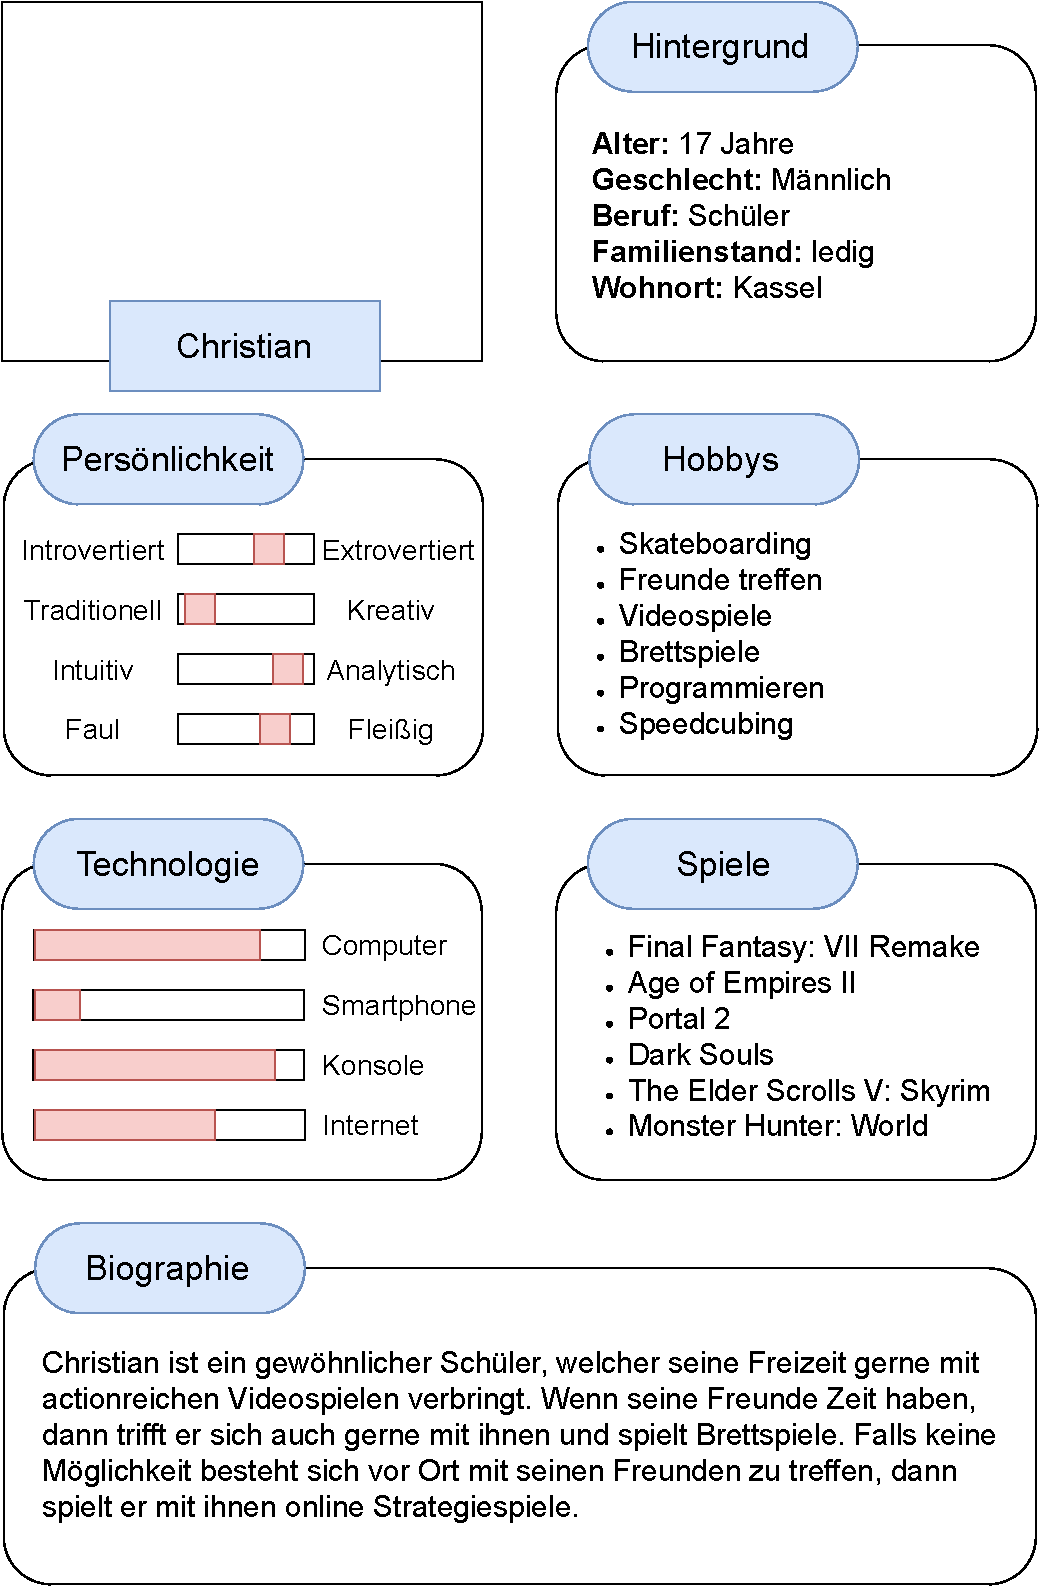
\includegraphics[width=0.83\columnwidth]{figures/Persona1.pdf}
  \caption{\label{fig:Persona1} Persona Christian}
\end{figure}


\begin{figure}[H]
  \centering
  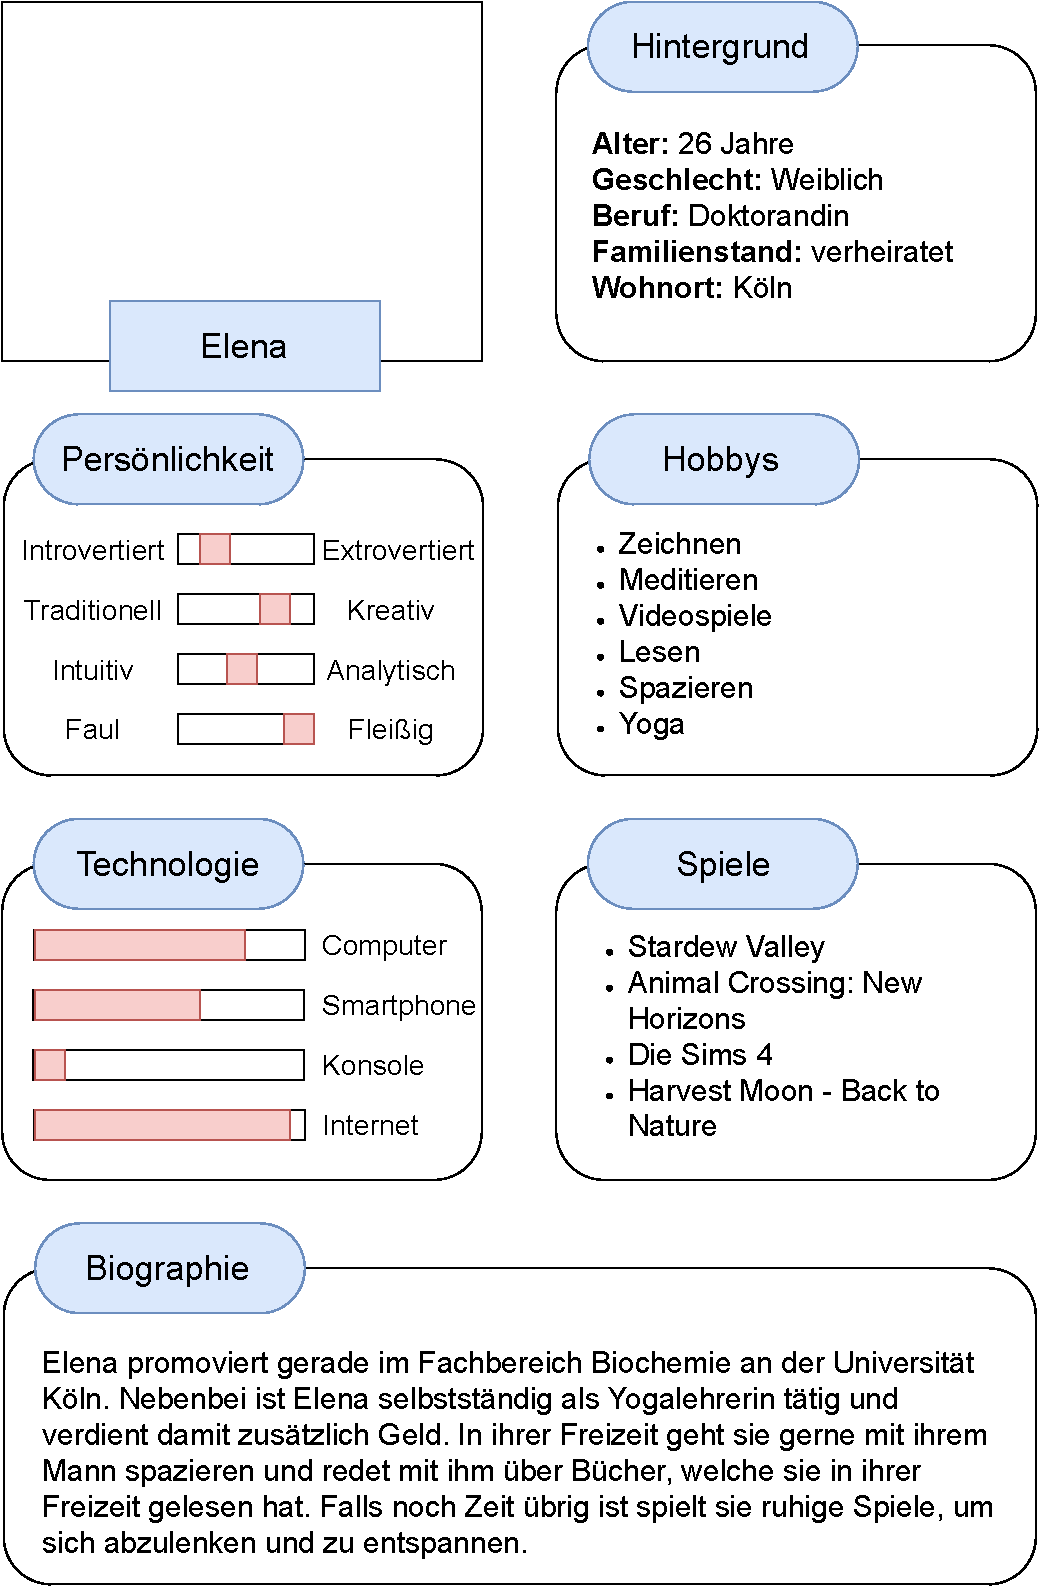
\includegraphics[width=0.83\columnwidth]{figures/Persona2.pdf}
  \caption{\label{fig:Persona2} Persona Elena}
\end{figure}

\section{Hypothesen im Überblick}
Die folgende \autoref{table:hypothesis-overview} zeigt alle in der Arbeit aufgestellten Hypothesen.
\begin{center}
   \begin{table}[!ht]
      \begin{tabular}{ c | l}
         Kennzeichen & Hypothese                                                                       \\
         \hline
         H1          & Eine neue Aufgabenliste soll helfen, die aktuellen Ziele des Spiels zu          \\
                     & identifizieren.                                                                 \\
         H2          & Items benötigen konkrete Werte, die angeben, wie sehr sich etwas nach           \\
                     & der Anwendung ändert. Zum Beispiel sollte \glqq Sättigt Digimon etwas\grqq{} in \\
                     & \glqq Sättigt Digimon etwas (+20 Nahrungspunkte)\grqq{} geändert werden.        \\
         H3          & Das Spiel benötigt zusätzliche Fortschrittsbalken für Essen oder Toilet-        \\
                     & tenbedarf.                                                                      \\
         H4          & Der Fortschrittsbalken für Glück und Disziplin sollte jeweils nicht in zwei     \\
                     & separate Fortschrittsbalken aufgeteilt werden.                                  \\
         H5          & Gesundheits- und Manapunkte sollten permanent auf dem HUD angezeigt             \\
                     & werden.                                                                         \\
         H6          & Gegenstände, die beim Verlust eines Herzens verloren gehen, sollten der         \\
                     & spielenden Person angezeigt werden.                                             \\
         H7          & Es sollte einen Indikator geben, der anzeigt, wie viel Zeit nach dem Trai-      \\
                     & ning oder anderen Aktivitäten vergeht, die eine bestimmte Zeit in An-           \\
                     & spruch nehmen.                                                                  \\
         H8          & Knöpfe, die zur Interaktion gedrückt werden können, sollten auf dem HUD         \\
                     & angezeigt werden.                                                               \\
         H9          & Die Uhr sollte einen Zeiger anstelle eines Punktes haben, der die aktuelle      \\
                     & Stunde anzeigt.                                                                 \\
         H10         & Tadeln sollte komplett aus dem Spiel entfernt werden.                           \\
         H11         & Es soll eine Minimap implementiert werden, die beim Navigieren durch            \\
                     & die Spielwelt hilft.                                                            \\
         H12         & Die Minimap sollte zusätzliche Informationen anzeigen. Zum Beispiel wo          \\
                     & NPCs, Essen oder die nächste Toilette ist.                                      \\
         H13         & Die spielende Person sollte in der Lage sein, ein Geschlecht auszuwählen.       \\
         H14         & Es sollte möglich sein, dem Charakter ein neues Aussehen zu geben.              \\
         H15         & Es sollte mehr Interaktionen während des Kampfes geben.                         \\
         H16         & Das Kampfsystem könnte rhythmusbasiert sein.                                    \\
         H17         & Anstelle eines Handbuchs sollte es ein Tutorial im Spiel geben.
      \end{tabular}
      \caption{Hypothesen im Überblick}
      \label{table:hypothesis-overview}
   \end{table}
\end{center}
\section{Streudiagramme}\label{sec:scatterplots}
Die nachfolgende \autoref{table:correlations-overview} zeigt die jeweiligen Korrelationen zwischen Hypothesen mit einem Korrelationskoeffizienten ohne Anwendung der Funktion \texttt{jitter}. Aufgrund dessen, dass der p-Wert unter dem festgelegten Signifikanzniveau $\alpha$ von $0,05$ liegt, sind die vorliegenden Korrelationen alle statistisch signifikant. 

\begin{table}[ht]
\centering
\begin{tabular}{ c | c | c | c}
  Relation & Spearmans $\rho$ & p-Wert & signifikant?\\
  \hline
  \hline
  H1 - H11 & $0,52$ & $1,1e-06$ & \cmark \\
  H1 - H12 & $0,54$ & $2,4e-07$ & \cmark \\
  H2 - H3 & $0,55$ & $1,5e-07$ & \cmark \\
  H11 - H12 & $0,76$ & $4,2e-16$ & \cmark \\
  H13 - H14 & $0,72$ & $9,5e-14$ & \cmark
\end{tabular}
\caption{Korrelationen zwischen Hypothesen im Überblick}
\label{table:correlations-overview}
\end{table}

Alle nachfolgenden Abbildungen zeigen Streudiagramme nach Anwendung der Funktion \texttt{jitter}. Diese wurde verwendet, um Werte voneinander unterscheiden zu können. Es sei angemerkt, dass dies R- und p-Werte verfälscht und die korrekten Werte in \autoref{table:correlations-overview} zu sehen sind.

\begin{figure}[H]
\centering
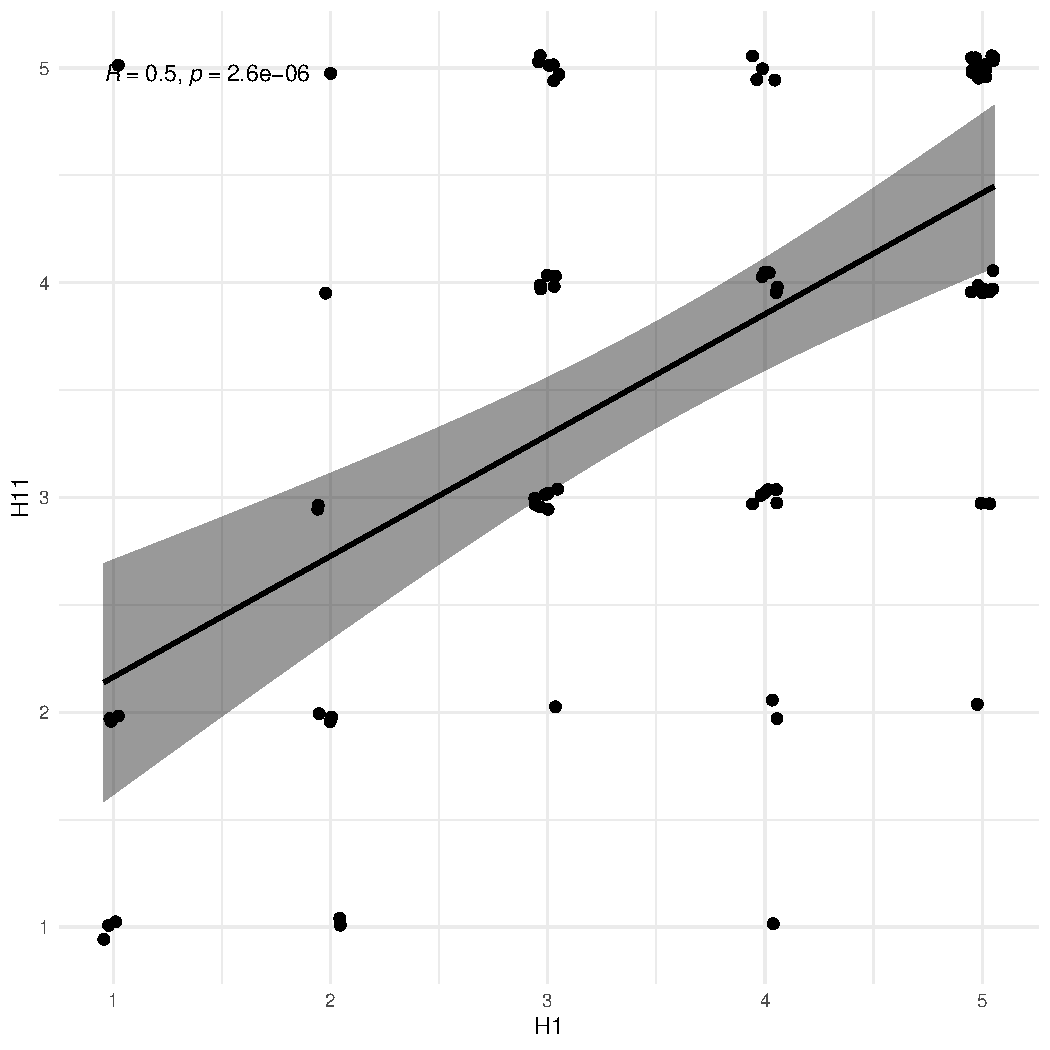
\includegraphics[width=0.65\columnwidth]{figures/plots/h1_h11.pdf}
\caption{\label{fig:h1-h11} Verwackeltes Streudiagramm - Korrelation zwischen H1 und H11}
\end{figure}

\begin{figure}[H]
\centering
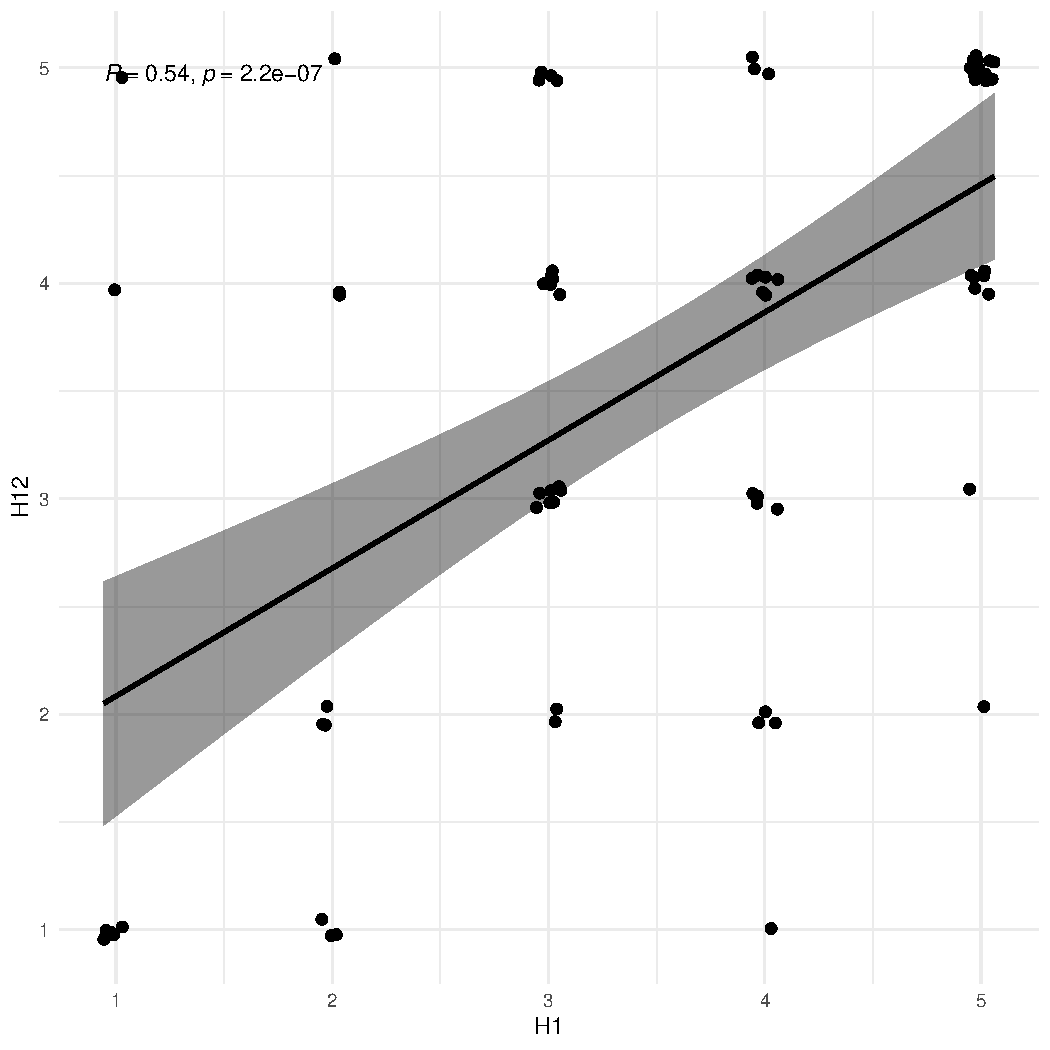
\includegraphics[width=0.65\columnwidth]{figures/plots/h1_h12.pdf}
\caption{\label{fig:h1-h12} Verwackeltes Streudiagramm - Korrelation zwischen H1 und H12}
\end{figure}

\begin{figure}[H]
\centering
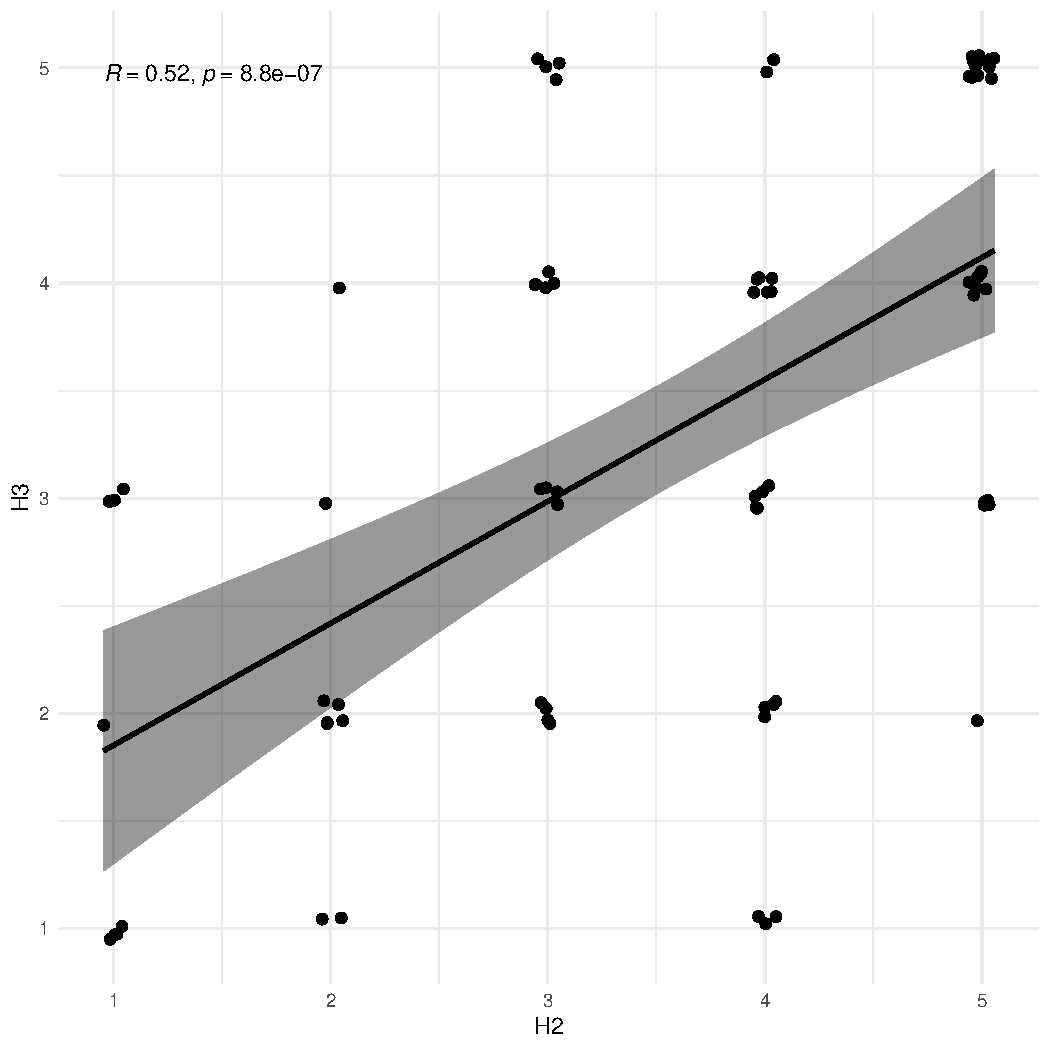
\includegraphics[width=0.65\columnwidth]{figures/plots/h2_h3.pdf}
\caption{\label{fig:h2-h3} Verwackeltes Streudiagramm - Korrelation zwischen H2 und H3}
\end{figure}


\begin{figure}[H]
\centering
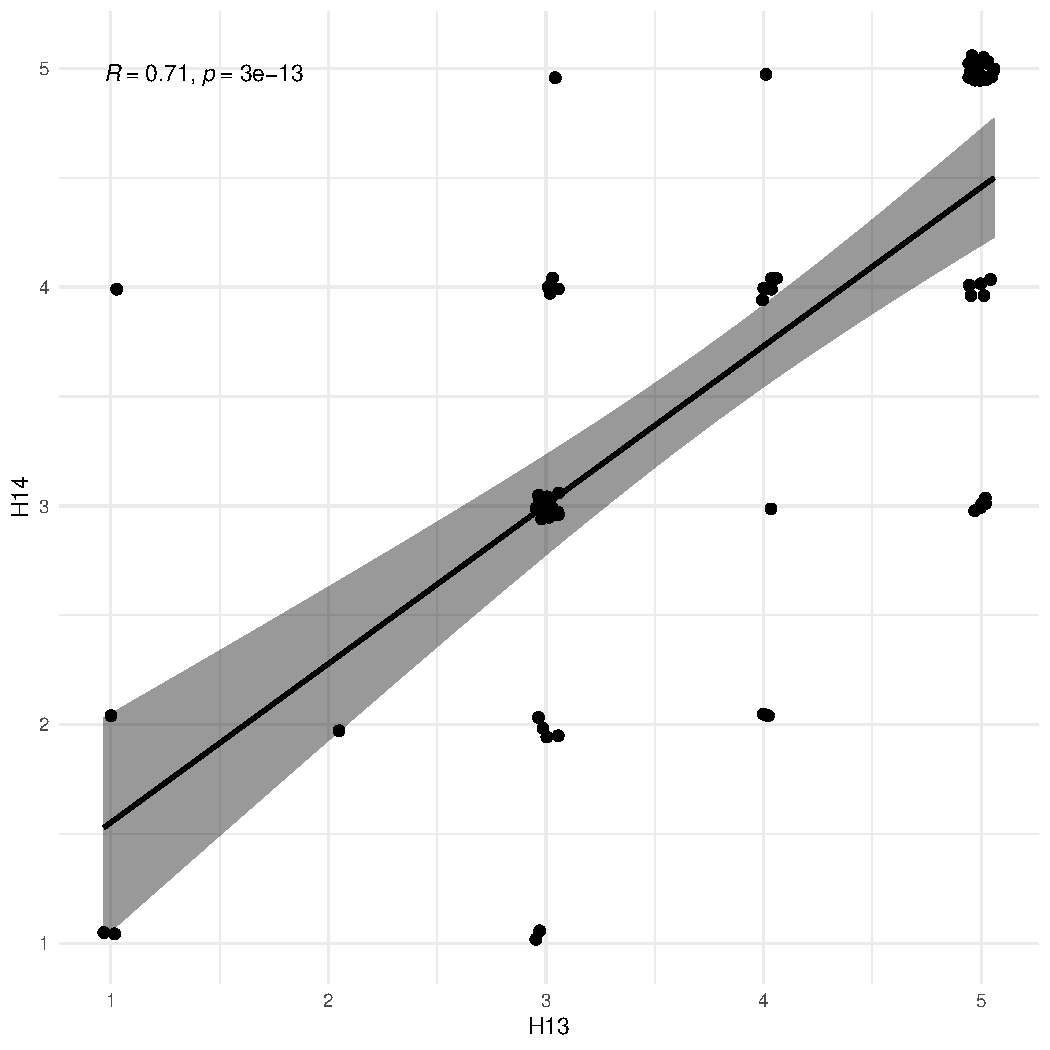
\includegraphics[width=0.65\columnwidth]{figures/plots/h13_h14.pdf}
\caption{\label{fig:h13-h14} Verwackeltes Streudiagramm - Korrelation zwischen H13 und H14}
\end{figure}


\end{document}
